\documentclass[
  a4paper,
  12pt,
  headsepline,
  numbers=noenddot,
  captions=oneline,
  captions=tableheading,
  BCOR12mm,
  headinclude,
  chapterprefix,
  appendixprefix,
  index=totoc,
  bibliography=totoc
]{scrbook}

\usepackage{dissertation}
\usepackage{scrhack}
\usepackage{color}

%load any additional packages
\usepackage{amssymb}

% for a whitespace behind newcommand items
\usepackage{xspace}
\usepackage{xcolor}

%For equations
\usepackage{amsmath,amssymb}
\usepackage{bm}
\newcommand{\argmax}{\operatornamewithlimits{argmax}}
\newcommand{\argmin}{\operatornamewithlimits{argmin}}
\newcommand{\ci}{\mathrel{\text{\scalebox{1}{$\perp\mkern-10mu\perp$}}}}

% For algorithms
\usepackage{algorithm}
\usepackage{algorithmic}

% For figures
\usepackage{subfigure}
\usepackage{tikz}
\usetikzlibrary{bayesnet,matrix,calc}
\usepackage{graphicx}
\newcommand{\mycaption}[2]{\caption{\textbf{#1.}\xspace#2}}
\usepackage{pbox}
\usepackage{wrapfig}

%For tables
\usepackage{booktabs}
\usepackage{array}
\usepackage{multirow}
\usepackage{multicol}
\usepackage{longtable}

%For bibliography
\usepackage{natbib}
\usepackage{bibentry}

\setcitestyle{square,numbers,comma}

%For URLs
\usepackage{hyperref}

%
% P L E A S E
%
% Enter your name, the title and some keywords for this document here:
%
\degree{}
\name{Varun Jampani}
\thesis{Learning Inference Models for Computer Vision}
\keywordlist{Computer Vision, Machine Learning, Inference, Generative Models,
Discriminative Models, Deep Learning}
\hometown{Tenali, Indien}

\dean{Prof.~Dr.~Wolfgang Rosenstiel}

\reviewerone{Prof.~Dr.~Hendrik P.~A. Lensch}
\reviewertwo{Prof.~Dr.~Peter V. Gehler}
\reviewerthree{Dr.~Iasonas Kokkinos}



% \doublespacing

% Type the hyphonation of important words here:
\selectlanguage{english}
\hyphenation{
Hello
Gen-ome
sub-stan-ce
me-ta-bo-li-sm
con-cen-tra-ti-ons
}

%%%%%%%%%%%%%%%%%%%%%%%%
\hypersetup{
              %bookmarks={true},
              bookmarksopen={true},
              bookmarksopenlevel={0},
              bookmarksnumbered={true},
              breaklinks={true},
              colorlinks={false},
              pdfpagemode={UseOutlines},
              pdftitle={\thethesis},
              pdfauthor={\thename},
              pdfsubject={Dissertation},
              pdfkeywords={\thekeywordlist},
              pdfview={FitV},
              %pdftex,
              pdffitwindow={true},
              pdfstartview={FitV},
              pdfnewwindow={false},
              pdfdisplaydoctitle={true},
              pdfhighlight={/P},
              plainpages={false},
              unicode={true},
              urlcolor={blue}
}
\extratitle{\begin{center}\normalfont\sffamily\thethesis\end{center}}
\title{\thethesis}
\author{\Large Dissertation\\
\normalsize der Mathematisch-Naturwissenschaftlichen Fakult\"at\\
\normalsize der Eberhard Karls Universit\"at T\"ubingen\\
\normalsize zur Erlangung des Grades eines\\
\normalsize Doktors der Naturwissenschaften\\
\normalsize (Dr.~rer.~nat.)}
\date{\ \\[2ex]\normalsize  vorgelegt von\\
%\Large \thedegree~\thename\\
\Large \thename\\
\normalsize aus \thehometown}
\publishers{\normalsize T\"ubingen\\\normalsize 2016}
\lowertitleback{
Gedruckt mit Genehmigung der Mathematisch-Naturwissenschaftlichen Fakult\"at der
Eberhard Karls Universit\"at T\"ubingen. \\
\\
\begin{tabular}{lp{.55\textwidth}}
Tag der m\"undlichen Qualifikation:& 02.05.2017\\
Dekan:                             & \thedean\\
1.~Berichterstatter:               & \thereviewerone\\
2.~Berichterstatter:               & \thereviewertwo\\
3.~Berichterstatter:               & \thereviewerthree\\
\end{tabular}}
\dedication{\normalsize To my grandfather \emph{K. Anjaneyulu}} % Change or remove this!

% This command is useful to edit and compile only one or a selection of some
% files instead of the whole document. This is very useful and facilitates
% editing these large documents.
% \includeonly{tex/Fil1 tex/File2...}

% \makeatletter\@addtoreset{chapter}{part}\makeatother%

\DeclareOldFontCommand{\bf}{\normalfont\bfseries}{\mathbf}

\begin{document}
\frontmatter
\selectlanguage{ngerman}
\maketitle
\selectlanguage{english}

%
% Caution: Abstract, Kurzfassung, and Acknowledgements are chapter* (in this
%          way they don't occur in the table of contents)! However, this
%          means, you have to set the headline manually (see the example files)
%
  In this paper, we explore the connection between secret key agreement and secure omniscience within the setting of the multiterminal source model with a wiretapper who has side information. While the secret key agreement problem considers the generation of a maximum-rate secret key through public discussion, the secure omniscience problem is concerned with communication protocols for omniscience that minimize the rate of information leakage to the wiretapper. The starting point of our work is a lower bound on the minimum leakage rate for omniscience, $\rl$, in terms of the wiretap secret key capacity, $\wskc$. Our interest is in identifying broad classes of sources for which this lower bound is met with equality, in which case we say that there is a duality between secure omniscience and secret key agreement. We show that this duality holds in the case of certain finite linear source (FLS) models, such as two-terminal FLS models and pairwise independent network models on trees with a linear wiretapper. Duality also holds for any FLS model in which $\wskc$ is achieved by a perfect linear secret key agreement scheme. We conjecture that the duality in fact holds unconditionally for any FLS model. On the negative side, we give an example of a (non-FLS) source model for which duality does not hold if we limit ourselves to communication-for-omniscience protocols with at most two (interactive) communications.  We also address the secure function computation problem and explore the connection between the minimum leakage rate for computing a function and the wiretap secret key capacity.
  
%   Finally, we demonstrate the usefulness of our lower bound on $\rl$ by using it to derive equivalent conditions for the positivity of $\wskc$ in the multiterminal model. This extends a recent result of Gohari, G\"{u}nl\"{u} and Kramer (2020) obtained for the two-user setting.
  
   
%   In this paper, we study the problem of secret key generation through an omniscience achieving communication that minimizes the 
%   leakage rate to a wiretapper who has side information in the setting of multiterminal source model.  We explore this problem by deriving a lower bound on the wiretap secret key capacity $\wskc$ in terms of the minimum leakage rate for omniscience, $\rl$. 
%   %The former quantity is defined to be the maximum secret key rate achievable, and the latter one is defined as the minimum possible leakage rate about the source through an omniscience scheme to a wiretapper. 
%   The main focus of our work is the characterization of the sources for which the lower bound holds with equality \textemdash it is referred to as a duality between secure omniscience and wiretap secret key agreement. For general source models, we show that duality need not hold if we limit to the communication protocols with at most two (interactive) communications. In the case when there is no restriction on the number of communications, whether the duality holds or not is still unknown. However, we resolve this question affirmatively for two-user finite linear sources (FLS) and pairwise independent networks (PIN) defined on trees, a subclass of FLS. Moreover, for these sources, we give a single-letter expression for $\wskc$. Furthermore, in the direction of proving the conjecture that duality holds for all FLS, we show that if $\wskc$ is achieved by a \emph{perfect} secret key agreement scheme for FLS then the duality must hold. All these results mount up the evidence in favor of the conjecture on FLS. Moreover, we demonstrate the usefulness of our lower bound on $\wskc$ in terms of $\rl$ by deriving some equivalent conditions on the positivity of secret key capacity for multiterminal source model. Our result indeed extends the work of Gohari, G\"{u}nl\"{u} and Kramer in two-user case.        % In case this work is to be written in German,
                              % no English abstract is required.
\selectlanguage{ngerman}
\chapter{Zusammenfassung}

Maschinelles Sehen kann als die F\"ahigkeit verstanden werden Bilddaten zu interpretieren. Durchbr\"uche in diesem Feld gehen oft einher mit Fortschritten in Inferenztechniken, da die Komplexit\"at der Inferenz die Komplexit\"at der verwendeten Modelle bestimmt. Diese Arbeit beschreibt lernbasierte Inferenzmechanismen und zeigt Anwendungen im maschinellen Sehen auf, wobei auf Techniken f\"ur Inferenz in sowohl generativen als auch diskriminativen Modellen eingegangen wird.


Obwohl naheliegend und intuitiv verst\"andlich, sind generative Modelle im maschinellen Sehen h\"aufig nur eingeschr\"ankt nutzbar, da die Berechnung der A-Posteriori-Wahrscheinlichkeiten oft zu komplex oder zu langsam ist, um praktikabel zu sein. Wir beschreiben Techniken zur Verbesserung der Inferenz in zwei weit verbreiteten Inferenzverfahren: `Markov Chain Monte Carlo Sampling' (MCMC) und `Message-Passing'. Die vorgeschlagene Verbesserung besteht darin, mehrere diskriminative Modelle zu lernen, die die Grundlage f\"ur Bayes'sche Inferenz \"uber einem generativen Modell bilden. Wir demonstrieren anhand einer Reihe von generativen Modellen, dass die beschriebenen Techniken den Inferenzprozess beschleunigen und/oder zu besseren L\"osungen konvergieren.


Eine der gr\"o{\ss}ten Schwierigkeiten bei der Verwendung von diskriminativen Modellen ist die systematische Ber\"ucksichtigung von Vorkenntnissen. Zur Verbesserung der Inferenz in diskriminativen Modellen schlagen wir Techniken vor die das ursprüngliche Modell selbst verändern, da Inferenz in diesen die schlichte Auswertung des Modells ist. Wir konzentrieren uns auf `Convolutional Neural Networks' (CNN) und schlagen eine Generalisierung der Faltungsoperation vor, die den Kern jeder CNN-Architektur bildet. Dazu verallgemeinern wir bilaterale Filter und pr\"asentieren eine neue Netzarchitektur mit trainierbaren bilateralen Filtern, die wir `Bilaterale Neuronale Netze' nennen. Wir zeigen, wie die bilateralen Filtermodule verwendet werden können, um existierende Netzwerkarchitekturen für Bildsegmentierung zu verbessern und entwickeln ein auf Bilateralen Netzen basierendes Modell zur zeitlichen Integration von Information für Videoanalyse. Experimente mit einer breiten Palette von Anwendungen und Datens\"atzen zeigen das Potenzial der vorgeschlagenen bilateralen Netzwerke.


Zusammenfassend schlagen wir Lernmethoden f\"ur bessere Inferenz in einer Reihe von Modellen des maschinellen Sehens vor, von inversen Renderern bis zu trainierbaren neuronalen Netzwerken. Unsere Inferenz-Techniken helfen bei der Berechnung der A-Posteriori-Wahrscheinlichkeiten in generativen Modellen und erm\"oglichen so neue Ans\"atze des modellbasierten machinellen Lernens im Bereich des maschinellen Sehens. In diskriminativen Modellen wie CNNs helfen die vorgeschlagenen verallgemeinerten Filter beim Entwurf neuer Netzarchitekturen, die sowohl hochdimensionale Daten verarbeiten k\"onnen als auch Vorkenntnisse in die Inferenz einbeziehen.
     % In any case you have to write a German abstract.
\selectlanguage{english}
\documentclass{article}

\begin{document}

\section{Acknowledgements}

The author would like to thank B. J. Hiley, M. Hajtanian, and D. Nellist for their insightful conversations and support.

\end{document} % If you want to write your acknowledgements in
                              % German please move the selectlanguage command

\tableofcontents

\chapter{Symbols and Notation}
\label{chap:symbols}

\newcommand{\obs}{\mathbf{x}}
\newcommand{\target}{\mathbf{y}}
\newcommand{\targetProp}{\bar{\mathbf{y}}}
\newcommand{\params}{\mathbf{\theta}}
\newcommand{\f}{\mathbf{f}}
\newcommand{\func}{\mathcal{F}}

\newcommand{\eg}{\textit{e.g.}\@\xspace}
\newcommand{\ie}{\textit{i.e.}\@\xspace}
\newcommand{\ala}{\textit{\'{a}~la}\@\xspace}
\newcommand{\etal}{\textit{et~al.}\@\xspace}

Unless otherwise mentioned, we use the following notation and symbols in this
thesis. Here, we only list those symbols which are used across multiple chapters.
Those symbols that are specific to particular sections or chapters are not
listed here.

\begin{longtable}[l]{p{50pt} p{300pt}}
\toprule
\textbf{Symbol}	& \textbf{Description} \\
\midrule
$\obs$	 	& Observation variables (in vectorized form)\\
$\target$	 	& Target variables (in vectorized form)\\
$\targetProp$	 	& Intermediate/Proposed target variables\\
$K_t,m_t,\cdots$	 	& Random variables at time step $t$\\
$\params$	 	& Set of all model parameters \\
$\alpha, \beta, \mu, \gamma$	 & Model or training parameters \\
$\f$	 	& Pixel or superpixel features such as $(x,y,r,g,b)$ \\
$P(\cdot|\cdot)$	&  Probability distribution or density \\
$\mathcal{N}(\cdot|\cdot)$	& Gaussian distribution \\
$\psi_u$ & Unary potential at each pixel/superpixel \\
$\psi_p$ & Pairwise potential between two pixels/superpixels \\
$L(\cdot), E(\cdot)$ & Loss/Objective/Energy function \\
$\func(\cdot)$ & Generic function relating input to output variables \\
$\Lambda$ & Diagonal matrix for scaling image features say $(x,y,r,g,b)$ \\
\bottomrule
\end{longtable}

\chapter{Acronyms}
\label{chap:abbrv}
\vspace{-0.5cm}
\begin{longtable}[l]{p{80pt} p{300pt}}
\toprule
\textbf{Acronym}	& \textbf{Full Form} \\
\midrule
AR & Acceptance Rate \\
BCL	 	& Bilateral Convolutional Layer\\
BI	 	& Bilateral Inception\\
BNN	 	& Bilateral Neural Network\\
BP & Belief Propagation \\
CMP & Consensus Message Passing \\
CNN	 	& Convolutional Neural Network\\
CPU & Central Processing Unit \\
CRF & Conditional Random Field \\
DDMCMC & Data Driven Markov Chain Monte Carlo\\
EP & Expectation Propagation \\
FC & Fully Connected \\
GPU & Graphics Processing Unit \\
IoU & Intersection over Union \\
INF-INDMH	 	& Informed Independent Metropolis Hastings\\
INF-MIXMH	 	& Informed Mixture Metropolis Hastings\\
INF-MH	 	& Informed Metropolis Hastings\\
KDE & Kernel Density Estimation \\
MAP & Maximum a Posteriori \\
MCMC 	& Markov Chain Monte Carlo\\
MF & Mean-Field \\
MH	 	& Metropolis Hastings\\
MHWG & Metropolis Hastings Within Gibbs \\
MP & Message Passing \\
PGM  & Probabilistic Graphical Model \\
PSNR & Peak Signal to Noise Ratio \\
PSRF & Potential Scale Reduction Factor \\
PT & Parallel Tempering \\
REG-MH & Regenerative Metropolis Hastings \\
RF & Random Forest \\
RMSE & Root Mean Square Error \\
VMP & Variational Message Passing \\
VPN & Video Propagation Network \\
\bottomrule
\end{longtable}


\mainmatter
% Content



\section{Introduction}
\label{sec:intro}

% background
Recent years have witnessed a rapid growth of longitudinal studies with binary and 
ordinal responses in several disciplines, including econometrics, and the health 
and social sciences. In such studies, of primary importance are the probability 
response curves, i.e., the probabilities of the response categories that evolve
dynamically over time.
%known as the probability response curves. Because of its potential to address 
%relevant scientific and practical questions, inference for these curves is of 
%primary importance. 
This article aims at developing a hierarchical framework, 
customized to longitudinal settings, that allows flexible inference for the probability 
response curves. In addition, the defining characteristic of longitudinal data is that 
repeated measurements on the same subject induce dependence. Hence, a further objective 
is to %accurately identify 
flexibly model lead-lag correlations among repeated measurements. 


% research objective, also mention that we focus on the case without covariates/with categorical covariates

%The defining characteristic of a longitudinal study is that subjects are measured repeatedly through time \citep{DiggleBook2002}. With longitudinal data, one can differentiate the changes over time within subjects (aging effects) from the changes between subjects at baseline (cohort effects). The objectives of analysis include assessing the fluctuation within a subject over time and identifying lead-lag correlations among repeated measurements. In certain applications where features associated with the measurements are also available, regressing longitudinal ordinal outcomes on these fixed covariates is also of interest.  In this article, we focus particularly on developing flexible modeling approach for estimate the probability response curves, which can be viewed as the regression relationship with time as the only covariates. Nonetheless, we discuss including other categorical covariates as a natural extension of the proposed method. 

%Nonetheless, the benefit comes at a price of modeling challenges. The major challenges arise from the two objectives of analyzing longitudinal data: capturing the fluctuation and dependency among the repeated measurements. Consequently, more sophisticated statistical methods are needed. Note that usually repeated measurements come along with features of the subjects, forming up regression problems.  

% parametric GMM modeling framework
%The development of statistical methods for longitudinal binary data stems from models for longitudinal continuous responses. Since the most natural way to view binary data is to postulate the existence of a latent continuous variable associated with each response, such models can be extended to deal with binary data through appropriate link function. A plethora of literature have covered the topic of longitudinal continuous data analysis \citep{HedekerGibbons2006,Verbeke2009,Fitzmaurice2011}, with the majority of them under the mixed effects modeling framework. Suppose we have repeated measurements on $n$ subjects, denoted as $\mathbf{Z}_i=(Z_{i1},\cdots,Z_{iT_i})^T$, $i=1,\cdots,n$. Typically the mixed effects model assumes $\mathbf{Z}_i\sim N(\mathbf{u},\mathbf{V}_i)$, where $\mathbf{u}$ denote the common fixed effect across subjects, and $\mathbf{V}_i$ is the random subject effect that depicts the influence of subjects on their repeated observations \citep{Diggle1988}. The crucial question for the mixed effects model is the choice of fixed and random effects' structure, which has various options \citep{Lindstrom1990,Shi1996,Zhang2001}. These models have been extended to deal with dichotomous data by adopting a link function (logit, probit, etc.), resulting in the generalized mixed models (GMM). For a comprehensive review about GMM, we refer to \citet{Hedeker2008}.
%These models have been extended to deal with dichotomous and ordinal data by adopting a link function (logit, probit, etc.), and a specific representation of response probabilities (proportional odds, adjacent-categories, continuation-ratio, etc.), resulting in the generalized mixed models (GMM). For a comprehensive review about GMM, we refer to \citet{Hedeker2008}. 

% nonparametric modeling approaches
%Seeking for more flexibility, one option is to assume the fixed or random effects of the latent variable have more sophisticated, nonparametric structure. Popular choices include modeling the fixed effect through smoothing techniques \citep{HeZhu2002,WuZhang2006}, applying a matrix stick-breaking process for a residual covariance structure \citep{Das2014}, capturing subject random effect by stochastic process \cite{ZhangLin1998}, putting a Dirichlet process (DP) prior \citep{LiLinMuller2010} or mixture of Pólya trees \citep{Ghosh2010} for random effect distributions, and using a combination of stochastic processes and DP mixture model for the subject random effect \citep{Quintana2016}. Admittedly, such models can be embedded in a hierarchical framework to deal with discrete responses. For instance, under the GMM framework which incorporate a DP mixture of normal prior as probability model for the latent variables,  \citet{Jara2007} and \citet{TangDuan2012} consider binary responses and \citet{Kunihama2019} handles mixed-scale data consisted by continuous and binary responses. Nonetheless, these approaches may not be applicable beyond dichotomous responses because of the computational burden. Concerning multivariate longitudinal ordinal responses, \citet{Tran2021} proposes to use a latent factor model within the GMM framework where the random effect is modeled by Ornstein-Uhlenbeck process. Albeit its good performance, the proposed model is restrictive in the sense that it depends on pre-specified covariance structure. In conclusion, these models are trading between flexibility and computational difficulty. Even though they achieved the balance for their specific purpose respectively, they are not the ideal option for the specific problem we considered. Besides, they examine the mean and covariance structure of the latent variable separately, which may neglect their dependence. 

% review transition modeling framework
%To evaluate the fixed and random effects jointly, one option is to follow the transition modeling framework \citep[see][chap.~10]{DiggleBook2002}. Under a transition model, the past value explicitly affect the present observation, inducing the aging effects. Therefore, the proposed models under this framework typically assume autoregressive transition dynamics between the distribution of responses at adjacent time.  \citet{DiLucca2013} develop a class of Bayesian nonparametric autoregression models. They model a sequence of continuous outcomes though a dependent DP with an additional normal kernel as a prior for the regression on lagged terms in an autoregression. It can be extended to handle binary and ordinal outcomes by treating the them as the discretized version of the continuous outcomes. In addition, motivated by a specific application in fisheries science, \citet{MariaJASA2018} propose a Bayesian nonparametric model for ordinal regression relationships that evolve in discrete time. Their proposed methodology is built on the well-studied DP mixture model for cross-sectional ordinal regression \citep{DeYoreoKottas2018} as the marginal at a specific time, while introduce temporal dependence in the weights and atoms of the DP constructive definition. Although autoregressive structure brings benefits such as interpretability, there is no natural way to treat missing data, hindering the application in unbalanced longitudinal studies.    

%Under the GMM framework, the mean and covariance structure of the latent variable are examined separately, which may neglect their dependence. To incorporate the possible dependence among them, one option is to follow the transition modeling framework \citep[see][chap.~10]{DiggleBook2002}. Under a transition model, the past value explicitly affect the present observation, inducing the aging effects. The proposed models under this framework typically assume autoregressive transition dynamics between the distribution of responses at adjacent time. Although autoregressive structure brings benefits such as interpretability, there is no natural way to treat missing data, hindering the application in unbalanced longitudinal studies.


The development of statistical methods for longitudinal binary and ordinal data stems from 
models for longitudinal continuous responses, postulating the generalized linear model framework. 
Analogous to the continuous case, a specific model is formulated under one of three broad
approaches pertaining to marginal models, conditional models, or subject-specific models. 
Marginal models provide alternative modeling options when likelihood-based approaches are 
difficult to implement.
%A marginal model captures the responses by their marginal distribution given the covariates. 
A conditional model describes the distribution of responses conditional on the covariates 
and also on part of the other components of the responses. In a subject-specific model, 
the effects of a subset of covariates are allowed to vary randomly from one individual 
to another. In the absence of predictor variables, functions of the observation time are 
usually used as covariates. We refer to \citet{Molenberghs2006} for a comprehensive review. 
In Section \ref{subsec:literaturereview}, we elaborate on the connection of our 
proposed modeling approach with existing methods.


%our approach
In this article, we introduce a novel viewpoint for longitudinal binary and ordinal data 
analysis. %which directs a path for new discoveries. 
We begin with the model construction for longitudinal binary responses. The critical insight 
that distinguishes our methodology from the majority of the existing literature is functional 
data analysis. We treat the subjects' measurements as stochastic process realizations at the 
corresponding time points. The benefits are twofold. First, the models can incorporate 
unbalanced data from longitudinal studies in a unified scheme; directly inferring the 
stochastic process provides a well-defined probabilistic model for the missing values. 
Secondly, we can exploit the power of Bayesian hierarchical modeling for continuous 
functional data \citep[e.g.,][]{Yang2016}. To that end, we adopt the Binomial distribution 
with the logit link that connects binary responses to continuous signals, which, subject to 
%a common level of 
additive measurement error, are then modeled as (conditionally) independent and 
identically distributed (i.i.d.) realizations from a Gaussian process (GP) with 
random mean and covariance function. We place an Inverse-Wishart process (IWP) prior 
on the covariance function, and conditional on it, use a GP prior for the mean function. 
Therefore, the two essential ingredients in longitudinal modeling, the trend and the 
covariance structure, are modeled simultaneously and nonparametrically. 


The hierarchical structure allows borrowing of strength across the subjects' trajectories. 
We apply a specific setting of hyperpriors for the GP and IWP priors, such that marginalizing 
over them, the latent continuous functions have a Student-t process (TP) prior. The 
TP enhances the flexibility of the GP \citep[e.g.,][]{Shah2014}. It retains attractive GP 
properties, such as analytic marginal and predictive distributions, and it yields 
predictive covariance that, unlike the GP, explicitly depends on the observed values. 
% what are the benefit?
For inferential purposes, we represent the joint posterior distribution in multivariate form 
through evaluating the functions on the pooled grid, resulting in the common 
normal-inverse-Wishart conditional conjugacy. In conjunction with the Pólya-Gamma data 
augmentation technique \citep{Polson2013}, we develop a relatively simple and effective posterior 
simulation algorithm, circumventing the need for specialized techniques or tuning of 
Metropolis-Hastings steps. 


To extend the model for ordinal responses, we utilize the continuation-ratio logits 
representation of the multinomial distribution. Such representation features an %interchangeable 
encoding of an ordinal response with $C$ categories as a sequence of $C-1$ binary 
indicators, in which the $j$-th indicator signifies whether the ordinal response belongs 
to the $j$-th category or to one of the higher categories. 
%As shown in Proposition \ref{prop:fitseparate}, 
We show that fitting a multinomial model for the ordinal responses is equivalent 
to fitting separately the aforementioned model on the binary indicators. 
%As a consequence, the model for longitudinal ordinal responses inherits the features of 
%the model for binary responses. Furthermore, 
Hence, we can conduct posterior simulation for each response category in a parallel fashion, 
leading to significant computational efficiency gains in model implementation.       


% about the missingness
In modern longitudinal studies, it is common that the complete vector of repeated measurements 
is not collected on all subjects. As a specific example, in ecological momentary assessment 
(EMA) studies, emotions and behaviors are repeatedly measured for a cohort of participants, 
through wearable electronic devices \citep{EMABook2018}. For instance, in the \textit{StudentLife} 
study \citep{StudentLife2014}, researchers monitored the students' mental status through 
pop-up questionnaires on their smartphones that prompted multiple times at pseudorandom 
intervals during the study period. Since the data collection process is based on the 
participants' conscious responding to prompted questions several times a day, non-response 
is inevitable. Missing values are typically considered to be a nuisance rather than a 
characteristic of EMA time series. Parametric and nonparametric Bayesian methods have been 
developed to handle longitudinal data with missingness; see \citet{Daniels2020} for a review. 
The common issue is that one has to bear the drawbacks of making either structured or 
unstructured assumptions to manage missingness. The unstructured approach leads to flexibility, 
yet it may result in difficulties due to a large number of parameters relative to the sample 
size. Besides, the majority of the existing literature on longitudinal studies with missingness 
focuses on the scenario with continuous responses, and the extension to discrete responses is not trivial. 


% summary of our contribution
Accordingly, our contributions can be summarized as follows: (i) we model the mean and 
covariance jointly and nonparametrically, avoiding potential biases caused by a pre-specified 
model structure; (ii) we unify the toolbox for balanced and unbalanced longitudinal studies; 
(iii) the model encourages borrowing of strength, preserving systematic patterns that are 
common across all subject responses; (iv) we develop a computationally efficient posterior 
simulation method by taking advantage of conditional conjugacy; (v) the model facilitates 
applications for ordinal responses with a moderate to large number of categories. 
% and parallel computing.    


% organization of the paper
The rest of the paper is organized as follows. 
%We start from emphasizing the pivotal model designs and benefits with longitudinal 
%binary responses in Section \ref{sec:binarymodel} and Section \ref{sec:realapp}, 
%as it lays the foundation for the extension to ordinal responses. In more detail, 
Section \ref{sec:binarymodel} develops the methodology for binary responses, including
model formulation, study of model properties, and the computational approach to 
inference and prediction.
%In Section \ref{sec:simstudy}, we assess the model by applying it to carefully designed 
%simulation scenarios that reflect our main contributions. 
Section \ref{sec:realapp} illustrates the modeling approach through an EMA study that 
focuses on analyzing students' mental health through binary outcomes. The modeling extension 
for longitudinal ordinal responses is presented in Section \ref{sec:polyordinalmodel}, 
including an illustration involving an ordinal outcome from the same EMA study. Finally, 
Section \ref{sec:summary} concludes with a summary.



 
\section{Incremental scaling and squaring}
\label{sec:scaling_and_squaring}

Since the set of conformally partitioned block triangular matrices
forms an algebra, and $\exp(G_n)$ is a polynomial in $G_n$, the matrix
$\exp(G_n)$ has the same block upper triangular structure as $G_n$, that is,
\begin{equation*}
    \exp(G_n) =
    \begin{bmatrix}
        \exp(G_{0,0}) & \ast          & \cdots & \ast \\
                      & \exp(G_{1,1}) & \ddots & \vdots \\
                      &               & \ddots & \ast  \\
                      &               &        & \exp(G_{n,n}) \\
    \end{bmatrix}
    \in \R^{d_n \times d_n}.
\end{equation*}
As outlined in the introduction, we aim at computing $\exp(G_n)$ block
column by block column, from left to right.  Our algorithm is based on
the scaling and squaring methodology, which we briefly summarize
next.

\subsection{Summary of the scaling and squaring method}
\label{sec:scaling_squaring}

The scaling and squaring method uses a rational function to
approximate the exponential function, and typically involves three
steps. Denote by $r_{k,m}(z) = \frac{p_{k,m}(z)}{q_{k,m}(z)}$ the
$(k,m)$-Pad\'e approximant to the exponential function, meaning that
the numerator is a polynomial of degree $k$, and the denominator is a
polynomial of degree $m$. These Pad\'e approximants are very accurate close
to the origin, and in a first step the input matrix $G$ is therefore scaled by a
power of two, so that $\norm{2^{-s}G}$ is small enough to guarantee an
accurate approximation $r_{k,m}(2^{-s}G) \approx \exp(2^{-s} G)$.

The second step consists of evaluating the rational approximation
$r_{k,m}(2^{-s}G)$, and, finally, an approximation
to $\exp(G)$ is obtained in a third step by repeatedly squaring the
result, i.e.,
\begin{equation*}
    \exp(G) \approx r_{k,m}(2^{-s}G)^{2^s}.
\end{equation*}

Different choices of the scaling parameter $s$, and of the
approximation degrees $k$ and $m$ yield methods of different
characteristics. The choice of these parameters is critical for
the approximation quality, and for the computational efficiency,
see~\cite[chapter~10]{Higham2008}.

In what follows we describe techniques that allow for an incremental
evaluation of the matrix exponential of the block triangular
matrix~\eqref{eq:G_n}, using scaling and squaring.  These techniques
can be used with any choice for the actual underlying scaling and
squaring method, defined through the parameters $s$, $k$, and $m$.


% The idea developed in our algorithm can be employed for every type of
% scaling and squaring method. In fact, our algorithm is mainly based on
% the modification of the basic operations performed in the scaling and
% squaring method. For instance, the computational effort of the
% algorithm consists in building the powers of the scaled input matrix
% $2^{-s}G$ (when we compute $p_{k,m}(2^{-s}G)$ and $q_{k,m}(2^{-s}G)$);
% in evaluating the inversion $p_{k,m}(2^{-s}G)^{-1}q_{k,m}(2^{-s}G)$
% and in the squaring phase. In each of these operations the structure
% of the input matrix is exploited and past stored quantities are
% reused.

\subsection{Tools for the incremental computation of exponentials}
\label{sec:tools}
Before explaining the algorithm, we first introduce some notation that
is used throughout.  The matrix $G_n$ from~\eqref{eq:G_n} can be written as
\begin{equation}
    \label{eq:G_twobytwo}
    G_n =
\left[
    \begin{array}{ccc|c}
        G_{0,0} &  \cdots &G_{0,n-1}& G_{0,n} \\
                &  \ddots & \vdots & \vdots  \\ 
                &   & G_{n-1,n-1}& G_{n-1,n} \\ \hline
                &         & & G_{n,n} \\
    \end{array}
\right]
    \bydef
    \begin{bmatrix}
        G_{n-1} & g_n \\
        0       & G_{n,n}
    \end{bmatrix}
\end{equation}
where $G_{n-1} \in \mathbb{R}^{d_{n-1} \times d_{n-1}}$, $G_{n,n}\in
\mathbb{R}^{b_n \times b_n}$, so that $g_n \in \R^{d_{n-1} \times
b_n}$.  Let $s$ be the scaling parameter, and $r = \frac{p}{q}$ the
rational function used in the approximation (for simplicity we will often omit the indices $k$ and $m$).  We denote the scaled
matrix by $\tilde{G}_n \defby 2^{-s} G_n$ and we partition it as
in~\eqref{eq:G_twobytwo}.\

The starting point of the algorithm consists in computing the Pad\'e approximant of the exponential $\exp(G_0)= \exp(G_{0,0})$, using a scaling and squaring method. Then, the sequence of matrix exponentials~\eqref{eq:exp_sequence} is incrementally computed by reusing at each step previously obtained quantities. So more generally, assume that $\exp(G_{n-1})$ has been approximated by using a scaling and squaring
method.  The three main computational steps for obtaining the Pad\'e approximant of $\exp(G_n)$ are
\begin{inparaenum}[(i)]
\item evaluating the polynomials $p(\tilde{G}_n)$, $q(\tilde{G}_n)$,
\item evaluating $p(\tilde{G}_n)^{-1} q(\tilde{G}_n)$, and
\item repeatedly squaring it.
\end{inparaenum}
We now discuss each of these steps separately, noting the quantities to keep at every iteration.

\subsubsection{Evaluating $p(\tilde{G}_n)$, $q(\tilde{G}_n)$ from $p(\tilde{G}_{n-1})$, $q(\tilde{G}_{n-1})$}
Similarly to \eqref{eq:G_twobytwo}, we start by writing $P_n\defby p(\tilde{G}_n)$ and $Q_n\defby q(\tilde{G}_n)$ as
\begin{equation*}
    P_n = 
    \begin{bmatrix}
        P_{n-1} & p_n \\
        0       & P_{n,n}
    \end{bmatrix},
    \quad
    Q_n = 
    \begin{bmatrix}
        Q_{n-1} & q_n \\
        0       & Q_{n,n}
    \end{bmatrix}.
\end{equation*}
In order to evaluate $P_{n}$, we first need to compute monomials of $\tilde{G}_{n}$, which for $l = 1, \dotsc, k$, can be written as
\begin{equation*}
    \tilde{G}_{n}^l =
    \begin{bmatrix}
        \tilde{G}_{n-1}^l & \sum_{j=0}^{l-1}
            \tilde{G}_{n-1}^j \tilde{g}_{n} \tilde{G}_{n,n}^{l-j-1} \\
        &                   \tilde{G}_{n,n}^l
    \end{bmatrix}.
\end{equation*}
Denote by $X_l \defby \sum_{j=0}^{l-1} \tilde{G}_{n-1}^j
\tilde{g}_{n} \tilde{G}_{n,n}^{l-j-1}$ the upper off diagonal block of
$\tilde{G}_n^l$, then we have the relation
\begin{equation*}
    X_{l} = \tilde{G}_{n-1}X_{l-1} + \tilde{g}_n \tilde{G}_{n,n}^{l-1}, \quad \text{for } l = 2, \cdots, k,
\end{equation*}
with $X_{1} \defby \tilde{g}_n$, so that all the monomials $\tilde{G}_n^l$, $l = 1, \dotsc, k$, can be
computed in $\bigO(b_n^3 + d_{n-1} b_n^2 + d_{n-1}^2 b_n)$.  Let $p(z)
= \sum_{l=0}^k \alpha_l z^l$ be the numerator polynomial of $r$, then
we have that
\begin{equation}
    \label{eq:P_n}
    P_n = 
    \begin{bmatrix}
        P_{n-1} & \sum_{l=0}^{k} \alpha_l X_l\\
                & p(\tilde{G}_{n,n})
    \end{bmatrix},
\end{equation}
which can be assembled in $\bigO(b_n^2 + d_{n-1} b_n)$, since only the
last block column needs to be computed. The complete evaluation of $P_n$ is summarized in Algorithm~\ref{alg:P_n}.
\begin{algorithm}[ht]
    \caption{Evaluation of $P_n$, using $P_{n-1}$
    \label{alg:P_n}}
    \begin{algorithmic}[1]
        \REQUIRE $G_{n-1}, G_{n,n}, g_n, P_{n-1}$, Pad\'e coefficients $\alpha_l, l = 0, \cdots, k$.
        \ENSURE $P_n$.
        \STATE $\tilde{g}_n \leftarrow 2^{-s} g_n$,
            $\tilde{G}_{n,n} \leftarrow 2^{-s} G_{n,n}$,
	 $\tilde{G}_{n-1} \leftarrow 2^{-s} G_{n-1}$
        \STATE $X_1 \leftarrow \tilde{g}_n$
        \FOR {$l=2, 3,  \cdots, k$}
	\STATE Compute $\tilde{G}_{n,n}^l$
         	\STATE $X_l = \tilde{G}_{n-1} X_{l-1} + \tilde{g}_n \tilde{G}_{n,n}^{l-1}$
        \ENDFOR
        \STATE $X_0 \leftarrow \mathbf{0}_{d_{n-1} \times b_n}$
        \STATE Compute off diagonal block of $P_n$:  $\sum_{l=0}^{k} \alpha_l X_l$.
        \STATE Compute $p(\tilde{G}_{n,n}) = \sum_{l=0}^{k} \alpha_l \tilde{G}_{n,n}^l$
        \STATE Assemble $P_n$ as in $\eqref{eq:P_n}$
    \end{algorithmic}
\end{algorithm}

Similarly, one computes $Q_n$ from $Q_{n-1}$, using again the matrices
$X_l$.
\subsubsection{Evaluating $Q_n^{-1} P_n$}

With the matrices $P_n$, $Q_n$ at hand, we now need to compute the
rational approximation $Q_n^{-1} P_n$. 
We assume that $Q_n$ is well
conditioned, in particular non-singular, which is ensured by the choice of the 
scaling parameter and of the Pad\'e approximation, see, e.g.,~\cite{Higham2009}.
We focus on the computational cost.
For simplicity, we introduce the notation
\begin{equation*}
    \tilde{F}_n = 
    \begin{bmatrix}
        \tilde{F}_{0,0} &  \cdots & \tilde{F}_{0,n} \\
                        &  \ddots & \vdots  \\
                        &         & \tilde{F}_{n,n} \\
    \end{bmatrix}
    \defby Q_n^{-1} P_n,
    \quad
    F_n = 
    \begin{bmatrix}
        F_{0,0} &  \cdots & F_{0,n} \\
                &  \ddots & \vdots  \\
                &         & F_{n,n} \\
    \end{bmatrix}
    \defby \tilde{F}_n^{2^s},
\end{equation*}
and we see that
\begin{equation}
    \label{eq:F_n_tilde}
    \begin{split}
    \tilde{F}_n & = Q_n^{-1} P_n =
    \begin{bmatrix}
        Q_{n-1}^{-1} & - Q_{n-1}^{-1} q_n Q_{n,n}^{-1} \\
        0            & Q_{n,n}^{-1}
    \end{bmatrix}
    \begin{bmatrix}
        P_{n-1} & p_n \\
        0       & P_{n,n}
    \end{bmatrix}\\
    & =
    \begin{bmatrix}
        \tilde{F}_{n-1} & Q_{n-1}^{-1} ( p_n - q_n Q_{n,n}^{-1} P_{n,n} ) \\
        0               & Q_{n,n}^{-1} P_{n,n}
    \end{bmatrix}.
    \end{split}
\end{equation}

To solve the linear system $Q_{n,n}^{-1} P_{n,n}$ we compute an LU
decomposition with partial pivoting for
$Q_{n,n}$, requiring $\bigO(b_n^3)$ operations.
This LU decomposition is saved for future use, and hence we may assume
that we have available the LU decompositions for all diagonal
blocks from previous computations:
\begin{equation}
    \label{eq:store_lu}
    \Pi_l Q_{l,l}= L_l U_l, \quad l=0, \dotsc, n-1.
\end{equation}
Here, $\Pi_l \in \mathbb{R}^{b_l \times b_l},$ $l=0, \dotsc, n-1$ are permutation matrices; 
$L_l\in \mathbb{R}^{b_l \times b_l},$ $l=0, \dotsc, n-1$ are lower triangular matrices and $U_l\in \mathbb{R}^{b_l \times b_l},$ $l=0, \dotsc, n-1$ are upper triangular matrices.

Set $Y_n \defby p_n - q_n Q_{n,n}^{-1} P_{n,n} \in \R^{d_{n-1} \times
b_n}$, and partition it as
\begin{equation*}
    Y_n = 
    \begin{bmatrix}
      Y_{0,n} \\
      \vdots  \\
      Y_{n-1,n} \\
    \end{bmatrix}.
\end{equation*}
Then we compute $Q_{n-1}^{-1} Y_n$ by block backward
substitution, using the decompositions of the diagonal blocks.  The
total number of operations for this computation is hence $\bigO(d_{n-1}^2 b_n + d_{n-1} b_n^2)$, so that the number of
operations for computing $\tilde{F}_n$ is $\bigO(b_n^3 + d_{n-1}^2
b_n + d_{n-1} b_n^2)$.
Algorithm~\ref{alg:tilde_F_n} describes the complete procedure to compute $\tilde{F}_n$.

\begin{algorithm}[ht]
    \caption{Evaluation of $\tilde{F}_n = Q_n^{-1} P_n$}
    \label{alg:tilde_F_n}
    \begin{algorithmic}[1]
        \REQUIRE $Q_n, P_n$ and quantities \eqref{eq:store_lu}
        \ENSURE $\tilde{F}_n = Q_n^{-1} P_n$ and LU decomposition of $Q_{n,n}$.
        \STATE Compute $\Pi_n Q_{n,n}= L_n U_n$ and keep it for future use \eqref{eq:store_lu}
        \STATE Compute  $\tilde{F}_{n,n} \defby Q_{n,n}^{-1} P_{n,n}$
        \STATE $Y_n = p_n - q_n Q_{n,n}^{-1} P_{n,n}$
        \STATE $\tilde{F}_{n-1,n} = U_{n-1}^{-1} L_{n-1}^{-1} \Pi_{n-1} Y_{n-1,n} $
        \FOR {$l = n - 2, n - 3,  \cdots, 0$}
        \STATE $\tilde{F}_{l, n} = U_{l}^{-1}L_{l}^{-1} \Pi_{l}(Y_{l, n}-\sum_{j=l+1}^{n-1} Q_{l,j}\tilde{F}_{j, n}) $
        \ENDFOR
        \STATE Assemble $\tilde{F}_n$ as in \eqref{eq:F_n_tilde}
    \end{algorithmic}
\end{algorithm}
\subsubsection{The squaring phase}

Having computed $\tilde{F}_n$, which we write as
\begin{equation*}
    \tilde{F}_n =
    \begin{bmatrix}
        \tilde{F}_{n-1} & \tilde{f}_n \\
                        & \tilde{F}_{n,n}
    \end{bmatrix},
\end{equation*}
we now need to compute $s$ repeated squares of that matrix, i.e.,
\begin{equation}
    \label{eq:squares}
    \tilde{F}_{n}^{2^l} =
    \begin{bmatrix}
        \tilde{F}_{n-1}^{2^l} & \sum_{j=0}^{l-1}
            \tilde{F}_{n-1}^{2^{l - 1 + j}} \tilde{f}_n \tilde{F}_{n,n}^{2^j}\\
                              & \tilde{F}_{n,n}^{2^l}
   \end{bmatrix}, \quad l = 1, \dotsc, s,
\end{equation}
so that $F_n = \tilde{F}_{n}^{2^s}$.  Setting $Z_l \defby
\sum_{j=0}^{l-1} \tilde{F}_{n-1}^{2^{l - 1 + j}} \tilde{f}_j
\tilde{F}_{n,n}^{2^j}$, we have the recurrence
\begin{equation*}
    Z_l = \tilde{F}_{n-1}^{2^{l-1}} Z_{l-1} + Z_{l-1} \tilde{F}_{n,n}^{2^{l-1}},
\end{equation*}
with $Z_0 \defby \tilde{f}_n$.  Hence, if we have stored the
intermediate squares from the computation of $F_{n-1}$, i.e.,
\begin{equation}
    \label{eq:store_squares}
    \tilde{F}_{n-1}^{2^l},  \quad l=1, \dotsc, s
\end{equation}
we can compute all the quantities $Z_l$, $l=1, \dotsc, s$ in
$\bigO(d_{n-1}^2 b_n + d_{n-1} b_n^2)$, so that the total cost for
computing $F_n$ (and the intermediate squares of $\tilde{F}_n$) is
$\bigO(d_{n-1}^2 b_n + d_{n-1} b_n^2 + b_n^3)$. Again, we summarize the squaring phase in the following algorithm.

\begin{algorithm}[ht]
    \caption{Evaluation of $F_n = \tilde{F}_n^{2^s}$
    \label{alg:F_n}}
    \begin{algorithmic}[1]
        \REQUIRE $\tilde{F}_{n-1}, \tilde{f}_n, \tilde{F}_{n,n}$, quantities \eqref{eq:store_squares}.
        \ENSURE $F_n$ and updated intermediates.
        \STATE $Z_0 \leftarrow \tilde{f}_n$
        \FOR {$l=1, 2,  \cdots, s$}
          \STATE Compute $\tilde{F}_{n,n}^{2^l}$
          \STATE $Z_l = \tilde{F}_{n-1}^{2^{l-1}} Z_{l-1} + Z_{l-1} \tilde{F}_{n,n}^{2^{l-1}}$
          \STATE Assemble $\tilde{F}_n^{2^l}$ as in \eqref{eq:squares} and save it
        \ENDFOR
          \STATE $F_n \leftarrow \tilde{F}_{n}^{2^s}$
    \end{algorithmic}
\end{algorithm}
\subsection{Overall Algorithm}
\label{sec:overall}

Using the techniques from the previous section, we now give a concise
description of the overall algorithm.  We assume that the quantities
listed in equations~\eqref{eq:store_lu}
and~\eqref{eq:store_squares} are stored in memory, with a space requirement of $\bigO(d_{n-1}^2)$. 

In view of this, we assume that $F_{n-1}$ and the aforementioned intermediate
quantities have been computed.  Algorithm~\ref{alg:step} describes the
overall procedure to compute $F_n$, and to update the intermediates;
we continue to use the notation introduced in~\eqref{eq:G_twobytwo}.

\begin{algorithm}[ht]
    \caption{Computation of $F_n \approx \exp(G_n)$, using $F_{n-1}$
    \label{alg:step}}
    \begin{algorithmic}[1]
        \REQUIRE Block column $g_n$, diagonal block $G_{n,n}$, quantities \eqref{eq:store_lu},
        and~\eqref{eq:store_squares}.
        \ENSURE $F_n$, and updated intermediates.
        \STATE Extend $P_{n-1}$ to $P_n$ using Algorithm~\ref{alg:P_n},
        and form analogously $Q_n$
        \STATE Compute $\tilde{F}_n$ using Algorithm~\ref{alg:tilde_F_n}
        \STATE Evaluate $F_n = \tilde{F}_n^{2^s}$
        using Algorithm~\ref{alg:F_n}
    \end{algorithmic}
\end{algorithm}

As explained in the previous section, the number of operations for
each step in Algorithm~\ref{alg:step} is $\bigO(d_{n-1}^2 b_n +
d_{n-1} b_n^2 + b_n^3)$, using the notation at the beginning of
section~\ref{sec:tools}.  If $F_n$ were simply computed from scratch, without
the use of the intermediates, the number of operations for scaling and
squaring would be $\bigO((d_{n-1} + b_n)^3)$.  In the typical
situation where $d_{n-1} \gg b_n$, the dominant term in the latter
complexity bound is $d_{n-1}^3$, which is absent from the complexity
bound of Algorithm~\ref{alg:step}.

In order to solve our original problem, the computation of the
sequence $\exp(G_0)$, $\exp(G_1)$, $\exp(G_2)$, $\dotsc$, we use
Algorithm~\ref{alg:step} repeatedly; the resulting procedure is shown
in Algorithm~\ref{alg:full}.

\begin{algorithm}[ht]
    \caption{Approximation of $\exp(G_0), \exp(G_1), \dotsc$
    \label{alg:full}}
    \begin{algorithmic}[1]
        \REQUIRE Pad\'e approximation parameters $k$, $m$, and $s$
        \ENSURE $F_0 \approx \exp(G_0)$, $F_1 \approx \exp(G_1), \dotsc$
        \STATE Compute $F_0$ using scaling and squaring, store
            intermediates for Algorithm~\ref{alg:step}
        \FOR{$n=1,2,\dotsc$}
            \STATE Compute $F_{n}$ from $F_{n-1}$ using Algorithm~\ref{alg:step}
            \IF{termination criterion is satisfied} \RETURN
            \ENDIF
        \ENDFOR
    \end{algorithmic}
\end{algorithm}

We now derive a complexity bound for the number of operations
spent in Algorithm~\ref{alg:full}.  For simplicity of notation we
consider the case where all diagonal blocks are of equal size, i.e.,
$b_k \equiv b \in \N$, so that $d_k = (k+1)b$.  At iteration $k$ the
number of operations spent within Algorithm~\ref{alg:step} is thus 
$\bigO(k^2 b^3)$.  Assume that the termination criterion used in
Algorithm~\ref{alg:full} effects to stop the procedure after the
computation of $F_n$.  The overall complexity bound for the number of
operations until termination is $\bigO(\sum_{k=0}^n k^2 b^3 ) =
\bigO(n^3 b^3)$, which matches the complexity bound of applying
scaling and squaring only to $G_n \in \R^{(n+1)b \times (n+1)b}$,
which is also $\bigO( (nb)^3 )$.

In summary the number of operations needed to compute $F_n$ by
Algorithm~\ref{alg:full} is asymptotically the same as applying the
same scaling and squaring setting \emph{only} to compute $\exp(G_n)$,
while Algorithm~\ref{alg:full} incrementally reveals \emph{all}
exponentials $\exp(G_0)$, $\dotsc$, $\exp(G_n)$ in the course of the
iteration, satisfying our requirements outlined in the introduction.

\subsection{Adaptive scaling}

In Algorithms~\ref{alg:step} and~\ref{alg:full} we have assumed
that the scaling power $s$ is given as input parameter, and that it is
fixed throughout the computation of $\exp(G_0), \dotsc, \exp(G_n)$.
This is in contrast to what is usually intented in the scaling and squaring method, see Section~\ref{sec:scaling_squaring}.  On the one hand $s$
must be sufficiently large so that $r_{k,m}(2^{-s} G_l) \approx \exp(2^{-s}
G_l)$, for $0 \le l \le n$.  If, on the other hand, $s$ is chosen
\emph{too large}, then the evaluation of $r_{k,m}(2^{-s}G_l)$ may become
inaccurate, due to \emph{overscaling}.
So if $s$ is fixed, and the norms $\norm{G_l}$ grow with
increasing $l$, as one would normally expect, an accurate approximation cannot
be guaranteed for all $l$.

Most scaling and squaring designs hence choose $s$ in dependence of the
norm of the input matrix~\cite{Moler2003,Guttel2016,Higham2009}.  For
example, in the algorithm of Higham described in~\cite{Higham2009}, it
is the smallest integer satisfying
\begin{equation}
    \label{eqn:theta}
    \norm{2^{-s} G_l}_1 \le \theta \approx 5.37... .
\end{equation}
In order to combine our incremental evaluation techniques with this
scaling and squaring design, the scaling power $s$ must thus be chosen
dynamically in the course of the evaluation.  Assume that $s$
satisfies the criterion~\eqref{eqn:theta} at step $l-1$, but not at step
$l$.  We then simply discard all accumulated data structures from
Algorithm~\ref{alg:step}, increase $s$ to match the
bound~\eqref{eqn:theta} for $G_{l}$, and start
Algorithm~\ref{alg:full} anew with the \emph{repartitioned} input matrix
\begin{equation}
    \label{eqn:repart}
G_n = \left[
    \begin{array}{ccc|c|c|c}
        G_{0,0} &  \cdots &G_{0,l}  & G_{0,l+1}  & \cdots & G_{0,n}\\
                &  \ddots & \vdots  & \vdots     &        & \vdots\\ 
                &         & G_{l,l} & G_{l,l+1}  & \cdots & G_{l,n}\\ \hline
                &         &         & G_{l+1,l+1}& \cdots & G_{l+1,n}\\
                &         &         &            & \ddots & \vdots   \\
                &         &         &            &        & G_{n,n}  \\
    \end{array}
\right]
    =
    \underbrace{
\left[
    \begin{array}{c|c|c|c}
        \hat{G}_{0,0} & \hat{G}_{0,1}    & \cdots & \hat{G}_{0,n-l}\\ \hline
                      & \hat{G}_{1,1}    & \cdots & \hat{G}_{1,n-l}\\
                      &                  & \ddots & \vdots   \\
                      &                  &        & \hat{G}_{n-l,n-l}  \\
    \end{array}
\right]}_{\bydef \hat{G}_{n-l}}.
\end{equation}
The procedure is summarized in Algorithm~\ref{alg:adaptive}.

\begin{algorithm}[t]
    \caption{Approximation of $\exp(G_0), \exp(G_1), \dotsc$ with
    adaptive scaling
    \label{alg:adaptive}}
    \begin{algorithmic}[1]
        \REQUIRE Pad\'e approximation parameters $k$, $m$, norm
        bound $\theta$.
        \ENSURE $F_0 \approx \exp(G_0)$, $F_1 \approx \exp(G_1), \dotsc$
        \STATE $s \leftarrow \max\{0, \log(\norm{G_0}_1)\}$
        \STATE Compute $F_0$ using scaling and squaring, store
            intermediates for Algorithm~\ref{alg:step}
        \FOR{$l=1,2,\dotsc$}
            \IF{ $\norm{G_l}_1 > \theta$ }
                \STATE Repartition $G_n = \hat{G}_{n-l}$ as in~\eqref{eqn:repart}
                \STATE Restart algorithm with $\hat{G}_{n-l}$.
            \ENDIF
            \STATE Compute $F_{l}$ from $F_{l-1}$ using Algorithm~\ref{alg:step}
            \IF{termination criterion is satisfied} \RETURN
            \ENDIF
        \ENDFOR
    \end{algorithmic}
\end{algorithm}

It turns out that the computational overhead induced by this
restarting procedure is quite modest.  In the notation introduced for
the complexity discussion in Section~\ref{sec:overall}, the number of
operations for computing $\exp(G_n)$ by Higham's scaling and squaring
method is $\bigO(\log(\norm{G_n}_1) (nb)^3)$.  Since there are at
most $\log(\norm{G_n}_1)$ restarts in Algorithm~\ref{alg:adaptive},
the total number of operations for incrementally computing all
exponentials $\exp(G_0), \dotsc, \exp(G_n)$ can be bounded by a
function in $\bigO(\log(\norm{G_n}_1)^2 (nb)^3)$.  We assess the
actual performance of Algorithm~\ref{alg:adaptive} in
Section~\ref{sec:numerical_experiments}.

In our application from option pricing it turns out that the norms of
the matrices $G_l$ do not grow dramatically (see
Sections~\ref{sec:jacobix} and~\ref{sec:hestonx}) and quite accurate
approximations to all the matrix exponentials can be computed even if
the scaling factor is fixed (see Section~\ref{sec:exp_jacobi}).


\part{Inference in Generative Vision Models}
\section{Option pricing in polynomial models}\label{sct3}

The main purpose of this section is to explain how certain option pricing techniques require the sequential computation of matrix exponentials for block triangular matrices. The description will necessarily be rather brief; we refer to, e.g., the textbook~\cite{Elliot2005} for more details.

Because we are evaluating at initial time $t=0$, the price of a certain option expiring at time $\tau>0$ consists of computing an expression of the form
\begin{equation}\label{priceexpectation}
e^{-r\tau} \mathbb{E}[f(X_\tau)],
\end{equation}
where $(X)_{0 \leq t \leq \tau}$ is a $d$-dimensional stochastic process modelling the price of financial assets over the time interval $[0,\tau]$, $f : \mathbb{R}^d \to \mathbb{R}$ is the so-called payoff function and $r$ represents a fixed interest rate.  In the following, we consider stochastic processes described by an SDE of the form
\begin{align}\label{SDE}
dX_t=b(X_t)dt+\Sigma(X_t)dW_t,
\end{align}
where $W$ denotes a $d$-dimensional Brownian motion, $b : \mathbb{R}^d \mapsto \mathbb{R}^{d}$, and $\Sigma : \mathbb{R}^d \mapsto \mathbb{R}^{d \times d}$. 



\subsection{Polynomial diffusion models}

During the last years, polynomial diffusion models have become a versatile tool in financial applications, including option pricing. In the following, we provide a short summary and refer to the paper by Filipovi\'c and Larsson \cite{filipovic2016polynomial} for the mathematical foundations. 

For a polynomial diffusion process one assumes that the coefficients of the vector $b$ in~\eqref{SDE} and the matrix $A : = \Sigma \Sigma^T$ satisfy
\begin{equation}\label{polynomial}
A_{ij} \in \text{Pol}_2(\mathbb{R}^d), \qquad b_i \in \text{Pol}_1(\mathbb{R}^d)  \quad \text{for} \quad i,j = 1,\ldots,d.
\end{equation}
Here, $\text{Pol}_n(\mathbb{R}^d)$ represents the set of $d$-variate polynomials of total degree at most $n$, that is,
\begin{equation*}
\text{Pol}_n(\mathbb{R}^d):= \Big\{\sum_{0 \le |\textbf{k}|\le n} \alpha_{\textbf{k}} x^{\bf{k}}| x \in \mathbb{R}^d, \alpha_{\textbf{k}} \in \mathbb{R}\Big\},
\end{equation*}
where we use multi-index notation: $\mathbf{k}=(k_1, \dots, k_d) \in \mathbb{N}_0^d$, $|\mathbf{k}|:=k_1+\dots+k_d$ and $x^{\bf{k}}:=x_1^{k_1}\dots x_d^{k_d}$. In the following, $\text{Pol}(\mathbb{R}^d)$ represents the set of all multivariate polynomials on $\mathbb{R}^d$.\

Associated with $A$ and $b$ we define the partial differential operator $\mathcal{G}$ by 
\begin{equation}\label{generator}
\mathcal{G}f=\frac{1}{2}\tr(A \nabla^2 f)+b^T \nabla f.
\end{equation}
which represents the so called generator
%\footnote{
%The generator of a stochastic process $(X_t)_{0 \leq t \leq T}$ is defined as $\mathcal{G}f(x):= \lim_{t \to 0}\frac{\mathbb{E}^x[f(X_t)]-f(x)}{t}$, where the expectation is taken with respect to the law $\mathbb{P}^x$ of $X$ given $X_0=x$. See for more details.}
for~\eqref{SDE}, see~\cite{Oksendal2003}. It can be directly verified that~\eqref{polynomial} implies that $\text{Pol}_n(\mathbb{R}^d$) is invariant under $\mathcal{G}$  for any $n \in \mathbb{N}$, that is, 
\begin{equation}\label{PreservingProperty}
\mathcal{G}\text{Pol}_n(\mathbb{R}^d) \subseteq \text{Pol}_n(\mathbb{R}^d).
\end{equation}
\begin{remark}
    \begin{rm}
In many applications, one is interested in solutions to $\eqref{SDE}$ that lie on a state space $E \subseteq \mathbb{R}^d$ to incorporate, for example, nonnegativity. This problem is largely studied in~\cite{filipovic2016polynomial}, where existence and uniqueness of solutions to \eqref{SDE} on several types of state spaces $E \subseteq \mathbb{R}^d$ and for large classes of $A$ and $b$ is shown.
    \end{rm}
\end{remark}
Let us now fix a basis of polynomials $\mathcal{H}_n=\{h_1, \dots, h_N\}$ for $\text{Pol}_n(\mathbb{R}^d)$, where $N= \dim \text{Pol}_n(\mathbb{R}^d) = \binom{n+d}{n}$, and write
\begin{equation*}
H_n(x)=(h_1(x), \dots, h_N(x))^T.
\end{equation*}
Let $G_n$ denote the matrix representation with respect to $\mathcal{H}$ of the linear operator $\mathcal{G}$ restricted to $\text{Pol}_n(\mathbb{R}^d)$. By definition,
\begin{equation*}
\mathcal{G}p(x)=H_n(x)^T G_n \vec{p}.
\end{equation*}
for any $p\in \text{Pol}_n(\mathbb{R}^d)$ with coordinate vector $\vec{p} \in \R^N$ with respect to $\mathcal{H}_n$.
By Theorem 3.1 in \cite{filipovic2016polynomial}, the  corresponding polynomial moment can be computed from
\begin{equation}\label{condmoments}
\mathbb{E}[p(X_\tau)]=H_n(X_0)^Te^{\tau G_n} \vec{p}.
\end{equation}
% \begin{remark}
% To be more precise, Theorem 3.1 in~\cite{filipovic2016polynomial} provides a more general formula for the computation of conditional polynomial moments at any time $t \leq T$. However, in our applications we are always interested in the special case $t=0$ and we use \eqref{condmoments}. 
% \end{remark}

The setting discussed above corresponds to the scenario described in the introduction. We have a sequence of subspaces
\[ \text{Pol}_0(\mathbb{R}^d) \subseteq \text{Pol}_1(\mathbb{R}^d) \subseteq \text{Pol}_2(\mathbb{R}^d) \subseteq \cdots \subseteq \text{Pol}(\mathbb{R}^d)\]
and the polynomial preserving property~\eqref{PreservingProperty} implies that the matrix representation $G_n$ is block upper triangular with $n+1$ square diagonal blocks of size \[1, d, \binom{1+d}{2}, \ldots, \binom{n+d-1}{n}.\]

In the rest of this section we introduce two different pricing techniques that require the incremental computation of polynomial moments of the form~\eqref{condmoments}. %This needs the iterative extension of the vector space $\text{Pol}_n(\mathbb{R}^d)$ (increasing $n$) and the computation of the sequence of matrix exponentials \eqref{eq:exp_sequence}.
%Our algorithm described in chapter 2 can be used in this context.
%%%%%%%%%%%%%%%%%%%%%%%%%%%%%%%%%%%%%%%%%%%%%%%%%%%%%%%%%%%%

\subsection{Moment-based option pricing for Jacobi models} \label{sec:jacobix}
The Jacobi stochastic volatility model is a special case of a polynomial diffusion model and it is characterized by the SDE
\begin{align*}
&dY_t=(r-V_t/2)dt + \rho \sqrt{Q(V_t)} dW_{1t}+\sqrt{V_t-\rho^2Q(V_t)}dW_{2t},\\
&dV_t=\kappa(\theta -V_t)dt+\sigma \sqrt{Q(V_t)}dW_{1t},
\end{align*}
where 
\begin{equation*}
Q(v)=\frac{(v-v_{\min})(v_{\max}-v)}{(\sqrt{v_{\max}}-\sqrt{v_{\min}})^2},
\end{equation*}
for some $0 \leq v_{\min} < v_{\max}$. Here, $W_{1t}$ and $W_{2t}$ are independent standard Brownian motions and the model parameters satisfy the conditions $\kappa \geq 0$, $\theta \in [v_{\min},v_{\max}]$, $\sigma >0$, $r \geq 0$, $\rho \in [-1,1]$.\
In their paper, Ackerer et al.~\cite{ackerer2016jacobi} use this model in the context of option pricing where the price of the asset is specified by $S_t \defby e^{Y_t}$ and $V_t$ represents the squared stochastic volatility. In the following, we briefly introduce the pricing technique they propose and  explain how it involves the incremental computation of polynomial moments. 

Under the Jacobi model with the discounted payoff function $f$ of an European claim, 
the option price~\eqref{priceexpectation} at initial time $t=0$ can be expressed as 
\begin{equation}\label{price}
\sum_{n \geq 0} f_n l_n,
\end{equation}
where $\{f_n, n\geq 0\}$ are the Fourier coefficients of $f$ and $\{l_n, n\geq 0\}$ are Hermite moments. As explained in~\cite{ackerer2016jacobi}, the Fourier coefficients can be conveniently computed in a recursive manner. The Hermite moments are computed using~\eqref{condmoments}. Specifically,
consider the monomial basis of $\text{Pol}_n(\R^2)$:
\begin{equation}\label{eq:basisJacobi}
H_n(y,v) \defby (1,y,v,y^2,yv,v^2,\dots,y^n,y^{n-1}v,\dots,v^n)^T.
\end{equation}
Then 
\begin{equation} \label{eq:hermitemoments}
l_n = H_n(Y_0,V_0)^Te^{\tau G_n} \vec{h}_n,
\end{equation}
where $\vec{h}_n$ contains the coordinates with respect to~\eqref{eq:basisJacobi} of 
\begin{equation*}
 \frac{1}{\sqrt{n!}} h_n \left(\frac{y-\mu_w}{\sigma_w}\right),
\end{equation*}
with real parameters $\sigma_w, \mu_w$ and the $n$th Hermite polynomial ${h}_n$.

Truncating the sum \eqref{price} after a finite number of terms allows
one to obtain an approximation of the option price.
Algorithm~\ref{alg:jacobi} describes a heuristic to selecting the truncation based on the absolute value of the summands, using Algorithm~\ref{alg:full} for computing the required moments incrementally. 
\begin{algorithm}[ht]
\caption{Option pricing for the European call option under the Jacobi stochastic volatility model}
\begin{algorithmic}[1]\label{alg:jacobi}
\REQUIRE Model and payoff parameters, tolerance $\epsilon$
\ENSURE Approximate option price
\STATE $n=0$
\STATE Compute $l_0$, $f_0$; set $\text{Price} = l_0 f_0$.
\WHILE{$|l_n f_n| > \epsilon \cdot \text{Price}$}
\STATE $n=n+1$
\STATE \label{line:jacobiexp} Compute $\exp(\tau G_n)$ using Algorithm~\ref{alg:step}.
\STATE \text{Compute Hermite moment $l_n$ using~\eqref{eq:hermitemoments}. }
\STATE \text{Compute Fourier coefficient $f_n$ as described in~\cite{ackerer2016jacobi}.}
\STATE $\text{Price}=\text{Price}+l_n f_n$;
\ENDWHILE
\end{algorithmic}
\end{algorithm}
%In chapter 4 we will show some numerical examples based on algorithm \ref{algJacobi} where we consider the European call option.\

As discussed in Section~\ref{sec:scaling_and_squaring}, a norm estimate for $G_n$ is instrumental for choosing a priori the scaling parameter in the scaling and squaring method. The following lemma provides such an estimate for the model under consideration. 
\begin{lemma} \label{lemmanormJ}
Let $G_n$ be the matrix representation of the operator $\mathcal{G}$ defined in~\eqref{generator}, with respect to the basis~\eqref{eq:basisJacobi} of $\mathrm{Pol}_{n}(\mathbb{R}^2)$.  Define 
\begin{equation*}
\alpha:=\frac{\sigma (1+v_{\min}v_{\max}+v_{\max}+v_{\min})}{2(\sqrt{v_{\max}}-\sqrt{v_{\min}})^2}.
\end{equation*}
Then the matrix 1-norm of $G_n$ is bounded by
\begin{equation*}
n( r + \kappa + \kappa\theta - \sigma \alpha ) + \frac12 n^2 ( 1 + |\rho| \alpha + 2 \sigma \alpha).
\end{equation*}
\begin{proof}
The operator $\mathcal{G}$ in the Jacobi model takes the form
\begin{equation*}
\mathcal{G}f(y,v)=\frac{1}{2}\tr(A(v) \nabla^2 f(y,v))+b(v)^\top \nabla f(y,v),
\end{equation*}
where 
\begin{equation*}
b(v)=\begin{bmatrix}
  r-v/2 \\
  \kappa(\theta -v)
\end{bmatrix},
 \quad 
A(v)=\begin{bmatrix}
  v & \rho \sigma Q(v)\\
 \rho \sigma Q(v) &  \sigma^2 Q(v)
\end{bmatrix}.
\end{equation*} 
Setting $S\defby (\sqrt{v_{\max}}-\sqrt{v_{\min}})^2$, we consider the action of the generator $\mathcal{G}$ on a basis element $y^pv^q$:
\begin{align*}
\mathcal{G} y^p v^q=&y^{p-2} v^{q+1}p \frac{p-1}{2} - y^{p-1}v^{q+1} p \Big(\frac{1}{2}+\frac{q\rho \sigma}{S}\Big)+y^{p-1} v^qp \Big(r+q \rho \sigma \frac{v_{\max} + v_{\min}}{S}\Big)\\
& -y^{p-1}v^{q-1}\frac{pq \rho \sigma v_{\max} v_{\min}}{S} - y^p v^q q \Big(\kappa + \frac{q-1}{2} \frac{\sigma^2}{S} \Big) \\
& - y^p v^{q-2} q \frac{q-1}{2} \frac{\sigma^2 v_{\max}v_{\min}}{S} +y^p v^{q-1} q \Big(\kappa \theta + \frac{q-1}{2} \sigma^2 \frac{ v_{\max} + v_{\min}}{S} \Big). 
\end{align*}
For the matrix 1-norm of $G_n$, one needs to determine the values of $(p,q) \in \mathcal{M}:= \{(p,q) \in \mathbb{N}_0 \times \mathbb{N}_0 | p+q \leq n\}$ for which the $1$-norm of the coordinate vector of $\mathcal{G} y^p v^q$ becomes maximal. Taking into account the nonnegativity of the involved model parameters and replacing $\rho$ by $|\rho|$, we obtain an upper bound as follows:
\begin{align*}
& p \frac{p-1}{2} + p \Big(\frac{1}{2}+\frac{q|\rho|\sigma}{S}\Big)+ p \Big(r+q |\rho|\sigma \frac{v_{\max} + v_{\min}}{S}\Big)+ \frac{pq |\rho|\sigma v_{\max} v_{\min}}{S}\\
&+ q \Big(\kappa + \frac{q-1}{2} \frac{\sigma^2}{S} \Big) + q \frac{q-1}{2} \frac{\sigma^2 v_{\max}v_{\min}}{S} + q \Big(\kappa \theta + \frac{q-1}{2} \sigma^2 \frac{ v_{\max} + v_{\min}}{S} \Big) \\
=& pr + q\kappa(\theta+1) + \frac12 p^2 + 2pq|\rho| \alpha +  q (q-1) \sigma \alpha  \\
\le & n( r + \kappa + \kappa\theta ) + \frac12 n^2 + 2pq|\rho| \alpha + n(n-1)\sigma \alpha. 
\end{align*}
This completes the proof, noting that the maximum of $pq$ on $\mathcal{M}$ is bounded by $n^2 / 4$
over $\mathcal{M}$.
\end{proof}
\end{lemma}

The result of Lemma~\ref{lemmanormJ} predicts that the norm of $G_n$ grows, in general, quadratically. This prediction is confirmed numerically for parameter settings of practical relevance.
% If the scaling parameter is to be chosen by using the 2-norm, above lemma allows us to estimate $\norm{G_n}_2$ by means of the norm inequality
% \begin{equation}\label{estimation}
% \norm{G_n}_2 \leq \sqrt{M} \norm{G_n}_{1},
% \end{equation}
% where $M$ is the size of the matrix $G_n$. Consider for example the set of parameters
% \begin{equation*}
% \kappa=0.5, \quad \theta=0.04, \quad  \sigma=0.15, \quad  \rho=-0.5, \quad  v_{\min}=0.01,\quad  v_{\max}=1,\quad  r=0.
% \end{equation*}
% Figure \ref{fig:normJacobi} shows (left) the norm of the matrices $G_l, l=1,\cdots,n$ and the estimation performed by using the inequality 
% \eqref{estimation}. On the right side, one can see the scaling parameter we would choose for all different values of $l$.
% \begin{figure}[t]
% \centering 
% \includegraphics[height=4.8 cm]{Figures/Norm_estimation_Jacobi}
% \includegraphics[height=4.8 cm]{Figures/scaling_parameters_Jacobi}
% \caption{\textsl{Left:} Norm estimations \eqref{estimation}. \textsl{Right:} Corresponding scaling parameters.}
% \label{fig:normJacobi}
% \end{figure}
%%%%%%%%%%%%%%%%%%%%%%%%%%%%%%%%%%%%%%%%%%%%%%%%%%%%%%%%%%%%
\subsection{Moment-based option pricing for Heston models} \label{sec:hestonx}

The Heston model is another special case of a polynomial diffusion model, characterized by the SDE 
\begin{align*}
&dY_t=(r-V_t/2)d_t + \rho \sqrt{V_t} dW_{1t}+\sqrt{V_t}\sqrt{1-\rho^2}dW_{2t},\\
&dV_t=\kappa(\theta -V_t)dt+\sigma \sqrt{V_t}dW_{1t},
\end{align*}
with model parameters satisfying the conditions $\kappa \geq 0$, $\theta \geq 0$, $\sigma >0$, $r \geq 0$, $\rho \in [-1,1]$. As before, the asset price is modeled via $S_t \defby e^{Y_t}$, while $V_t$ represents the squared stochastic volatility.

Lasserre et al.~\cite{Lasserre2006} developed a general option pricing technique based on moments and semidefinite programming (SDP). In the following we briefly explain the main steps and in which context an incremental computation of moments is needed. In doing so, we restrict ourselves to the specific case of the Heston model and European call options.

Consider the payoff function $f(y) \defby (e^{y}-e^K)^+$ for a certain log strike value $K$. Let $\nu(dy)$ be the $Y_\tau$-marginal distribution of the joint distribution of the random variable $(Y_\tau,V_\tau)$. Define the restricted measures $\nu_1$ and $\nu_2$ as $\nu_1=\nu |_{(- \infty , K]}$ and $\nu_2=\nu |_{[K, \infty)}$. By approximating the exponential in the payoff function with a Taylor series truncated after $n$ terms, the option price~\eqref{priceexpectation} can be written as a certain linear function $L$ in the moments of $\nu_1$ and $\nu_2$, i.e., 
\begin{equation*}
\mathbb{E}[f(Y_\tau)]= L(n,\nu_1^0, \cdots, \nu_1^n,\nu_2^0, \cdots, \nu_2^n),
\end{equation*}
where $\nu_i^m$ represents the $m$th moment of the $i$th measure.\

A lower / upper bound of the option price can then be computed by solving the optimization problems 
 \begin{align} \label{optiproblem}
 SDP_n \defby \left\{
                \begin{array}{ll}
                  \min/ \max \hspace{0.1 cm}&L(n,\nu_1^0, \cdots, \nu_1^n,\nu_2^0, \cdots, \nu_2^n)\\
\text{subject to   }\hspace{0.1 cm}  &\nu_1^j+\nu_2^j=\nu^j, \quad j=0, \cdots, n\\ 
                  &\nu_1 \text{ is a Borel measure on } (- \infty , K],\\
                  &\nu_2 \text{ is a Borel measure on } [K,\infty).\\
		\end{array}
              \right.
\end{align}
Two SDP arise when writing the last two conditions in \eqref{optiproblem} via moment and localizing matrices, corresponding to the so-called truncated Stieltjes moment problem.

Formula \eqref{condmoments} is used in this setting to compute the moments $\nu^j$. Increasing the relaxation order $n$ iteratively allows us to find sharper bounds (this is trivial because increasing $n$ adds more constraints). One stops as soon as the bounds are sufficiently close. Algorithm~\ref{algoSDP} summarizes the resulting pricing algorithm.
\begin{algorithm}[ht]
\caption{Option pricing for European options based on SDP and moments relaxation}
\begin{algorithmic}[1]\label{algoSDP}
\REQUIRE Model and payoff parameters, tolerance $\epsilon$
\ENSURE Approximate option price
\STATE   $n=1$, $\mathrm{gap}=1$
\WHILE{\text{$\mathrm{gap} > \epsilon$}}
\STATE Compute $\exp(\tau G_n)$ using Algorithm~\ref{alg:step}
\STATE Compute moments of order $n$ using \eqref{condmoments}
\STATE Solve corresponding $SDP_n$ to get $LowerBound$ and $UpperBound$ 
\STATE  $\mathrm{gap} = |UpperBound - LowerBound|$
\STATE  $n=n+1$
\ENDWHILE
\end{algorithmic}
\end{algorithm}

The following lemma extends the result of Lemma~\ref{lemmanormJ} to the Heston model.
\begin{lemma}
    \label{lem:heston_est}
Let $G_n$ be the matrix representation of the operator $\mathcal{G}$ introduced above with respect to the basis~\eqref{eq:basisJacobi} of $\mathrm{Pol}_{n}(\mathbb{R}^2)$.  
Then the matrix 1-norm of $G_n$ is bounded by
\begin{equation*}
n( r + \kappa + \kappa\theta - \frac{ \sigma^2}{2} ) + \frac12 n^2 ( 1 + |\rho| \frac{\sigma}{2} + \sigma^2).
\end{equation*}
\begin{proof}
Similar to the proof of Lemma \ref{lemmanormJ}.
\end{proof}
\end{lemma}

%TODO:
%\begin{itemize}
% \item Explain Heston model as special case of polynomial diffusion.
% \item Short paragraph indicating how the polynomial moments are used in option pricing.
% \item Move algorithm from numerical experiments here
% \item Include lemma on block norms of $G$
%\end{itemize}


\chapter{Consensus Message Passing}
\label{chap:cmp}

\tikzset{
  cluster/.style={rectangle, minimum height=0.4cm, minimum width=0.4cm, inner sep=0.05cm, draw},
  mylatent/.style={circle, minimum height=0.5cm, minimum width=0.5cm, inner sep=0.05cm, draw},
  myfactor/.style={rectangle, minimum height=0.05cm, minimum width=0.05cm, fill=black, scale=0.75},
  myinitfactor/.style={rectangle, minimum height=0.1cm, minimum width=0.1cm, fill=red, scale=0.75},
}

\newcommand{\METHOD}{Consensus Message Passing\@\xspace}
\newcommand{\Method}{Consensus message passing\@\xspace}
\newcommand{\method}{consensus message passing\@\xspace}
\newcommand{\MTD}{CMP\@\xspace}

\makeatletter
\renewcommand{\thesubfigure}{\alph{subfigure}}
\renewcommand{\@thesubfigure}{(\thesubfigure)\hskip\subfiglabelskip}
\makeatother

In the last chapter, we have proposed a technique to speed up the sampling process
for inverse graphics. Despite having faster convergence with techniques
like informed sampler, sampling based inference is often too slow for practical applications.
An alternative inference approach in vision, which is often faster, is
message-passing in factor graph models (see Section~\ref{sec:pgm}).
Generative models in computer vision tend to be large, loopy and layered as discussed in Section~\ref{sec:pgm}.
We find that widely-used, general-purpose message passing inference algorithms such as Expectation Propagation (EP) and Variational Message Passing (VMP) fail on the simplest of vision models. With these models in mind, we introduce a modification to message passing that learns to exploit their layered structure by passing \textit{consensus} messages that guide inference towards good solutions. Experiments on a variety of problems show that the proposed technique leads to significantly more accurate inference results, not only when compared to standard EP and VMP, but also when compared to competitive bottom-up discriminative models. Refer to Section~\ref{sec:pgm} for an overview
of factor graphs and message-passing inference.


\section{Introduction}
\label{sec:introduction}

As discussed in Section~\ref{sec:gen-adv-limits}, perhaps, the most significant challenge of the generative modeling framework is that inference can be very hard. Sampling-based methods run the risk of slow convergence, while message passing-based methods (which are the focus of this chapter) can converge slowly, converge to bad solutions, or fail to converge at all. Whilst significant efforts have been made to improve the accuracy of message passing algorithms (\eg by using structured variational approximations), many challenges remain, including difficulty of implementation, the problem of computational cost and the question of how the structured approximation should be chosen. The work
in this chapter aims to alleviate these problems for general-purpose message-passing algorithms.

Our initial observation is that general purpose message passing inference algorithms (\eg EP and VMP; \cite{Minka2001,Winn2005}) fail on even the simplest of computer vision models. We claim that in these models the failure can be attributed to the algorithms' inability to determine the values of a relatively small number of influential variables which we call `global' variables. Without accurate estimation of these global variables, it can be very difficult for message passing to make meaningful progress on the other variables in the model.

Latent variables in vision models are often organized in a layered structure (also discussed in
Section~\ref{sec:pgm}), where the observed image pixels are at the bottom and high-level scene parameters are at
the top. Additionally, knowledge about the values of the variables at level $l$ is sufficient to reason about
any global variable at layer $l+1$. With these properties in mind, we develop a method called \emph{\METHOD}
(\MTD) that learns to exploit such layered structures and estimate global variables during the early stages of
inference.

Experimental results on a variety of problems show that \MTD leads to significantly more accurate inference results while preserving the computational efficiency of standard message passing. The implication of this work is twofold. First, it adds a useful tool to the toolbox of techniques for improving general-purpose inference, and second, in doing so it overcomes a bottleneck that has restricted the use of model-based machine learning in computer vision.

This chapter is organized as follows.~In Section~\ref{sec:related-work-chap4},
we discuss related work and explain our CMP approach in Section~\ref{sec:method-chap4}.
Then we present experimental analysis of
CMP with three diverse generative vision models in Section~\ref{sec:experiments-chap4}.
We conclude with a discussion in Section~\ref{sec:discussion-chap4}.

\section{Related Work}
\label{sec:related-work-chap4}

Inspiration for \MTD stems from the kinds of distinctions that have been made for decades between so-called `intuitive', bottom-up, fast inference techniques, and iterative `rational' inference techniques~\citep{Hinton1990}. \MTD can be seen as an implementation of such ideas in the context of message passing, where the consensus messages form the `intuitive' part of inference and the following standard message passing forms the `rational' part. Analogues to intuitive and rational inference also exist for sampling, where bottom-up techniques are used to compute proposals for MCMC, leading to significant speedup in inference~\citep{tu2002image, stuhlmueller2013nips} (Chapter~\ref{chap:infsampler}).
The works of~\cite{rezende2014stochastic} and~\cite{kingma2013auto} proposed techniques for learning the parameters of both the generative model and the corresponding recognition model.

The idea of `learning to infer' also has a long history. Early examples include~\cite{Hinton1995}, where a dedicated set of `recognition' parameters are learned to drive inference. In more modern instances of such ideas \citep{Munoz2010, Ross2011, Domke2011, shapovalov2013spatial, Munoz2013}, message passing is performed  by a sequence of predictions defined by a graphical model, and the predictors are jointly trained to ensure that the system produces coherent labelings. However, in these techniques, the resulting inference procedure no longer corresponds to the original (or perhaps to any) graphical model. An important distinction of \MTD is that the predictors fit completely within the framework of message passing and final inference results correspond to valid fixed points in the original model of interest.

Finally, we note recent works of~\cite{Heess2013} and~\cite{Eslami2014} that make use of regressors (neural networks and random forests, respectively) to learn to pass EP messages. These works are concerned with reducing the computational cost of computing individual messages and do not make any attempt to change the accuracy or rate of convergence in message passing inference as a whole. In contrast, \MTD learns to pass messages specifically with the aim of reducing the total number of iterations required for accurate inference in a given generative model.


\section{\METHOD}
\label{sec:method-chap4}

\Method exploits the layered characteristic of vision models in order to overcome the aforementioned inference challenges. For illustration, two layers of latent variables of such a model are shown in Fig.~\ref{fig:types-a} using factor graph notation (black). Here the latent variables below ($\mathbf{h}^b = \{ h^b_k\}$) are a function of the latent variables above ($\mathbf{h}^a = \{ h^a_k\}$) and the global variables $p$ and $q$, where $k$ ranges over pixels (in this case $|k|=3$). As we will see in the experiments that follow, this is a recurring pattern that appears in many models of interest in vision. For example, in the case of face modeling, the $\mathbf{h}^a$ variables correspond to the normals $\mathbf{n}_i$, the global variable $p$ to the light vector $\mathbf{l}$, and $\mathbf{h}^b$ to the shading intensities $s_i$ (see Fig.~\ref{fig:shading-model}).

Our reasoning follows a recursive structure. Assume for a moment that in Fig.~\ref{fig:types-a}, the messages from the layer below to the inter-layer factors (blue) are both informative and accurate (\eg\ due to being close to the observed pixels). We will refer to these messages collectively as \textit{contextual messages}. It would be desirable, for purposes of both speed and accuracy, that we could ensure that the messages sent to the layer above ($\mathbf{h}^a$) are also accurate and informative. If we had access to an oracle that could give us the correct belief for the global variables ($p$ and $q$) for the image, we could send accurate initial messages from $p$ and $q$ and then compute informative and accurate messages from the inter-layer factors to the layer above.

In practice, however, we do not have access to such an oracle. In this work we train regressors to \textit{predict} the values of the global variables given all the messages from the layer below. Should this prediction be good enough, the messages to the layer above will be informative and accurate, and the inductive argument will hold for further layers (if any) above in the factor graph. We describe how these regressors are trained in Section~\ref{sec:training-chap4}. The approach consists of the following two components:

\begin{enumerate}

\item Before inference, for each global variable in different layers of the model, we train a regressor to predict some oracle's value for the target variable given the values of all the messages from the layer below (\ie the \textit{contextual messages}, Fig.~\ref{fig:types-a}, blue),

\item During inference, each regressor sends this belief in the form of a \textit{consensus message} (Fig.~\ref{fig:types-a}, red) to its target variable.

\end{enumerate}

In some models, it will be useful to employ a second type of \MTD, illustrated graphically in Fig.~\ref{fig:types-b}, where global layer variables are absent and loops in the graphical model are due to global variables in other layers. In this case, a consensus message is sent to each variable in the latent layer above, given all the contextual messages.

\begin{figure}[t]
	\centering
	\subfigure[Type A]{
		\begin{tikzpicture}
			\matrix at (0, 0.2) [matrix, column sep=0.1cm, row sep=0.21cm,ampersand replacement=\&]
			{
				\node { }; \&
				\node (y1e) { $\vdots$ }; \&
				\node (y2e) { $\vdots$ }; \&
				\node (y3e) { $\vdots$ }; \&
				\node { }; \\

				\node (a) [mylatent] { $p$ }; \&
				\node (y1) [mylatent] { $h^a_1$ }; \&
				\node (y2) [mylatent] { $h^a_2$ }; \&
				\node (y3) [mylatent] { $h^a_3$ }; \&
				\node (b) [mylatent] { $q$ }; \\

				\& \& \& \& \\

				\node { }; \&
				\node (cl1) [myfactor] {  }; \&
				\node (cl2) [myfactor] {  }; \&
				\node (cl3) [myfactor] {  }; \&
				\node { }; \& \\

				\& \& \& \& \\
				\& \& \& \& \\
				\& \& \& \& \\

				\node { }; \&
				\node (x1) [mylatent] { $h^b_1$ }; \&
				\node (x2) [mylatent] { $h^b_2$ }; \&
				\node (x3) [mylatent] { $h^b_3$ }; \&
				\node { }; \\

				\node { }; \&
				\node (x1e) { $\vdots$ }; \&
				\node (x2e) { $\vdots$ }; \&
				\node (x3e) { $\vdots$ }; \&
				\node { }; \\
			};

			\draw[red!20] (-1.9, 0) -- (1.8, 0);
			\draw[red, dotted] (-1.9, 0) -- (1.8, 0);

			\fill (a.south) ++ (0, -1.1) circle (3pt) [fill=red] { };
			\fill (b.south) ++ (0, -1.1) circle (3pt) [fill=red] { };

			\node[yshift=-1.45cm] at (a.south) { $\textcolor{red}{\Delta^p}$ };
			\node[yshift=-1.45cm] at (b.south) { $\textcolor{red}{\Delta^q}$ };

			\draw[-stealth, cyan] (0.1, -0.2) -- (0.1, 0.2);
			\draw[-stealth, cyan] (0.99, -0.2) -- (0.99, 0.2);
			\draw[-stealth, cyan] (-0.8, -0.2) -- (-0.8, 0.2);

			\fill (0.1, 0) circle (1pt) [fill=cyan] { };
			\fill (0.99, 0) circle (1pt) [fill=cyan] { };
			\fill (-0.8, 0) circle (1pt) [fill=cyan] { };

			\draw[-stealth, red] (1.6, 0.25) -- (1.6, 0.9);
			\draw[-stealth, red] (-1.68, 0.25) -- (-1.68, 0.9);

			\draw (y1.north) -- (y1e);
			\draw (y2.north) -- (y2e);
			\draw (y3.north) -- (y3e);

			\draw (a.south) -- (cl1.north);
			\draw (a.south) -- (cl2.north);
			\draw (a.south) -- (cl3.north);
			\draw (b.south) -- (cl1.north);
			\draw (b.south) -- (cl2.north);
			\draw (b.south) -- (cl3.north);
			\draw (y1.south) -- (cl1);
			\draw (y2.south) -- (cl2);
			\draw (y3.south) -- (cl3);
			\draw [->] (cl1) -- (x1.north);
			\draw [->] (cl2) -- (x2.north);
			\draw [->] (cl3) -- (x3.north);

			\draw (x1.south) -- (x1e);
			\draw (x2.south) -- (x2e);
			\draw (x3.south) -- (x3e);

		\end{tikzpicture}
		\label{fig:types-a}
	}
	% \hfill
	\subfigure[Type B]{
		\begin{tikzpicture}

			\matrix at (0, 0.2) [matrix, column sep=0.4cm, row sep=0.217cm,ampersand replacement=\&]
			{
				\node (y1e) { $\vdots$ }; \&
				\node (y2e) { $\vdots$ }; \&
				\node (y3e) { $\vdots$ }; \\

				\node (y1) [mylatent] { $h^a_1$ }; \&
				\node (y2) [mylatent] { $h^a_2$ }; \&
				\node (y3) [mylatent] { $h^a_3$ }; \\

				\& \& \\

				\node (cl1) [myfactor] {  }; \&
				\node (cl2) [myfactor] {  }; \&
				\node (cl3) [myfactor] {  }; \\

				\& \& \\
				\& \& \\
				\& \& \\

				\node (x1) [mylatent] { $h^b_1$ }; \&
				\node (x2) [mylatent] { $h^b_2$ }; \&
				\node (x3) [mylatent] { $h^b_3$ }; \\

				\node (x1e) { $\vdots$ }; \&
				\node (x2e) { $\vdots$ }; \&
				\node (x3e) { $\vdots$ }; \\
			};

			\draw[red!20] (-1.9, 0) -- (1.6, 0);
			\draw[red, dotted] (-1.9, 0) -- (1.6, 0);

			\fill (y1.south) ++ (-0.5, -0.98) circle (3pt) [fill=red] { };
			\fill (y2.south) ++ (-0.5, -0.98) circle (3pt) [fill=red] { };
			\fill (y3.south) ++ (-0.5, -0.98) circle (3pt) [fill=red] { };

			\node[xshift=-0.5cm, yshift=-1.3cm] at (y1.south) { $\textcolor{red}{\Delta^1}$ };
			\node[xshift=-0.5cm, yshift=-1.3cm] at (y2.south) { $\textcolor{red}{\Delta^2}$ };
			\node[xshift=-0.5cm, yshift=-1.3cm] at (y3.south) { $\textcolor{red}{\Delta^3}$ };

			\draw[-stealth, cyan] (0.17, -0.2) -- (0.17, 0.2);
			\draw[-stealth, cyan] (1.35, -0.2) -- (1.35, 0.2);
			\draw[-stealth, cyan] (-1.03, -0.2) -- (-1.03, 0.2);

			\fill (0.17, 0) circle (1pt) [fill=cyan] { };
			\fill (1.35, 0) circle (1pt) [fill=cyan] { };
			\fill (-1.03, 0) circle (1pt) [fill=cyan] { };

			\draw[-stealth, red] (-0.46, 0.23) -- (-0.13, 0.87);
			\draw[-stealth, red] (-1.65, 0.23) -- (-1.32, 0.87);
			\draw[-stealth, red] (0.71, 0.23) -- (1.04, 0.87);

			\draw (y1.north) -- (y1e);
			\draw (y2.north) -- (y2e);
			\draw (y3.north) -- (y3e);

			\draw (y1.south) -- (cl1);
			\draw (y2.south) -- (cl2);
			\draw (y3.south) -- (cl3);
			\draw [->] (cl1) -- (x1.north);
			\draw [->] (cl2) -- (x2.north);
			\draw [->] (cl3) -- (x3.north);

			\draw (x1.south) -- (x1e);
			\draw (x2.south) -- (x2e);
			\draw (x3.south) -- (x3e);

		\end{tikzpicture}
		\label{fig:types-b}
	}
	\mycaption{\Method}{Vision models tend to be large, layered and loopy. (a)~Two adjacent layers of the latent variables of a model of this kind (black). In \MTD, consensus messages (red) are computed from contextual messages (blue) and sent to global variables ($p$ and $q$), guiding inference in the layer. (b)~\Method of a different kind for situations where loops in the graphical model are due to global variables in other layers.}
	\label{fig:types}
\end{figure}

Any message passing schedule can be used subject to the constraint that the consensus messages are given maximum priority within a layer and that they are sent bottom up. Naturally, a consensus message can only be sent after its contextual messages have been computed. It is desirable to be able to ensure that the fixed point (result at convergence) reached under this scheme is also a fixed point of standard message passing in the model. One approach for this is to reduce the certainty of the consensus messages over the course of inference, or to only pass them in the first few iterations. In our experiments we found that even passing consensus messages only in the first iteration led to accurate inference, and therefore we follow this strategy for the remainder of the chapter. It is worth emphasizing that message-passing equations remain unchanged and we used the same scheduling scheme in all our experiments (\ie no need for manual tuning).

It is important to highlight a crucial difference between \method and heuristic \textit{initialization}. In the latter, predictions are made from the \textit{observations} no matter how high up in the hierarchy the target variable is, whereas in \MTD predictions are made using \textit{messages} that are sent from variables immediately below the target variables of interest. The CMP prediction task is much simpler, since the relationship between the target variables and the variables in the layer immediately below is much less complex than the relationship between the target variables and the observations. Furthermore, we know from the layered structure of the model that all relevant information from the observations is contained in the variables in the layer below.  This is because target variables at layer $l+1$ are conditionally independent of all layers $l-1$ and below, given the values of layer $l$.

One final note on the capacity of the regressors. Of course it is true that an infinite capacity regressor can make perfect predictions given enough data (whether using \MTD or heuristic initialization). However, we are interested in practical ways of obtaining accurate results for models of increasing complexity, where lack of capable regressors and unlimited data is inevitable. One important feature of \MTD is that it makes use of predictors in a scalable way, since regressions are only made between adjacent latent layers.

\subsection{Predicting Messages for CMP}
\label{sec:training-chap4}

To recap, the goal is to perform inference in a layered model of observed variables $\obs$ with latent variables $\mathbf{h}$. Each predictor $\Delta^t$ (with target $t$) is a function of a collection of its contextual messages $\mathbf{c} = \{ c_k \}$ (incoming from the latent layer below $\mathbf{h}^b$), that produces the consensus message $m$, \ie $m = \Delta^t(\mathbf{c}).$

We adopt an approach in which we \textit{learn} a function for this task that is parameterized by $\bm{\theta}$, \ie $\overline{m} \equiv \func(\mathbf{c}|\bm{\theta}).$ This can be seen as an instance of the canonical regression task. For a given family of regressors $\func$, the goal of training is to find parameters $\bm{\theta}$ that capture the relationship between context and consensus message pairs $\{ (\mathbf{c}_d, m_d) \}_{d=1...D}$ in some set of training examples.

\subsubsection{Choice of Predictor Training Data}

First we discuss how this training data is obtained. There can be at least three different sources:

\textbf{1.\,\,Beliefs at Convergence.} Standard message passing inference is run in the model for a large number of iterations until convergence and for a collection of different observations $\{ \obs_d \}$. Message passing is scheduled in precisely the same way as it would be if \MTD were present, however no consensus messages are sent. For each observation $\obs_d$, the collection of the marginals of the latent variables in the layer below the predictor ($\mathbf{h}^b_d = \{ h^b_{dk} \}$, (see \eg Fig.~\ref{fig:types-a}) at the \textit{first} iteration of message passing is considered to be the context $\mathbf{c}_d$, and the marginal of the target variable $t$ at the \textit{last} iteration of message passing is considered to be the oracle message $m_d$. The intuition is that during inference on new problems, a predictor trained in this way would send messages that \textit{accelerate}
convergence to the fixed-point that message passing would have reached by itself anyway. This technique is only useful if standard message passing works but is slow.

\textbf{2.\,\,Samples from the Model.} First a collection of samples from the model is generated, giving us both the observation $\obs_d$ and its corresponding latent variables $\mathbf{h}_d$ for each sample. Standard message passing inference is then run on the observations $\{ \obs_d \}$ only for a single iteration. Message passing is scheduled as before. For each observation $\obs_d$, the marginals of the latent variables in the layer below $\mathbf{h}^b_d$ at the \textit{first} iteration of message passing is the context $\mathbf{c}_d$, and the oracle message $m_d$ is considered to be a point-mass centered at the sampled value of the target variable $t$. The intuition is that during inference on new problems, a predictor trained in this way would send messages that guide inference to a fixed-point in which the marginal of the target variable $t$ is close to its sampled value. This technique is useful if standard message passing fails to reach good fixed points no matter how long it is run for.

\textbf{3.\,\,Labelled Data.} As above, except the latent variables of interest $\mathbf{h}_d$ are set from real data instead of being sampled from the model. The oracle message $m_d$ is therefore a point-mass centered at the label provided for the target variable $t$ for observation $\mathbf{X}_d$. The aim is that during inference on new problems, a predictor trained in this way would send messages that guide inference to a fixed-point in which the marginal of the target variable $t$ is close to its labelled value, even in the presence of a degree of model mismatch. We demonstrate each of the strategies in the experiments in Section~\ref{sec:experiments-chap4}.

\subsubsection{Random Regression Forests for CMP}

Our goal is to learn a mapping $\func$ from contextual messages $\mathbf{c}$ to the consensus message $m$ from training data $\{ (\mathbf{c}_d, m_d) \}_{d=1...D}$. This is challenging since the inputs and outputs of the regression problem are both messages (\ie distributions), and special care needs to be taken to account for this fact. We follow closely the methodology of~\cite{Eslami2014}, which use random forests to predict outgoing messages from a factor given the incoming messages to it. Please refer to Section~\ref{sec:forests} for a brief review of random forests.

In approximate message passing (\eg EP~\cite{Minka2001} and VMP~\cite{Winn2005}), messages can be represented using only a few numbers, \eg a Gaussian message can be represented by its natural parameters. We represent the contextual messages $\mathbf{c}$ collectively, in two different ways: first as a concatenation of the parameters of its constituent messages which we refer to as `regression parameterization' and denote by $\mathbf{r}_\textrm{c}$; and second as a vector of features computed on the set which we refer to as `tree parameterization' and denote by $\mathbf{t}_\textrm{c}$. This parametrization typically contains features of the set as a whole (\eg moments of their means). We represent the outgoing message $m$ by a vector of real valued numbers $\mathbf{r}_\textrm{m}$.

\textbf{Prediction Model.} Each leaf node is associated with a subset of the labelled training data. During testing, a previously unseen set of contextual messages represented by $\mathbf{t}_\textrm{c}$ traverses the tree until it reaches a leaf which by construction is likely to contain similar training examples. Therefore, we use the statistics of the data gathered in that leaf to predict the consensus message with a multivariate regression model of the form: $\mathbf{r}_\textrm{m} = \mathbf{W} \cdot \mathbf{r}_\textrm{c} + \epsilon$ where $\epsilon$ is a vector of normal error terms. We use the learned matrix of coefficients $\mathbf{W}$ at test time to make predictions $\overline{\mathbf{r}}_\textrm{m}$ for a given $\mathbf{r}_\textrm{c}$. To recap, $\mathbf{t}_\textrm{c}$ is used to traverse the contextual messages down to leaves, and $\mathbf{r}_\textrm{c}$ is used by a linear regressor to predict the parameters $\mathbf{r}_\textrm{m}$ of the consensus message.

\textbf{Training Objective Function.} Recall the training procedure of random forests from Section~\ref{sec:forests}. Each node is in a tree represents a partition of feature space and
split function in each node is chosen in a greedy manner minimizing a splitting criterion $E$.
A common split criterion, which we also use here, is the sum of data likelihood in the node's
left and right child clusters (see Eq.~\ref{eqn:forest_energy}). We use the `fit residual' as
defined in~\citep{Eslami2014} as the likelihood (model fit) function for optimizing splits at
each node. In other words, this objective function splits the training data at each node in a way that the relationship between the incoming and outgoing messages is well captured by the regression model in each child.

\textbf{Ensemble Model.} During testing, a set of contextual messages simultaneously traverses every tree in the forest from their roots until it reaches their leaves. Combining the predictions into a single forest prediction might be done by averaging the parameters $\overline{\mathbf{r}}_\textrm{m}^t$ of the predicted messages $\overline{m}^t$ by each tree $t$, however this would be sensitive to the chosen parameterization for the messages. Instead we compute the moment average $\overline{m}$ of the distributions $\{ \overline{m}^t \}$ by averaging the first few moments of the predictions across trees, and solving for the distribution parameters which match the averaged moments (see \eg~\cite{Grosse2013}).

\section{Experiments}
\label{sec:experiments-chap4}

We first illustrate the application of \MTD to two diagnostic models: one of circles and a second of squares. We then use the approach to improve inference in a more challenging vision model: intrinsic images of faces. In the first experiment, the predictors are trained on beliefs at convergence, in the second on samples from the model, and in the third on annotated labels, showcasing various use-cases of \MTD. We show that in all cases, the proposed technique leads to significantly more accurate inference results whilst preserving the computational efficiency of message passing. The experiments were performed using Infer.NET~\cite{InferNET2012} with default settings, unless stated otherwise. For random forest predictors, we set the number of trees in each forest to 8.

\subsection{A Generative Model of Circles}
\label{sec:circle}

\begin{figure}[t]
	\centering
	\subfigure[]{
		\setlength\fboxsep{-0.3mm}
		\setlength\fboxrule{0.5pt}
		\parbox[b]{3.1cm}{
			\fbox{\includegraphics[width=\linewidth]{figures/Rotate4_Random_XData_1}} \\
			\vspace{1mm}
			\fbox{\includegraphics[width=\linewidth]{figures/Rotate4_Random_XData_3}}
		}
		\hspace{0.1cm}
		\label{fig:circle-data}
	}
	\subfigure[]{
		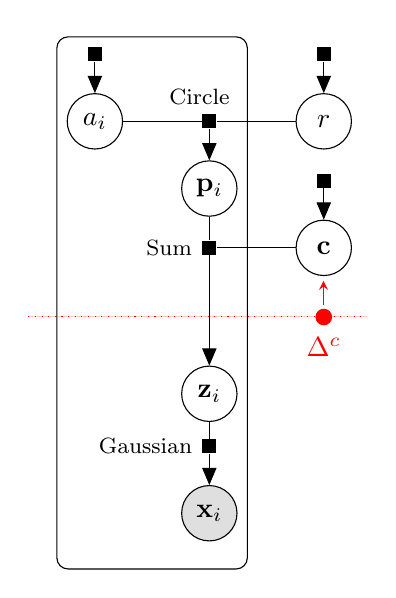
\begin{tikzpicture}

			\draw[red!20] (-2.3, 2.5) -- (2, 2.5);
			\draw[red, dotted] (-2.3, 2.5) -- (2, 2.5);

			\node[obs] 											(x)			{$\mathbf{x}_i$}; %
			\node[latent, above=of x, yshift=-2mm]                			(z)			{$\mathbf{z}_i$}; %

			\factor[above=of x]				 					{noise}		{left:Gaussian} {} {}; %
			\factor[above=of z, yshift=10mm] 					{sum}		{left:Sum} {} {}; %

			\node[latent, right=of sum]                			(c)			{$\mathbf{c}$}; %
			\node[latent, above=of sum, yshift=-7mm]   			(p)			{$\mathbf{p}_i$}; %

			\factor[above=of p] 								{circle}	{above:Circle\,\,\,\,\,} {} {}; %
			\factor[above=of c] 								{pc}		{} {} {}; %

			\node[latent, left=of circle]                		(a)			{$a_i$}; %
			\node[latent, right=of circle]                		(r)			{$r$}; %

			\factor[above=of a] 								{pa}		{} {} {}; %
			\factor[above=of r] 								{pr}		{} {} {}; %

			\factoredge {z} 		{noise} 		{x}; %
			\factoredge {p} 		{sum} 			{}; %
			\factoredge {a} 		{circle} 		{p}; %
			\factoredge {r} 		{circle} 		{}; %
			\factoredge {c} 		{sum} 			{z}; %
			\factoredge {} 			{pc} 			{c}; %
			\factoredge {} 			{pa} 			{a}; %
			\factoredge {} 			{pr} 			{r}; %

			\plate {} {(pa) (a) (p) (z) (x)} {}; %

			\fill (c.south) ++ (0, -0.52) circle (3pt) [fill=red] { };

			\draw [-stealth, red] (1.45, 2.65) -- (1.45, 2.95);

			\node[yshift=-0.9cm] at (c.south) { $\textcolor{red}{\Delta^c}$ };)

		\end{tikzpicture}
		\label{fig:circle-model}
	}
	\mycaption{The circle problem}{(a)~Given a sample of points on a circle (black), we wish to infer the circle's center (red) and its radius. Two sets of samples are shown. (b)~The graphical model for this problem.}
	\label{fig:circle}
\end{figure}

\begin{figure}[t]
	\centering
	\subfigure[Center]{
		\includegraphics[width=0.46\linewidth]{figures/Rotate4_Random_Center_Distance_10}
	}
	\subfigure[Radius]{
		\includegraphics[width=0.46\linewidth]{figures/Rotate4_Random_Radius_Distance_10}
	}
	\mycaption{Accelerated inference using \MTD for the circle problem}{(a)~Distance of the mean of the marginal posterior of center $c$ from its true value as a function of number of inference iterations (Forest: direct prediction, MP: standard VMP, \MTD: VMP with consensus). \Method significantly accelerates convergence. (b)~Similar plot for radius $r$. }
	\label{fig:circle-results}
\end{figure}

We begin by studying the behavior of standard message passing on a simplified Gauss and Ceres problem~\citep{Teets1999}.
Given a noisy sample of points $\obs = \{ \mathbf{x}_i \}_{i=1...N}$ on a circle in the 2D plane (Fig.~\ref{fig:circle-data}, black, $\mathcal{N}(0,0.01)$ noise on each axis), the aim is to infer the coordinates of the circle's center $\mathbf{c}$ (Fig.~\ref{fig:circle-data}, red) and its radius $r$. We can express the data generation process using a graphical model (Fig.~\ref{fig:circle-model}). The Cartesian point $(0, r)$ is rotated $a_i$ radians to generate $\mathbf{p}_i$, then translated by $\mathbf{c}$ to generate the latent $\mathbf{z}_i$, which finally produces the noisy observation $\mathbf{x}_i$.  This model can be expressed in a few lines of code in Infer.NET. The circle model is interesting for our purposes ,since it is both layered (the $\mathbf{z}_i$s, $\mathbf{p}_i$s and $a_i$s each form a layer) and loopy (due to the presence of two variables outside the plate).

We use this example to highlight the fact that although inference may require many iterations of message passing, message initialization can have a significant effect on the speed of convergence, and to demonstrate how this can be done automatically using \MTD.

Vanilla message passing inference in this model can take a surprisingly large number of iterations to converge. We draw 10 points $\{ \mathbf{x}_i \}$ from circles with random centers and radii, run VMP and record the accuracy of the marginals of the latent variables at each iteration. We repeat the experiment 50 times and plot results in Fig.~\ref{fig:circle-results} (dashed black). As can be seen from the figure, the marginals contain significant errors even after 50 iterations of message passing.

We then experiment with \method. A predictor $\Delta^c$ is trained to send a consensus message to $\mathbf{c}$ in the initial stages of inference, given the messages coming up from all of the $\mathbf{z}_i$ (indicated graphically in Fig.~\ref{fig:circle-model}, red). The predictor is trained on final beliefs at 100 iterations of standard message passing on $D=500$ sample problems.

As can be seen in Fig.~\ref{fig:circle-results} (red), this single consensus message has the effect of significantly increasing the rate of convergence (as indicated by slope) and also inference robustness (as indicated by error bars). For comparison, we also plot how well a regressor of the same capacity as the one used by \MTD can directly estimate the latent variables without using the graphical model in Fig.~\ref{fig:circle-results} (blue). \Method gives us the best of both worlds in this example: speed that is more comparable to one-shot bottom-up prediction and the accuracy of message passing inference in a good model for the problem.

\begin{figure}[t]
	\centering
	\subfigure[]{
		\setlength\fboxsep{-0.2mm}
		\setlength\fboxrule{0.7pt}
		\parbox[b]{2.3cm}{
			\fbox{\includegraphics[width=0.45\linewidth]{figures/Translate1_XData_1}} \hspace*{0mm}
			\fbox{\includegraphics[width=0.45\linewidth]{figures/Translate1_XData_2}} \vspace*{-2.4mm} \\
			\fbox{\includegraphics[width=0.45\linewidth]{figures/Translate1_XData_3}} \hspace*{0mm}
			\fbox{\includegraphics[width=0.45\linewidth]{figures/Translate1_XData_4}} \vspace*{-2.4mm} \\
			\fbox{\includegraphics[width=0.45\linewidth]{figures/Translate1_XData_5}} \hspace*{0mm}
			\fbox{\includegraphics[width=0.45\linewidth]{figures/Translate1_XData_6}} \vspace*{-2.4mm} \\
			\fbox{\includegraphics[width=0.45\linewidth]{figures/Translate1_XData_7}} \hspace*{0mm}
			\fbox{\includegraphics[width=0.45\linewidth]{figures/Translate1_XData_8}} \vspace*{-2.4mm} \\
			\fbox{\includegraphics[width=0.45\linewidth]{figures/Translate1_XData_9}} \hspace*{0mm}
			\fbox{\includegraphics[width=0.45\linewidth]{figures/Translate1_XData_10}} \vspace*{-2.4mm} \\
			\fbox{\includegraphics[width=0.45\linewidth]{figures/Translate1_XData_11}} \hspace*{0mm}
			\fbox{\includegraphics[width=0.45\linewidth]{figures/Translate1_XData_12}} \vspace*{-2.4mm} \\
			\fbox{\includegraphics[width=0.45\linewidth]{figures/Translate1_XData_13}} \hspace*{0mm}
			\fbox{\includegraphics[width=0.45\linewidth]{figures/Translate1_XData_14}}
		}
		\hspace{0.2cm}
		\label{fig:square-data}
	}
% 	\hfill
	\subfigure[]{
		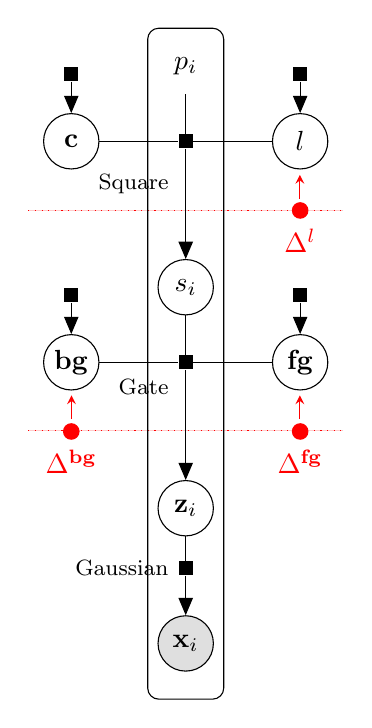
\begin{tikzpicture}

			\draw[red!20] (-2, 2.7) -- (2, 2.7);
			\draw[red, dotted] (-2, 2.7) -- (2, 2.7);

			\draw[red!20] (-2, 5.5) -- (2, 5.5);
			\draw[red, dotted] (-2, 5.5) -- (2, 5.5);

			\node[obs] 											(x)			{$\mathbf{x}_i$}; %
			\node[latent, above=of x]                			(z)			{$\mathbf{z}_i$}; %

			\factor[above=of x, yshift=1mm] 					{noise}		{left:Gaussian} {} {}; %
			\factor[above=of z, yshift=10mm] 					{gate}		{below left:Gate} {} {}; %

			\node[latent, right=of gate]                		(fg)		{$\mathrm{\mathbf{fg}}$}; %
			\node[latent, left=of gate]                			(bg)		{$\mathrm{\mathbf{bg}}$}; %
			\node[latent, above=of gate, yshift=-5mm]			(s)			{$s_i$}; %

			\factor[above=of s, yshift=10mm] 					{insq}		{below left, yshift=-2mm:Square} {} {}; %
			\factor[above=of fg] 								{pfg}		{} {} {}; %
			\factor[above=of bg] 								{pbg}		{} {} {}; %

			\node[latent, left=of insq]                			(c)			{$\mathbf{c}$}; %
			\node[latent, right=of insq]                		(l)			{$l$}; %
			\node[latent, above=of insq, yshift=-5mm, draw=none](p)			{$p_i$}; %

			\factor[above=of c] 								{pc}		{} {} {}; %
			\factor[above=of l] 								{pr}		{} {} {}; %

			\factoredge {z} 		{noise} 		{x}; %
			\factoredge {s} 		{gate} 			{z}; %
			\factoredge {c} 		{insq} 			{}; %
			\factoredge {l} 		{insq} 			{}; %
			\factoredge {p} 		{insq} 			{s}; %
			\factoredge {fg} 		{gate} 			{}; %
			\factoredge {bg} 		{gate} 			{}; %
			\factoredge {} 			{pfg} 			{fg}; %
			\factoredge {} 			{pbg} 			{bg}; %
			\factoredge {} 			{pc} 			{c}; %
			\factoredge {} 			{pr} 			{l}; %

			\plate {} {(p) (x)} {}; %

			\fill (bg.south) ++ (0, -0.52) circle (3pt) [fill=red] { };
			\fill (fg.south) ++ (0, -0.52) circle (3pt) [fill=red] { };

			\fill (l.south) ++ (0, -0.52) circle (3pt) [fill=red] { };

			\draw [-stealth, red] (-1.45, 2.85) -- (-1.45, 3.15);
			\draw [-stealth, red] (1.45, 2.85) -- (1.45, 3.15);

			\draw [-stealth, red] (1.45, 5.65) -- (1.45, 5.95);

			\node[yshift=-0.9cm] at (fg.south) { $\textcolor{red}{\Delta^{\mathrm{\mathbf{fg}}}}$ };
			\node[yshift=-0.9cm] at (bg.south) { $\textcolor{red}{\Delta^{\mathrm{\mathbf{bg}}}}$ };

			\node[yshift=-0.9cm] at (l.south) { $\textcolor{red}{\Delta^l}$ };)

		\end{tikzpicture}
		\hspace{0.1cm}
		\label{fig:square-model}
	}
	\mycaption{The square problem}{(a)~We wish to infer the square's center and its side length. (b)~A graphical model for this problem. $s_i$ is a boolean variable indicating the square's presence at position $p_i$. Depending on the value of $s_i$, the gate copies the appropriate color ($\mathrm{\mathbf{fg}}$ or $\mathrm{\mathbf{bg}}$) to $\mathbf{z}_i$.}
	\label{fig:square}
\end{figure}

\begin{figure}[t]
	\centering
	\subfigure[Center]{
		\includegraphics[width=0.4\linewidth]{figures/Translate4_Bullseye}
		\label{fig:square-results-bullseye}
	}
	\subfigure[Center]{
		\includegraphics[width=0.4\linewidth]{figures/Translate4_Center_Distance}
		\label{fig:square-results-center}
	}
	\subfigure[Side length]{
		\includegraphics[width=0.4\linewidth]{figures/Translate4_Radius_Distance}
		\label{fig:square-results-radius}
	}
	\subfigure[BG color]{
		\includegraphics[width=0.4\linewidth]{figures/Translate4_BGColor_Distance}
		\label{fig:square-results-bgcolor}
	}
	\mycaption{Robustified inference using \MTD for the square problem}{(a)~Position of inferred centers relative to ground-truth. Image boundaries shown in blue for scale. (b,c,d)~Distance of the mean of the posterior of $\mathbf{c}$, $l$ and $\mathrm{\mathbf{bg}}$ from their true values. \MTD consistently increases inference accuracy. Results have been averaged over 50 different problems. 1 stage \MTD only makes use of the lower predictors $\Delta^\mathrm{\mathbf{fg}}$ and $\Delta^\mathrm{\mathbf{bg}}$.}
	\label{fig:square-results}
\end{figure}


\subsection{A Generative Model of Squares}
\label{sec:square}

Next, we turn our attention to a more challenging problem for which even the best message passing scheme that we could devise frequently finds completely inaccurate solutions. The task is to infer the center $\mathbf{c}$ and side length $r$ of a square in an image (Fig.~\ref{fig:square-data}). Unlike the previous problem where we knew that all points belonged to the circle, here we must first determine which pixels belong to the square and which do not. To do so we might also wish to reason about the color of the foreground $\mathrm{\mathbf{fg}}$ and background $\mathrm{\mathbf{bg}}$, making the task of inference significantly harder. The graphical model for this problem is shown in Fig.~\ref{fig:square-model}. Let $\mathbf{c}$ and $l$ denote square center and side length respectively. At each pixel position $p_i$, $s_i$ is a boolean variable indicating the square's presence. Depending on the value of $s_i$, the gate copies the appropriate color ($\mathrm{\mathbf{fg}}$ or $\mathrm{\mathbf{bg}}$) to $\mathbf{z}_i$.

We experiment with 50 test images (themselves samples from the model), perform inference using EP and with a sequential schedule, recording the accuracy of the marginals of the latent variables at each iteration. We additionally place damping with step size 0.95 on messages from the square factor to the center $\mathbf{c}$. We found these choices led to the best performing standard message passing algorithm. Despite this, we observed inference accuracy to be disappointingly poor (see Fig.~\ref{fig:square-results}). In Fig.~\ref{fig:square-results-bullseye} we see that, for many images, message passing converges to highly inaccurate marginals for the center. The low quality of inference can also be seen in quantitative results of Figs.~\ref{fig:square-results}(b-d).

We implement \MTD predictors at two different layers of the model (see Fig.~\ref{fig:square-model}, red). In the first layer, $\Delta^\mathrm{\mathbf{fg}}$ and $\Delta^\mathrm{\mathbf{bg}}$ send consensus messages to $\mathrm{\mathbf{fg}}$ and $\mathrm{\mathbf{bg}}$ respectively, given the messages coming up from all of the $\mathbf{z}_i$ which take the form of independent Gaussians centered at the appearances of the observed pixels (we use a Gaussian noise model). Therefore $\Delta^\mathrm{\mathbf{fg}}$ and $\Delta^\mathrm{\mathbf{bg}}$ effectively make initial guesses of the values of the foreground and background colors in the image given the observed image. Split features in the internal nodes of the regression forest are designed to test for equality of two randomly chosen pixel positions, and sparse regressors are used at the leaves to prevent overfitting.

In the second layer, $\Delta^l$ sends a consensus message to $l$ given the messages coming up from all of the $s_i$. The messages from $s_i$ take the form of independent Bernoullis indicating the algorithm's current beliefs about the presence of the square at each pixel. Therefore, the predictor's job is to predict the square's side length from this probabilistic segmentation map. Note that it is much easier to implement a regressor to perform this task (effectively one only needs to count) than it is to do so using the original observed image pixels $x_i$. We find these predictors to be sufficient for stable inference and so we do not implement a fourth predictor for $\mathbf{c}$. We experiment with single stage \MTD, where only the lower predictors $\Delta^\mathrm{\mathbf{fg}}$ and $\Delta^\mathrm{\mathbf{bg}}$ are active, and with two stage \MTD, where all three predictors are active. The predictors are trained on $D=500$ samples from the model.

The results of these experiments are shown in Fig.~\ref{fig:square-results}. We observe that \MTD significantly improves the accuracy of inference for the center $\mathbf{c}$ (Figs.~\ref{fig:square-results-bullseye}, \ref{fig:square-results-center}) but also for the other latent variables (Figs.~\ref{fig:square-results-radius}, \ref{fig:square-results-bgcolor}). Note that single stage \MTD appears to be insufficient for guiding message passing to good solutions. Whereas in circle example \MTD accelerated convergence, this example demonstrates how it can make inference possible in models that were outside the capabilities of standard message passing.

\subsection{A Generative Model of Faces}
\label{sec:shading}

\begin{figure}[t]
	\centering
	\subfigure[]{
		\setlength\fboxsep{-0.3mm}
		\setlength\fboxrule{0pt}
		\parbox[b]{3cm}{
			\centering
			\small
			\fbox{\includegraphics[width=1.3cm]{figures/sample_N.png}}\\
			Normal $\{\mathbf{n}_i \}$ \vspace{4.5mm} \\
			\fbox{\includegraphics[width=1.3cm]{figures/sample_S.png}} \\
			Shading $\{ s_i \}$ \vspace{4.5mm} \\
			\fbox{\includegraphics[width=1.3cm]{figures/sample_R.png}} \\
			Reflectance $\{ r_i \}$ \vspace{4.5mm} \\
			\fbox{\includegraphics[width=1.3cm]{figures/sample_X.png}} \\
			Observed image $\{ x_i \}$\\
		}
		\hspace{0.1cm}
		\label{fig:shading-data}
	}
	% \hfill
	\subfigure[]{
		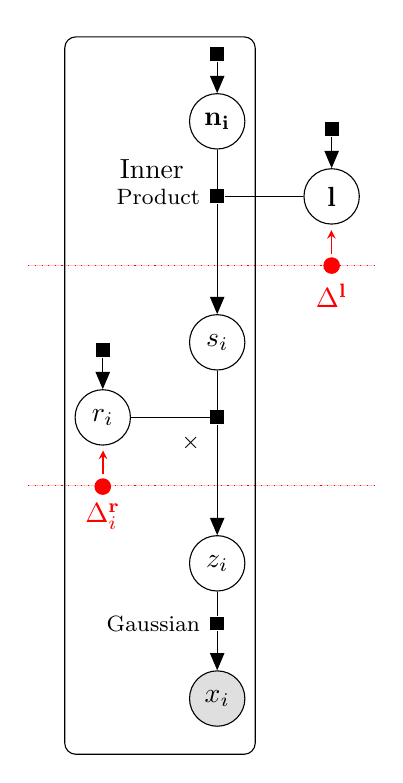
\begin{tikzpicture}

			\draw[red!20] (-2.4, 2.7) -- (2, 2.7);
			\draw[red, dotted] (-2.4, 2.7) -- (2, 2.7);

			\draw[red!20] (-2.4, 5.5) -- (2, 5.5);
			\draw[red, dotted] (-2.4, 5.5) -- (2, 5.5);

			\node[obs] 											(x)			{$x_i$}; %
			\node[latent, above=of x]                			(z)			{$z_i$}; %

			\factor[above=of z, yshift=10mm] 					{times}		{below left: $\times$} {} {}; %

			\node[latent, above=of times, yshift=-5mm]			(s)			{$s_i$}; %

			\factor[above=of x, yshift=1mm] 					{noise1}	{left:Gaussian} {} {}; %

			\node[latent, left=of times]                		(r)			{$r_i$}; %

			\factor[above=of r] 								{pr}		{} {} {}; %

			\factor[above=of s, yshift=10mm] 					{inner}		{left:Product} {} {}; %

			\node[latent, above=of inner, yshift=-5mm] 			(n)			{$\mathbf{n_i}$}; %
			\node[latent, right=of inner]                		(l)			{$\mathbf{l}$}; %

			\factor[above=of l] 								{pl}		{} {} {}; %

			\factor[above=of n] 								{pn}		{} {} {}; %

			\factoredge {z} 		{noise1} 		{x}; %
			\factoredge {s} 		{times} 		{z}; %
			\factoredge {r} 		{times} 		{}; %
			\factoredge {n} 		{inner} 		{s}; %
			\factoredge {l} 		{inner} 		{}; %
			\factoredge {} 			{pn} 			{n}; %
			\factoredge {} 			{pl} 			{l}; %
			\factoredge {} 			{pr} 			{r}; %

			\plate {} {(pn) (x) (r)} {}; %

			\fill (r.south) ++ (0, -0.52) circle (3pt) [fill=red] { };

			\fill (l.south) ++ (0, -0.52) circle (3pt) [fill=red] { };

			\draw [-stealth, red] (-1.45, 2.85) -- (-1.45, 3.15);

			\draw [-stealth, red] (1.45, 5.65) -- (1.45, 5.95);

			\node[yshift=-0.9cm] at (r.south) { $\textcolor{red}{\Delta_i^\mathbf{r}}$ };

			\node[yshift=-0.9cm] at (l.south) { $\textcolor{red}{\Delta^\mathbf{l}}$ };

			\node[yshift=0.35cm, xshift=-0.83cm] at (inner) { Inner };

		\end{tikzpicture}
		\label{fig:shading-model}
	}
	\mycaption{The face problem}{(a)~We observe an image and wish to infer the corresponding reflectance map and normal map (visualized here as 3D shape). (b)~A graphical model for this problem. Symmetry priors not shown.}
	\label{fig:shading}
	\vspace*{-4mm}
\end{figure}

In this sectin, we also investigate a more realistic application: face modeling. The estimation of reflectance and shape from a single image of a human face is a well-studied problem in computer vision (see \eg \citep{Georghiades2001, Lee2005, Wang2009, Kemelmacher2011, Tang2012}). A primary motivation for this task is that reflectance and shape are invariant to confounding light effects, and are therefore useful for downstream tasks such as recognition. The problem is ill-posed and modern approaches make use of prior knowledge in order to obtain good solutions, \eg in the form of average reflectance and normal statistics \citep{Biswas2009, Biswas2010} or morphable 3D models \citep{Zhang2006, Wang2009}.

\textbf{Model.} Given an observation of image pixels $\mathbf{x} = \{x_i\}$, the aim is to infer the reflectance value $r_i$ and normal vector $\mathbf{n_i}$ for each pixel $i$ (see Fig.~\ref{fig:shading-data}). In Fig.~\ref{fig:shading-model}, a model is shown for these variables that represents the following image formation process: $x_i = (\mathbf{n_i} \cdot \mathbf{l}) \times r_i + \epsilon$, thereby assuming Lambertian reflection and an infinitely distant directional light source with variable intensity. We place Gaussian priors over reflectances $\{ r_i \}$, normals $\{ \mathbf{n_i} \}$, and the light $\mathbf{l}$; and set the parameters of the priors using training data. We additionally place a soft symmetry prior on the $\{ r_i \}$ (the reflectance value on one side of the face should be close to its value on the other side) and on the $\{ \mathbf{n_i} \}$ (normal vectors on each side should be approximately symmetric), reflecting our prior knowledge about faces. These symmetry priors can be added to the model in just a few lines of code, illustrating the way in which model-based methods lend themselves to rapid prototyping and experimentation.

Although this model is only a crude approximation to the true image formation process (\eg it does not account for shadows or specularities), similar approximations have been found to be useful in prior work \citep{Biswas2009, Biswas2010, Kemelmacher2011}. Additionally, if we can successfully develop algorithms that perform accurate and reliable inference in this class of models, we would then be able to increase its usefulness by updating it to reflect the true image formation process more accurately. Note that even for a relatively small image of size $96 \times 84$, the model contains over 48,000 latent variables and 56,000 factors, and as we will show below, standard message passing in the model routinely fails to converge to accurate solutions.

\begin{figure*}
\begin{center}
\centerline{\includegraphics[width=1.0\columnwidth]{figures/face_cmp_visual_results.pdf}}
\vspace{-1.2cm}
\end{center}
	\mycaption{A visual comparison of inference results for the face problem}{For 4 randomly chosen test images, we show inference results obtained by competing methods. (a)~Observed images. (b)~Inferred reflectance maps. \textit{GT} is the stereo estimate which we use as a proxy for ground-truth, \textit{BU} is the bottom-up reflectance estimate of Biswas \etal (2009), \textit{MP} refers to standard variational message passing, \textit{Forest} is the consensus prediction and \textit{CMP} is the proposed consensus message passing technique. (c)~The variance of the inferred reflectance estimate produced by \MTD (normalized across rows). High variance regions correlate strongly with cast shadows. (d)~Visualization of inferred light. (e)~Inferred normal maps.}
	\label{fig:shading-qualitative-multiple-subjects}
\end{figure*}

\textbf{Consensus Message Passing.} We use predictors at two levels in the model (see Fig.~\ref{fig:shading-model}) to tackle this problem. The first sends consensus messages to \textit{each} reflectance pixel $r_i$, making it an instance of type B of \MTD as described in Fig.~\ref{fig:types-b}. Here, each consensus message is predicted using information from all the contextual messages from the $z_i$. We denote each of these predictors by $\Delta_i^\mathbf{r}$. The second predictor sends a consensus message to $\mathbf{l}$ using information from all the messages from the $s_i$ and is denoted by $\Delta^\mathbf{l}$. The first level of predictors effectively make a guess of the reflectance image from the denoised observation, and the second layer predictor produces an estimate of the light from the shading image (which is likely to be easier to do than directly from the observation). The reflectance predictors $\{ \Delta_i^\mathbf{r} \}$ are all powered by a single random forest, however the pixel position $i$ is used as a feature that it can exploit to create location specific behaviour. The tree parameterization of the contextual messages $\mathbf{c}$ for use in the reflectance predictor $\Delta_i^\mathbf{r}$ also includes 16 features such as mean, median, max, min and gradients of a $21 \times 21$ patch around the pixel. The tree parameterization of the contextual messages for use in the lighting predictor $\Delta^\mathbf{l}$ consists of means of the mean of the shading messages in $12 \times 12$ blocks. We deliberately use simple features to maintain generality but one could imagine the use of more specialized regressors for maximal performance.

\begin{figure}
	\centering
	\setlength\fboxsep{0.2mm}
	\setlength\fboxrule{0pt}
	\begin{tikzpicture}

		\matrix at (0, 0) [matrix of nodes, nodes={anchor=east}, column sep=-0.05cm, row sep=-0.2cm]
		{
			\fbox{\includegraphics[width=1cm]{figures/sample_3_1_X.png}} &
			\fbox{\includegraphics[width=1cm]{figures/sample_3_1_GT.png}} &
			\fbox{\includegraphics[width=1cm]{figures/sample_3_1_BISWAS.png}}  &
			\fbox{\includegraphics[width=1cm]{figures/sample_3_1_VMP.png}}  &
			\fbox{\includegraphics[width=1cm]{figures/sample_3_1_FOREST.png}}  &
			\fbox{\includegraphics[width=1cm]{figures/sample_3_1_CMP.png}}  &
			\fbox{\includegraphics[width=1cm]{figures/sample_3_1_CMPVAR.png}}
			 \\

			\fbox{\includegraphics[width=1cm]{figures/sample_3_2_X.png}} &
			\fbox{\includegraphics[width=1cm]{figures/sample_3_2_GT.png}} &
			\fbox{\includegraphics[width=1cm]{figures/sample_3_2_BISWAS.png}}  &
			\fbox{\includegraphics[width=1cm]{figures/sample_3_2_VMP.png}}  &
			\fbox{\includegraphics[width=1cm]{figures/sample_3_2_FOREST.png}}  &
			\fbox{\includegraphics[width=1cm]{figures/sample_3_2_CMP.png}}  &
			\fbox{\includegraphics[width=1cm]{figures/sample_3_2_CMPVAR.png}}
			 \\

			\fbox{\includegraphics[width=1cm]{figures/sample_3_3_X.png}} &
			\fbox{\includegraphics[width=1cm]{figures/sample_3_3_GT.png}} &
			\fbox{\includegraphics[width=1cm]{figures/sample_3_3_BISWAS.png}} &
			\fbox{\includegraphics[width=1cm]{figures/sample_3_3_VMP.png}}  &
			\fbox{\includegraphics[width=1cm]{figures/sample_3_3_FOREST.png}}  &
			\fbox{\includegraphics[width=1cm]{figures/sample_3_3_CMP.png}}  &
			\fbox{\includegraphics[width=1cm]{figures/sample_3_3_CMPVAR.png}}
			 \\
	     };


	     \node at (-3.85, -2.0) {\small Observed};
	     \node at (-2.55, -2.0) {\small `GT'};
	     \node at (-1.27, -2.0) {\small BU};
	     \node at (0.0, -2.0) {\small MP};
	     \node at (1.27, -2.0) {\small Forest};
	     \node at (2.55, -2.0) {\small \textbf{CMP}};
	     \node at (3.85, -2.0) {\small Variance};

	\end{tikzpicture}
	\mycaption{Robustness to varying illumination}{Left to right: observed image, photometric stereo estimate (proxy for ground-truth), \cite{Biswas2009} estimate, VMP result, consensus forest estimate, CMP mean, and CMP variance.}
	\label{fig:shading-qualitative-same-subject}
  \vspace{-0.3cm}
\end{figure}

\begin{figure}[t]
	\centering
	\subfigure[Without shadows]{
		\includegraphics[width=0.4\linewidth]{figures/Shading_Recognition_Rate_Synthetic}
	}
	\subfigure[With shadows]{
		\includegraphics[width=0.4\linewidth]{figures/Shading_Recognition_Rate_Real}
	}
	\mycaption{Reflectance inference accuracy demonstrated through recognition accuracy}{\MTD allows us to make use of the full potential of the generative model, thereby outperforming the competitive bottom-up method of \cite{Biswas2009}.}
	\label{fig:shading-quantitative-reflectance}

	\subfigure[Without shadows]{
		\includegraphics[width=0.4\linewidth]{figures/Shading_Light_Angle_Error_Synthetic}
	}
	\subfigure[With shadows]{
		\includegraphics[width=0.4\linewidth]{figures/Shading_Light_Angle_Error_Real}
	}
	\mycaption{Light inference accuracy}{The presence of cast shadows makes the direct prediction task easier, however \MTD is accurate even in their absence.}
	\label{fig:shading-quantitative-light}
\end{figure}

\textbf{Datasets.} We experiment with the `Yale B' and `Extended Yale B' datasets~\citep{Georghiades2001, Lee2005}. Together, they contain images of 38 subjects each with 64 illumination directions. We remove images taken with extreme light angles (azimuth or elevation $\ge 85$ degrees) that are almost entirely in shadow, leaving around 45 images for each subject. Images are down-sampled to $96 \times 84$. There are no ground-truth normals or reflectances for this dataset, however it is common practice to create proxy ground-truths using photometric stereo, which we obtain using the code of~\cite{Queau2013}. We use images from 22 subjects for training and test on the remaining 16 subjects.

\textbf{Results.} We begin by qualitatively assessing the different inference schemes. In Fig.~\ref{fig:shading-qualitative-multiple-subjects} we show inference results for reflectance maps, normal maps and lights that are obtained after 100 iterations of message passing (VMP). For reflectance (Fig.~\ref{fig:shading-qualitative-multiple-subjects}b), we would like inference to produce estimates that match closely the ground-truth produced by photometric stereo (GT). We also display the reflectance estimates produced by the strong baseline (BU) of \cite{Biswas2009} for reference. We note that the baseline achieves excellent accuracy in regions with strong lighting, however it produces blurry estimates in regions under shadow.

As can be seen in Fig.~\ref{fig:shading-qualitative-multiple-subjects}b (MP), standard variational message passing finds solutions that are highly inaccurate with continued presence of illumination and artifacts in areas of cast show. In contrast, inference using \MTD produces artefact-free results that much more closely resemble the stereo ground-truths. Arguably \MTD also improves over the baseline \citep{Biswas2009}, since its estimates are not blurry in regions with cast shadows. This can be attributed to the presence of symmetry priors in the model. Additionally, we note that the variance of the \MTD inference for reflectance (Fig.~\ref{fig:shading-qualitative-multiple-subjects}c) correlates strongly with cast shadows in the observed images (\ie the model is uncertain where it should be) suggesting that in future work it would be fruitful to have the notion of cast shadows explicitly built into the model. Figs.~\ref{fig:shading-qualitative-multiple-subjects}d and \ref{fig:shading-qualitative-multiple-subjects}e show analogous results for lighting and normal maps, and Fig.~\ref{fig:shading-qualitative-same-subject} demonstrates \MTD's ability to robustly infer reflectance maps for images of a single subject taken under varying lighting conditions. More visual results are shown in the supplementary at the end of this thesis
(Figs.~\ref{fig:shading-qualitative-multiple-subjects-supp},~\ref{fig:shading-qualitative-same-subject}).

We use the task of subject recognition (using estimated reflectance) as a quantitative measure of inference accuracy, as it can be difficult to measure in more direct ways (\eg RMSE strongly favors blurry predictions). The reflectance estimate produced by each algorithm is compared to all training subjects' ground-truth reflectances and is assigned the label of its closest match. We have found this evaluation to reflect the quality of inference estimates. Fig.~\ref{fig:shading-quantitative-reflectance} shows the result of this experiment, both for real images and also synthetic images that were produced by taking the stereo ground-truths and adding artificial lighting (but with no cast shadows). We show analogous results for light in Fig.~\ref{fig:shading-quantitative-light}, where error is defined to be the cosine angle distance between the estimated light and the photometric stereo reference. First, we note that standard variational message passing (MP) performs poorly, producing reflectance estimates that are much less useful for recognition than those from \cite{Biswas2009}. Second, we note that \MTD in the same model (both 1 stage and 2 stage versions) produces inferences that are significantly more useful downstream. The horizontal line labelled `Forest' represents the accuracy of the consensus messages without any message passing, showing that the model-based fine-tuning provides a significant benefit. Finally, we highlight the fact that initializing light directly from the image and running message passing (Fig.~\ref{fig:shading-quantitative-reflectance}, Init+MP) leads to worse estimates than \MTD demonstrating the use of layered predictions as opposed to direct predictions from the observations. These results demonstrate that \MTD helps message passing find better fixed points even in the presence of model mis-match (shadows) and make use of the full potential of the generative model.

\section{Discussion and Conclusions}
\label{sec:discussion-chap4}

We have presented \METHOD and shown that it is a computationally efficient technique that can be used to improve the accuracy of message passing inference in a variety of vision models. The crux of the approach is to recognize the importance of global variables, and to take advantage of layered model structures commonly seen in vision to make rough estimates of their values.

The success of \MTD depends on the accuracy of the random forest predictors. The design of forest features is not yet completely automated, but we took care in this work to use generic features that can be applied to a broad class of problems. Our forests are implemented in an extensible manner, and we envisage building a library of them that one can choose from, simply by inspecting the data types of the contextual and target variables.

In future work, we would like to exploit the benefits of the \MTD framework by applying it to more challenging problems from computer vision. Each of the examples in Section~\ref{sec:experiments-chap4} can be extended in various ways, \eg by making considerations for multiple objects, incorporating occlusion in the squares example and cast shadows in the faces example, or by developing more realistic priors. We are also seeking to understand in what other domains the application of our ideas may be fruitful.

More broadly, a major challenge in machine learning is that of enriching models in a scalable way. We continually seek to ask our models to provide interpretations of increasingly complicated, heterogeneous data sources. Graphical models provide an appealing framework to manage this complexity, but the difficulty of inference has long been a barrier to achieving these goals. The \MTD framework takes us one step in the direction of overcoming this barrier.


\part{Inference in Discriminative Vision Models}
\section{Summary and future work}


We have presented techniques for scaling and squaring algorithms that
allow for the incremental computation of block triangular matrix
exponentials.  We combined these techniques with an adaptive scaling
strategy that allows for both fast and accurate computation of each
matrix exponential in this sequence (Algorithm~\ref{alg:adaptive}).
For our application in polynomial diffusion models, the run time can
be further reduced by using fixed scaling parameter, determined
through the estimation techniques in Lemmas~\ref{lemmanormJ}
and~\ref{lem:heston_est}.

We observed in our numerical experiments that accurate approximations
to these matrix exponentials can be obtained even for quite small,
fixed scaling parameters.  For the case of two-by-two block triangular
matrices, the results of Dieci and Papini~\cite{Dieci2000,Dieci2001}
support this finding, but an extension of these results to cover a
more general setting would be appreciable.





\chapter{Video Propagation Networks}
\label{chap:vpn}

In this chapter, we leverage the learnable bilateral filters developed in the
previous chapter, and develop a novel neural network architecture for inference
in video data. We focus on the task of propagating information across video
frames. Standard CNNs are poor candidates for filtering video data.
Standard spatial CNNs have fixed receptive fields whereas the video content
changes differently in different videos depending on the type of scene and camera
motion. So, filters with video adaptive receptive fields are better candidates
for video filtering.

Based on this observation, we adapt the bilateral convolution layers (BCL) proposed
in the previous chapter for filtering video data.
By stacking several BCL and standard spatial convolutional
layers, we develop a neural network architecture for video information propagation
which we call `Video Propagation Network' (VPN). We evaluate VPN on different
tasks of video object segmentation and semantic video segmentation
and show increased performance comparing to the best previous task-specific methods,
while having favorable runtime. Additionally we demonstrate our approach on an example
regression task of propagating color in a grayscale video.

\section{Introduction}

% Why information propagation in videos?
We focus on the problem of propagating structured information across video frames in this chapter.
~This problem appears in many forms (e.g., semantic segmentation or depth estimation) and is a pre-requisite for many applications.~An example instance is shown in Fig.~\ref{fig:illustration-vpn}.
Given an accurate object mask for the first frame, the problem is to propagate this mask forward
through the entire video sequence.~Propagation of semantic information through time and video
colorization are other problem instances.

% What are the main challenges?
Videos pose both technical and representational challenges.
The presence of scene and camera motion lead to the difficult association problem of optical flow.
Video data is computationally more demanding than static images. A naive per-frame approach would scale at least linear with frames.
These challenges complicate the use of standard convolutional neural networks (CNNs) for video processing.
As a result, many previous works for video propagation use slow optimization based techniques.


\begin{figure}[t!]
\begin{center}
\centerline{\includegraphics[width=\columnwidth]{figures/teaser_network.pdf}}
  \mycaption{Video Propagation with VPNs} {The end-to-end trained VPN network is composed
  of a bilateral network followed by a standard spatial network and can be used for
  propagating information across frames. Shown here is an example result
  of foreground mask from the 1$^{st}$ frame to other video frames.}
  \label{fig:illustration-vpn}
  \vspace{-0.3cm}
\end{center}
\end{figure}

% What we do in this work? And also briefly about VPNs
We propose a generic neural network architecture that propagates information across
video frames. The main innovation is the use of image adaptive convolutional operations that automatically
adapt to
the video stream content.~This allows the network to adapt to the changing content of the video stream.
It can be applied to several types of information, e.g. labels, colors, etc. and runs online, that is, only requiring current and previous frames.

% Briefly about VPNs
Our architecture is composed of two components (see Fig.~\ref{fig:illustration-vpn}).
A temporal \textit{bilateral network} that performs image-adaptive spatio-temporal dense filtering.
This part allows to connect densely all pixels from current and previous frames and to propagate associated pixel information to the current frame.
The bilateral network allows the specification of a metric between video pixels and allows a straight-forward integration of temporal information.
This is followed by a standard \textit{spatial CNN} on the filter output to refine and predict for the present video frame.
We call this combination a \textit{Video Propagation Network (VPN)}.
In effect we are combining a filtering technique with rather small spatial CNNs which leads to a favorable runtime compared to many previous approaches.

VPNs have the following suitable properties for video processing:

\vspace{-0.5cm}
\paragraph{General applicability:} VPNs can be used for propagating any
type of information content i.e., both discrete
(e.g., semantic labels) and continuous (e.g. color) information across video frames.
\vspace{-0.5cm}
\paragraph{Online propagation:} The method needs no future frames
and so can be used for online video analysis.
\vspace{-0.5cm}
\paragraph{Long-range and image adaptive:} VPNs can efficiently handle a large
number of input frames and are adaptive to the video.
\vspace{-0.5cm}
\paragraph{End-to-end trainable:} VPNs can be trained end-to-end, so they
can be used in other deep network architectures.
\vspace{-0.5cm}
\paragraph{Favorable runtime:} VPNs have favorable runtime in comparison to several current
best methods, also making them amenable for learning with
large datasets.

Empirically we show that VPNs, despite being generic,
perform better or on-par with current best approaches on video object segmentation
and semantic label propagation while being faster.
VPNs can easily be integrated into sequential per-frame approaches
and require only a small fine-tuning step that can be performed separately.

\section{Related Work}
\label{sec:related}

The literature on propagating information across video frames contains a vast and varied number of approaches.
Here, we only discuss those works that are related to our technique and applications.

\vspace{-0.3cm}
\paragraph{General propagation techniques}
Techniques for propagating content across
image or video pixels are predominantly
optimization based or filtering techniques. Optimization
based techniques typically formulate the propagation as an energy minimization problem
on a graph constructed across video pixels or frames.
A classic example is the color propagation technique from~\cite{levin2004colorization} which uses
graph structure that encodes prior knowledge about pixel colors in a local neighborhood.
Although efficient closed-form
solutions~\cite{levin2008closed} exists for certain scenarios,
optimization tends to be slow due to either large graph structures for videos and/or the use of
complex connectivity resulting in the use of iterative optimization schemes. Fully-connected conditional
random fields (CRFs)~\cite{krahenbuhl2012efficient} open a way for incorporating dense
and long-range pixel connections while retaining fast inference.

Filtering techniques~\cite{kopf2007joint,chang2015propagated,he2013guided} aim to propagate
information with the use of image or video filters resulting in fast runtimes compared
to optimization techniques. Bilateral filtering~\cite{aurich1995non,tomasi1998bilateral} is
one of the popular filters for long-range information propagation.
We have already discussed bilateral filtering and its generalization in the previous
chapter. A popular application, that is also discussed in previous chapter, is joint
bilateral up-sampling~\cite{kopf2007joint} that up-samples a low-resolution signal with
the use of a high-resolution guidance image.
Chapter~\ref{chap:bnn} and the works
of~\cite{li2014mean,domke2013learning,zheng2015conditional,schwing2015fully,barron2015bilateral}
showed that one can back-propagate through the bilateral filtering operation for
learning filter parameters (Chapter~\ref{chap:bnn}) or doing optimization in the bilateral
space~\cite{barron2015bilateral,barron2015defocus}.
Recently, several works proposed to do upsampling
in images by learning CNNs that mimics edge-aware filtering~\cite{xu2015deep} or
that directly learns to up-sample~\cite{li2016deep,hui2016depth}.
Most of these works are confined to images and are either not extendible or computationally
too expensive for videos. We leverage some of these previous works and propose a
scalable yet robust neural network based approach for video content propagation.

\vspace{-0.3cm}
\paragraph{Video object segmentation}

Prior work on video object segmentation can be broadly categorized into two types:
Semi-supervised methods that require manual annotation to define what is foreground
object and unsupervised methods that does segmentation completely automatically.
Unsupervised techniques such as
~\cite{faktor2014video,li2013video,lee2011key,papazoglou2013fast,wang2015saliency,
zhang2013video,taylor2015causal,dondera2014interactive}
use some prior information about the foreground objects such as
distinctive motion, saliency etc. And, they typically fail if these
assumptions do not hold in a video.

In this work, we focus on the semi-supervised task of propagating the foreground
mask from the first frame to the entire video. Existing works
predominantly use graph-based optimization frameworks that perform graph-cuts~\cite{boykov2001fast,
boykov2001interactive,shi2000normalized} on video data.
Several of these works~\cite{reso2014interactive,
li2005video,price2009livecut,wang2005interactive,kohli2007dynamic,jain2014supervoxel}
aim to reduce the complexity of graph structure with
clustering techniques such as spatio-temporal superpixels and
optical flow~\cite{tsaivideo}.
Another direction was to estimate correspondence between different frame
pixels~\cite{agarwala2004keyframe,bai2009video,lang2012practical} by using
nearest neighbor fields~\cite{fan2015jumpcut} or optical flow~\cite{chuang2002video}
and then refine the propagated masks with the use of local classifiers.
Closest to our technique are the works of~\cite{perazzi2015fully} and~\cite{marki2016bilateral}.
~\cite{perazzi2015fully} proposed to use fully-connected CRF over the
refined object proposals across the video frames.~\cite{marki2016bilateral} proposed a
graph-cut in the bilateral space. Our approach is similar in the regard that we also
use a bilateral space embedding. Instead of graph-cuts, we learn
propagation filters in the high-dimensional bilateral space with CNNs.
This results in a more generic architecture and allows integration into other deep learning frameworks.

Two contemporary works~\cite{caelles2016one,khoreva2016learning} proposed CNN based
approaches for video object segmentation. Both works rely on fine-tuning a deep network
using the first frame annotation of a given test sequence. This could potentially result
in overfitting to the background.
In contrast, the proposed approach relies only on offline training and thus can be easily adapted
to different problem scenarios.

\vspace{-0.3cm}
\paragraph{Semantic video segmentation}
Earlier methods such as~\cite{brostow2008segmentation,sturgess2009combining} use structure from motion
on video frames to compute geometrical and/or motion features.
More recent works~\cite{ess2009segmentation,chen2011temporally,de2012line,miksik2013efficient,tripathi2015semantic,
kundu2016feature} construct large graphical models on videos and enforce temporal consistency across frames. \cite{chen2011temporally} used dynamic temporal links in their CRF energy formulation.
\cite{de2012line} proposes to use Perturb-and-MAP random field model with spatio-temporal energy terms
based on Potts model and \cite{miksik2013efficient} propagate predictions across time by learning
a similarity function between pixels of consecutive frames.

In the recent years, there is a big leap in the performance of semantic image
segmentation~\cite{long2014fully,chen2014semantic} with the use of CNNs but mostly
applied to images. Recently,~\cite{shelhamer2016clockwork}
proposed to retain the intermediate CNN representations while sliding the image based
CNN across the frames. Another approach, which inspired our work, is to take unary
predictions from CNN and then propagate semantic information across the frames. A recent
prominent approach in this direction is of~\cite{kundu2016feature} which proposes
a technique for optimizing feature spaces for fully-connected CRF.

\section{Video Propagation Networks}
\label{sec:vpn}

We aim to adapt the bilateral filtering operation to predict information forward in time, across video frames.
Formally, we work on a sequence of $n$ (color or grayscale) images $\obs = \{\obs_1, \obs_2, \cdots, \obs_n\}$
and denote with $\target = \{\target_1, \target_2, \cdots, \target_n\}$ a sequence of outputs, one per frame.
Consider as an example, a sequence $\target_1,\ldots,\target_n$ of foreground masks for a moving object in the
scene. Our goal is to develop an online propagation method, that is, a function that has no access to the future frames.
Formally we predict $\target_t$, having observed the video up to frame $t$ and possibly previous $\target_{1,\cdots,t-1}$
\begin{equation}
\mathcal{F}(\target_{t-1}, \target_{t-2}, \cdots; \obs_t, \obs_{t-1}, \obs_{t-2},\cdots) = \target_t.
\end{equation}

\begin{figure*}[t!]
\begin{center}
\centerline{\includegraphics[width=\textwidth]{figures/net_illustration.pdf}}
  \mycaption{Computation Flow of Video Propagation Network} {Bilateral networks (BNN) consist of a series of bilateral filterings interleaved with ReLU non-linearities. The filtered information from BNN is then passed into a spatial network (CNN) which refines the features with convolution layers interleaved with ReLU
  non-linearities, resulting in the prediction for the current frame.}
  \label{fig:net_illustration}
\end{center}
\end{figure*}


If training examples $(\obs,\target)$ with full or partial knowledge of $\target$ are available, it is possible to learn $\mathcal{F}$ and for a complex and unknown relationship between input and output, a deep CNN is a natural design
choice. However, any learning based method has to face the main challenge: the scene and camera motion and its
effect on $\target$. Since no motion in two different videos is the same, fixed-sized static receptive fields of CNN units are insufficient.
We propose to resolve this with video-adaptive convolutional component, an adaption of the bilateral filtering to videos.
Our Bilateral Network (Section~\ref{sec:bilateralnetwork}) has a connectivity that adapts to video sequences, its output is then fed into a common Spatial Network (Section~\ref{sec:spatialcnn}) that further refines the desired output.
The combined network layout of this Video Propagation Network is depicted in Fig.~\ref{fig:net_illustration}.
It is a sequence of learnable bilateral and spatial filters that is efficient, trainable end-to-end and adaptive to the video input.

\begin{figure*}[t!]
\begin{center}
  \centerline{\includegraphics[width=\textwidth]{figures/permutohedral_illustration_2.pdf}}
    \mycaption{Schematic of Fast Bilateral Filtering for Video Processing}
    {Mask probabilities from previous frames $V_{1,\cdots,t-1}$ are splatted on to the
    lattice positions defined by the image features $f_{I_{1}},f_{I_2},\cdots,f_{I_{t-1}}$.
    The splatted result is convolved with a $1 \times 1$ filter $B$, and the filtered
    result is sliced back to the original image space to get $V_t$ for the present frame.
    Input and output need not be $V_t$, but can also be an intermediate neural network representation.
    $B$ is learned via back-propagation through these operations.}
    \label{fig:filter_illustration}
\end{center}
\end{figure*}

\subsection{Bilateral Network (BNN)}\label{sec:bilateralnetwork}
In this section, we describe the extension of the learnable bilateral filtering, proposed in
Chapter~\ref{chap:bnn} to video data.
Several properties of bilateral filtering make it a perfect candidate for information propagation in videos.
In particular, our method is inspired by two main ideas that we extend in this work: joint bilateral up-sampling~\cite{kopf2007joint} and learnable bilateral filters (Chapter~\ref{chap:bnn}). Although,
bilateral filtering has been used for filtering video data before~\cite{paris2008edge},
its use has been limited to fixed filter weights (say, Gaussian).

{\bf Fast Bilateral Up-sampling across Frames} The idea of joint bilateral up-sampling~\cite{kopf2007joint}
is to view up-sampling as a filtering operation.
A high resolution guidance image is used to up-sample a low-resolution result.
In short, a smaller number of input points $\target_i$ and the corresponding features $\f_i$
are given $\target_i,\f_i; i=1,\ldots,N_{in}$, for example a segmentation result $\target_i$ at a lower resolution.
This is then scaled to a larger number of output points $\f_j;j=1,\ldots,N_{out}$ using the
bilateral filtering operation, that is to compute the following bilateral filtering equation:

\begin{equation}
  \target'_i = \sum_{j=1}^n \bw_{\f_i,\f_j} \target_j
  \label{eq:bilateral2}
\end{equation}

where the sum runs over all $N_{in}$ points and the output is computed for all $N_{out}$ positions.
We will use this idea to propagate content from previous frames to the current frame (all of which have the same dimensions), using the current frame as a guidance image.
This is illustrated in Fig.~\ref{fig:filter_illustration}. We take all previous frame results $\target_{1,\cdots,t-1}$
 and splat them into a lattice using the features computed on video frames $\obs_{1,\cdots,t-1}$.
A filtering (described below) is applied to every lattice point and the result is then sliced back using the
current frame $\obs_t$.
This result need not be the final $\target_t$, in fact we compute a filter bank of responses and continue with further
processing as will be discussed.

For videos, we need to extend bilateral filtering to temporal data, and there are two natural choices.
First, one can simply attach a frame index $t$ as an additional time dimension to the input data, yielding a six dimensional feature vector $\f=(x,y,r,g,b,t)^{\top}$ for every pixel in every frame.
The summation in Eq.~\ref{eq:bilateral2} now runs over \emph{all} previous frames and pixels.
Imagine a video where an object moves to reveal some background.
Pixels of the object and background will be close spatially $(x,y)$ and temporally $(t)$ but likely be of different color $(r,g,b)$.
Therefore they will have no strong influence on each other (being splatted to distant positions in the six-dimensional bilateral space).
In summary, one can understand the filter to be adaptive to color changes across frames, only pixels that are static and have similar color have a strong influence on each other (end up nearby in the lattice space).
The second possibility is to use optical flow. If the perfect flow is available, the video frames could be warped into a common frame of reference. This would resolve the corresponding problem and make information propagation much easier.
We can make use of an optical flow estimate by warping pixel positions $(x,y)$ by their displacement vector $(u_x,u_y)$ to $(x+u_x,y+u_y)$.

Another property of permutohedral filtering that we exploit
is that the \emph{inputs points need not lie on a regular grid} since the filtering
is done in the high-dimensional lattice. Instead of splatting millions of pixels on to the
lattice, we randomly sample or use superpixels and perform filtering using these sampled
points as input to the filter. In practice, we observe that this results in big computational
gains with minor drop in performance (more in Sec.~\ref{sec:videoseg}).

{\bf Learnable Bilateral Filters} The property of propagating information forward using a guidance image through filtering solves the problem of pixel association.
But a Gaussian filter may be insufficient and further, we would like to increase the capacity by using a filter bank instead of a single fixed filter.
We propose to use the technique proposed in previous chapter
to learn the filter values in the permutohedral lattice using back-propagation.

The process works as follows.
A input video is used to determine the positions in the bilateral space to splat the input points
$\target(i)\in\mathbb{R}^D$ i.e. the features $\f$ (e.g. $(x,y,r,g,b,t)$) define the splatting matrix $S_{splat}$.~This leads to a number of vectors $\target_{splatted} = S_{splat}\target$, that lie on the permutohedral lattice, with dimensionality $\target_{splatted}\in\mathbb{R}^D$.
In effect, the splatting operation groups points that are close together, that is, they have similar $\f_i,\f_j$.
All lattice points are now filtered using a filter bank $B\in\mathbb{R}^{F\times D}$ which results in $F$ dimensional vectors on the lattice points.
These are sliced back to the $N_{out}$ points of interest (present video frame).
The values of $B$ are learned by back-propagation.
General parameterization of $B$ from previous chapter allows to have
any neighborhood size for the filters. Since constructing the neighborhood structure in
high-dimensions is time consuming, we choose to use $1 \times 1$ filters for speed reasons.
This makes up one \emph{Bilateral Convolution Layer (BCL)} which we will stack and concatenate to form a Bilateral Network. See Fig.~\ref{fig:filter_illustration} for an illustration of a BCL.

{\bf BNN Architecture} The Bilateral Network (BNN) is illustrated in the green box of
Fig.~\ref{fig:net_illustration}.
The input is a video sequence $\obs$ and the corresponding predictions $\target$ up to frame
$t$. Those are filtered using two BCLs with $32$ filters each.
For both BCLs, we use the same features $\f$ but scale them with different diagonal matrices
$\f_a=\Lambda_a\f,\f_b=\Lambda_b\f$. The feature scales are found by cross-validation.
The two $32$ dimensional outputs are concatenated, passed through a ReLU non-linearity and passed to a
second layer of two separate BCL filters that uses same feature spaces $\f_a,\f_b$.
The output of the second filter bank is then reduced using a $1\times 1$ spatial filter (C-1) to map to
the original dimension of $\target$.
We investigated scaling frame inputs with an exponential time decay and found that, when processing
frame $t$, a re-weighting with $(\alpha \target_{t-1}, \alpha^2 \target_{t-2}, \alpha^3 \target_{t-3} \cdots)$ with
$0\le\alpha\le 1$ improved the performance a little bit.

In the experiments, we also included a simple BNN variant,
where no filters are applied inside the permutohedral space, just splatting and slicing
with the two layers $BCL_a$ and $BCL_b$ and adding the results.
We will refer to this model as \emph{BNN-Identity},
it corresponds to an image adaptive smoothing of the inputs $\target$.
We found this filtering to have a positive effect and include it as a baseline in our experiments.

\vspace{-0.1cm}
\subsection{Spatial Network}\label{sec:spatialcnn}

The BNN was designed to propagate the information from the previous frames, respecting the scene and object motion.
We then add a small spatial CNN with 3 layers, each with $32$ filters of size $3\times 3$,
interleaved with ReLU non-linearities.
The final result is then mapped to the desired output of $\target_t$ using a $1\times 1$
convolution.
The main role of this spatial CNN is to refine the information in frame $t$.
Depending on the problem and the size of the available training data, other network designs are
conceivable. We use the same network architecture shown in Fig.~\ref{fig:net_illustration}
for all the experiments to demonstrate the generality of VPNs.

\vspace{-0.1cm}
\section{Experiments}
\label{sec:exps}

We evaluated VPN on three different propagation tasks: foreground masks, semantic
labels and color information in videos. Our implementation runs in Caffe~\cite{jia2014caffe} using standard settings. We used Adam~\cite{kingma2014adam} stochastic optimization for training VPNs, multinomial-logistic loss for label propagation networks and Euclidean loss for training
color propagation networks. Runtime computations were performed using a
Nvidia TitanX GPU and a 6 core Intel i7-5820K CPU clocked at 3.30GHz machine.
We will make available all the code and experimental results.

\subsection{Video Object Segmentation}
\label{sec:videoseg}

The task of class-agnostic video object segmentation aims to segment foreground objects in
videos. Since the semantics of the foreground object is not pre-defined, this problem is
usually addressed in a semi-supervised manner. The goal is to propagate a
given foreground mask of the first frame to the entire video frames.
Object segmentation in videos is useful for several high level tasks such
as video editing, summarization, rotoscoping etc.

\vspace{-0.5cm}
\paragraph{Dataset} We use the recently published DAVIS dataset~\cite{Perazzi2016}
for experiments on this task. The
DAVIS dataset consists of 50 high-quality (1080p resolution) unconstrained videos
with number of frames in each video ranging from 25 to 104. All the frames come with
high-quality per-pixel annotation of the foreground object. The videos for this
dataset are carefully chosen to contain motion blur, occlusions, view-point changes
and other occurrences of object segmentation challenges.
For robust evaluation and to get results on all the dataset videos,
we evaluate our technique using 5-fold cross-validation.
We randomly divided the data into
5 folds, where in each fold, we used 35 images for training, 5 for validation and
the remaining 10 for the testing. For the evaluation, we used the 3 metrics that
are proposed in~\cite{Perazzi2016}: Intersection over Union (IoU) score, Contour
accuracy ($\mathcal{F}$) score and temporal instability ($\mathcal{T}$) score. The widely
used IoU score is defined as $TP/(TP+FN+FP)$, where TP: True positives; FN: False negatives
and FP: False positives. Please refer to~\cite{Perazzi2016} for the definition of the contour
accuracy and temporal instability scores. We are aware of some other datasets for
this task such as JumpCut~\cite{fan2015jumpcut} and
SegTrack~\cite{tsai2012motion}, but we note that the number of videos in these datasets is too
small for a learning based approach.

\begin{table}[t]
    % \scriptsize
    % \fontsize{5}{3.2}\selectfont
    \centering
    \begin{tabular}{p{3.0cm}>{\centering\arraybackslash}p{1.2cm}>{\centering\arraybackslash}
      p{1.2cm}>{\centering\arraybackslash}p{1.2cm}>{\centering\arraybackslash}p{1.2cm}>{\centering\arraybackslash}p{1.2cm}
      >{\centering\arraybackslash}p{0.6cm}}
        \toprule
        \scriptsize
        & Fold-1 & Fold-2 & Fold-3 & Fold-4 & Fold-5 & All\\ [0.1cm]
        \midrule
        BNN-Identity & 56.4 & 74.0 & 66.1 & 72.2 & 66.5 & 67.0 \\
        VPN-Stage1 & 58.2 & 77.7 & 70.4 & 76.0 & 68.1 & 70.1 \\
        VPN-Stage2 & \textbf{60.9} & \textbf{78.7} & \textbf{71.4} & \textbf{76.8} & \textbf{69.0} & \textbf{71.3} \\

        \bottomrule
        \\
    \end{tabular}
    \mycaption{5-Fold Validation on DAVIS Video Segmentation Dataset}
    {Average IoU scores for different models on the 5 folds.}
    \label{tbl:davis-folds}
\end{table}

\begin{table}[t]
    % \scriptsize
    % \fontsize{5}{3.2}\selectfont
    \centering
    \begin{tabular}{p{3.0cm}>{\centering\arraybackslash}p{1.2cm}>{\centering\arraybackslash}
      p{1.2cm}>{\centering\arraybackslash}p{1.2cm}>{\centering\arraybackslash}p{2.3cm}}
      \toprule
      \scriptsize
      & \textit{IoU$\uparrow$} & $\mathcal{F}\uparrow$ & $\mathcal{T}\downarrow$ & \textit{Runtime}(s) \\ [0.1cm]
      \midrule
      BNN-Identity & 67.0 & 67.1 & 36.3 & 0.21\\
      VPN-Stage1 & 70.1 & 68.4 & 30.1 & 0.48\\
      VPN-Stage2 & 71.3 & 68.9 & 30.2 & 0.75\\
      \midrule
      \multicolumn{4}{l}{\emph{With pre-trained models}} & \\
      DeepLab & 57.0 & 49.9 & 47.8 & 0.15 \\
      VPN-DeepLab & \textbf{75.0} & \textbf{72.4} & 29.5 & 0.63 \\
      \midrule
      OFL~\cite{tsaivideo} & 71.1 & 67.9 & 22.1 & $>$60\\
      BVS~\cite{marki2016bilateral} & 66.5 & 65.6 & 31.6 &  0.37\\
      NLC~\cite{faktor2014video} & 64.1 & 59.3 & 35.6 & 20\\
      FCP~\cite{perazzi2015fully} & 63.1 & 54.6 & 28.5 & 12\\
      JMP~\cite{fan2015jumpcut} & 60.7 & 58.6 & \textbf{13.2} & 12\\
      HVS~\cite{grundmann2010efficient} & 59.6 & 57.6 & 29.7 & 5\\
      SEA~\cite{ramakanth2014seamseg} & 55.6 & 53.3 & 13.7 & 6\\
      \bottomrule
        \\
    \end{tabular}
    \mycaption{Results of Video Object Segmentation on DAVIS dataset}
    {Average IoU score, contour accuracy ($\mathcal{F}$),
    temporal instability ($\mathcal{T}$) scores, and average runtimes (in seconds)
    per frame for different VPN models along with recent published
    techniques for this task. VPN runtimes also include superpixel computation (10ms).
    Runtimes of other methods are taken from~\cite{marki2016bilateral,perazzi2015fully,tsaivideo}
    and only indicative and are not directly comparable to our runtimes. Runtime of VPN-Stage1 includes
    the runtime of BNN-Identity which is in-turn included in the runtime of VPN-Stage2. Runtime
    of VPN-DeepLab model includes the runtime of DeepLab.}
    \label{tbl:davis-main}
    \vspace{-0.7cm}
\end{table}

\begin{figure}[t!]
\begin{center}
  \centerline{\includegraphics[width=0.5\columnwidth]{figures/acc_points_plots.pdf}}
    \mycaption{Random Sampling of Input Points vs. IoU}
    {The effect of randomly sampling points from input video frames on object
    segmentation IoU of BNN-Identity on DAVIS dataset.
    The points sampled are out of $\approx$2 million points from the previous 5 frames.}
    \label{fig:acc_vs_points}
\end{center}
\vspace{-0.8cm}
\end{figure}

\begin{figure}[th!]
\begin{center}
  \centerline{\includegraphics[width=0.65\columnwidth]{figures/video_seg_visuals.pdf}}
    \mycaption{Video Object Segmentation}
    {Shown are the different frames in example videos with the corresponding
    ground truth (GT) masks, predictions from BVS~\cite{marki2016bilateral},
    OFL~\cite{tsaivideo}, VPN (VPN-Stage2) and VPN-DLab (VPN-DeepLab) models.}
    \label{fig:video_seg_visuals}
\end{center}
\vspace{-1.0cm}
\end{figure}

\vspace{-0.5cm}
\paragraph{VPN and Results} In this task, we only have access to foregound mask
for the first frame $V_1$.
For the ease of training VPN, we obtain initial set of predictions with
\emph{BNN-Identity}. We sequentially apply \emph{BNN-Identity} at each frame
and obtain an initial set of foreground masks for the entire video.
These BNN-Identity propagated masks are then used as inputs to train a VPN to
predict the refined masks at each frame. We refer to this
VPN model as \emph{VPN-Stage1}. Once VPN-Stage1 is trained, its refined training
mask predictions are in-turn used as inputs to train another VPN model which we
refer to as \emph{VPN-Stage2}. This resulted in further refinement of foreground
masks. Training further stages did not result in any improvements.

Following the recent work of~\cite{marki2016bilateral} on video object segmentation,
we used scaled features $\f=(x,y,Y,Cb,Cr,t)$ with YCbCr color features for bilateral filtering.
To be comparable with the one of the fastest state-of-the-art technique~\cite{marki2016bilateral},
we do not use any optical flow information. First, we analyze the performance of BNN-Identity by changing the number of randomly sampled input points. Figure~\ref{fig:acc_vs_points} shows how the segmentation IoU changes with the increase
in the number of sampled points (out of 2 million points) from the previous frames.
The IoU levels out after sampling 25\% of points. For
further computational efficiency, we used superpixel sampling instead of random
sampling. Usage of superpixels reduced the IoU slightly (0.5\%), while reducing the
number of input points by a factor of 10 in comparison to a large number
of randomly sampled points. We used 12000 SLIC~\cite{achanta2012slic} superpixels from each frame
computed using the fast GPU implementation from~\cite{gSLICr_2015}. For predictions
at each frame, we input mask probabilities of previous 9 frames into VPN as we observe
no significant improvements with more frames. We set $\alpha$ to $0.5$ and the
feature scales for bilateral filtering are presented in Tab.~\ref{tbl:parameters_supp}.

Table~\ref{tbl:davis-folds} shows the IoU scores for each of the 5 folds and
Tab.~\ref{tbl:davis-main} shows the overall scores and runtimes of different VPN
models along with the best performing segmentation techniques.
The performance improved consistently across all 5 folds with the addition of new VPN stages.~BNN-Identity already performed reasonably well.
And with 1-stage and 2-stage VPNs, we outperformed the present fastest
BVS method~\cite{marki2016bilateral} by a significant margin on all
the performance measures of IoU, contour accuracy and temporal instability scores,
while being comparable in runtime. We perform marginally better than OFL method~\cite{tsaivideo}
while being at least 80$\times$ faster and OFL relies on optical flow whereas we
obtain similar performance without using any optical flow.
~Further, VPN has the advantage of doing online processing
as it looks only at previous frames whereas BVS processes entire video at once.
One can obtain better VPN performance with using better superpixels and
also incorporating optical flow, but this increases runtime as well.
Figure~\ref{fig:video_seg_visuals} shows some qualitative results and more are present
in Figs.~\ref{fig:video_seg_pos_supp}. A couple of
failure cases are shown in Fig.~\ref{fig:video_seg_neg_supp}. Visual results indicate that learned VPN is able to retain foreground masks even with large variations in viewpoint and object size.

\paragraph{Augmenation of Pre-trained Models:} One of the main advantages of the proposed
VPN architecture is that it is end-to-end trainable and can be easily integrated into
other deep neural network architectures. To demonstrate this, we augmented VPN architecture
with standard DeepLab segmentation architecture from~\cite{chen2014semantic}.
We replaced the last classification layer of DeepLab-LargeFOV model
from~\cite{chen2014semantic} to output 2 classes (foreground and background)
in our case and bi-linearly up-sampled the resulting low-resolution probability map to
the original image dimension. 5-fold fine-tuning of the DeepLab model on DAVIS dataset
resulted in the IoU of 57.0 and other scores are shown in Tab.~\ref{tbl:davis-main}.
Then, we combine the VPN and DeepLab models in the following way: The output from
the DeepLab network and the bilateral network are concatenated and then passed on to the spatial network.
In other words, the bilateral network propagates label information from previous frames to the present
frame, whereas the DeepLab network does the prediction for the present frame. The results
of both are then combined and refined by the spatial network in the VPN architecture.
We call this `VPN-DeepLab' model. We trained this model end-to-end and observed big
improvements in performance. As shown in Tab.~\ref{tbl:davis-main}, the VPN-DeepLab
model has the IoU score of 75.0 and contour accuracy score of 72.4 resulting
in significant improvements over the published results. Since DeepLab has also fast
runtime, the total runtime of VPN-DeepLab is only 0.63s which makes this also one of
the fastest video segmentation systems. A couple of visual results of
VPN-DeepLab model are shown in Fig.~\ref{fig:video_seg_visuals}
and more are present in
Figs.~\ref{fig:video_seg_pos_supp} and~\ref{fig:video_seg_neg_supp}.

\vspace{-0.2cm}
\subsection{Semantic Video Segmentation}

A semantic video segmentation assigns a semantic label to every video pixel.
Since the semantics between adjacent frames does not change
radically, intuitively, propagating semantic information across frames should improve
the segmentation quality of each frame. Unlike mask propagation in the previous
section where the ground-truth mask for the first frame is given, we approach
semantic video segmentation in a fully automatic fashion. Specifically, we start
with the unary predictions of standard CNNs and use VPN for propagating semantics across the frames.

\begin{table}[t]
    % \scriptsize
    % \fontsize{5}{3.2}\selectfont
    \centering
    \begin{tabular}{p{5.0cm}>{\centering\arraybackslash}p{2.4cm}>{\centering\arraybackslash}p{3.5cm}}
        \toprule
        \scriptsize
        & \textit{IoU} & \textit{Runtime}(s) \\ [0.1cm]
        \midrule
        CNN from ~\cite{yu2015multi} & 65.3 & 0.38\\
        + FSO-CRF~\cite{kundu2016feature} & 66.1 & \textbf{$>$}10\\
        + BNN-Identity  & 65.3 & 0.31\\
        + BNN-Identity-Flow  & 65.5 & 0.33\\
        + VPN (Ours) & 66.5 & 0.35\\
        + VPN-Flow (Ours) & \textbf{66.7} & 0.37\\
        \midrule
        CNN from ~\cite{richter2016playing} & 68.9 & 0.30\\
        + VPN-Flow (Ours) & \textbf{69.5} & 0.38\\
        \bottomrule
        \\
    \end{tabular}
    \mycaption{Results of Semantic Segmentation on the CamVid Dataset}{
    Average IoU and runtimes (in seconds)
    per frame of different models on \textit{test} split.
    Runtimes exclude CNN computations which are shown separately.
    VPN and BNN-Identity runtimes include superpixel computation which
    takes up large portion of computation time (0.23s).}
    \label{tbl:camvid}
    \vspace{-0.5cm}
\end{table}

\vspace{-0.4cm}
\paragraph{Dataset} We use the CamVid dataset~\cite{brostow2009semantic} that contains 4 high
quality videos captured at 30Hz while the semantically labelled 11-class ground truth is
provided at 1Hz. While the original dataset comes at a resolution of 960$\times$720, similar to
previous works~\cite{yu2015multi,kundu2016feature}, we operate on a resolution of 640$\times$480.
We use the same splits proposed in~\cite{sturgess2009combining} resulting in
367, 100 and 233 frames with ground-truth for training, validation and testing.
Following common practice, we report the IoU scores for evaluation.

\begin{figure}[th!]
\begin{center}
  \centerline{\includegraphics[width=0.9\columnwidth]{figures/semantic_visuals.pdf}}
    \mycaption{Semantic Video Segmentation}
    {Input video frames and the corresponding ground truth (GT)
    segmentation together with the predictions of CNN~\cite{yu2015multi} and with
    VPN-Flow.}
    \label{fig:semantic_visuals}
\end{center}
\vspace{-0.7cm}
\end{figure}

\vspace{-0.5cm}
\paragraph{VPN and Results} Since we already have CNN predictions for every
frame, we train a VPN that takes the CNN predictions of previous \emph{and} present
frames as input and predicts the refined predictions for the present frame.
We compare with the state-of-the-art CRF approach for this problem~\cite{kundu2016feature}
which we refer to as `FSO-CRF'. Following~\cite{kundu2016feature}, we also experimented with
optical flow in our framework and refer that model as \emph{VPN-Flow}.
We used the fast optical flow method that uses dense inverse search
~\cite{kroeger2016fast} to compute flows and modify the positional features of previous frames.
We used the superpixels method of Dollar et al.~\cite{DollarICCV13edges} for this dataset as
gSLICr~\cite{gSLICr_2015} has introduced artifacts.

We experimented with predictions from two different CNNs:
One is with dilated convolutions~\cite{yu2015multi} (CNN-1) and another one~\cite{richter2016playing} (CNN-2)
is trained with the additional data obtained from a video game,
which is the present state-of-the-art on this dataset.
For CNN-1 and CNN-2, using 2 and 3 previous frames respectively as input
to VPN is found to be optimal. Other parameters of the bilateral network are presented
in Tab.~\ref{tbl:parameters_supp}. Table~\ref{tbl:camvid} shows quantitative results on this dataset.
Using BNN-Identity only slightly improved the CNN performance whereas training the
entire VPN significantly improved the CNN performance by over 1.2\% IoU, with both
VPN and VPN-Flow networks. Moreover, VPN is at least 25$\times$ faster, and simpler to use
compared to the optimization based FSO-CRF which relies on
LDOF optical flow~\cite{brox2009large}, long-term tacks~\cite{sundaram2010dense} and
edges~\cite{dollar2015fast}.
We further improved the performance of the state-of-the-art CNN~\cite{richter2016playing}
with the use of VPN-Flow model. Using better optical flow estimation
might give even better results. Figure~\ref{fig:semantic_visuals} shows some qualitative
results and more are presented in Fig.~\ref{fig:semantic_visuals_supp}.

\subsection{Video Color Propagation}

We also evaluate VPNs on a different kind of information and
experimented with propagating color information in a grayscale video. Given the
color image for the first video frame, the task is to propagate the color to the entire
video. Note that this task is fundamentally different from automatic colorization of images
for which recent CNN based based methods have become popular.
For experiments on this task, we again used the DAVIS dataset~\cite{Perazzi2016} with the
first 25 frames from each video. We randomly divided the dataset into 30 train,
5 validation and 15 test videos.

\begin{table}[t]
    % \scriptsize
    % \fontsize{5}{3.2}\selectfont
    \centering
    \begin{tabular}{p{4.0cm}>{\centering\arraybackslash}p{2.6cm}>{\centering\arraybackslash}p{3.5cm}}
        \toprule
        \scriptsize
        & \textit{PSNR} & \textit{Runtime}(s) \\ [0.1cm]
        \midrule
        BNN-Identity & 27.89 & 0.29\\
        VPN-Stage1 & \textbf{28.15} & 0.90\\
        \midrule
        Levin et al.~\cite{levin2004colorization} & 27.11 & 19\\
        \bottomrule
        \\
    \end{tabular}
    \mycaption{Results of Video Color Propagation}{Average PSNR results and runtimes of
    different methods for video color propagation on images from DAVIS dataset.}
    \label{tbl:color}
    \vspace{-0.5cm}
\end{table}

\begin{figure}[th!]
\begin{center}
  \centerline{\includegraphics[width=0.9\columnwidth]{figures/colorization_visuals.pdf}}
    \mycaption{Video Color Propagation}
    {Input grayscale video frames and corresponding ground-truth (GT) color images
    together with color predictions of Levin et al.~\cite{levin2004colorization} and VPN-Stage1 models.}
    \label{fig:color_visuals}
\end{center}
\vspace{-1.0cm}
\end{figure}

We work with YCbCr representation of images and propagate CbCr values from previous
frames with pixel intensity, position and time features as guidance for VPN.
The same strategy as in object segmentation is used, where an initial
set of color propagated results was obtained with BNN-Identity and then used to trained a VPN-Stage1 model.
Training further VPN stages did not improve the performance.
Table~\ref{tbl:color} shows the PSNR results.
We use 300K radomly sampled points from previous 3 frames as input
to the VPN network. We also show a baseline result of~\cite{levin2004colorization} that
does graph based optimization and uses optical flow. We used fast
DIS optical flow~\cite{kroeger2016fast} in the baseline method~\cite{levin2004colorization}
and we did not observe significant differences with using LDOF optical flow~\cite{brox2009large}.
Figure~\ref{fig:color_visuals} shows a visual result with more
in Fig.~\ref{fig:color_visuals_supp}.
From the results,
VPN works reliably better than~\cite{levin2004colorization} while being 20$\times$ faster.
The method of~\cite{levin2004colorization} relies heavily on optical flow
and so the color drifts away with incorrect flow. We observe that our method also bleeds color
in some regions especially when there are large viewpoint changes.
We could not compare against recent video color propagation techniques such as
~\cite{heu2009image,sheng2014video} as their codes are not available online.
This application shows general applicability of VPNs in propagating different
kinds of information.

\vspace{-0.3cm}
\section{Discussion and Conclusions}
\label{sec:conclusion}

We proposed a fast, scalable and generic neural network based learning approach
for propagating information across video frames.~The video propagation network uses
bilateral network for long-range video-adaptive propagation of information from previous
frames to the present frame which is then refined by a standard spatial network.
Experiments on diverse tasks show that VPNs, despite being generic, outperformed
the current state-of-the-art task-specific methods. At the core of our technique
is the exploitation and modification of learnable bilateral filtering for the use
in video processing. We used a simple and fixed network architecture for all the
tasks for showcasing the generality of the approach. Depending on the type of
problems and the availability of data, using more filters and deeper layers
would result in better performance. In this work, we manually tuned the feature scales which
could be amendable to learning. Finding optimal yet fast-to-compute bilateral features for
videos together with the learning of their scales is an important future
research direction.

\chapter{Bilateral Inception Networks}
\label{chap:binception}

\newcommand{\bff}{\mathbf{f}}
\newcommand{\bz}{\mathbf{z}}
\newcommand{\mF}{\mathcal{F}}
\newcommand{\mbF}{\mathcal{\mathbf{F}}}

\newcommand{\deconv}{DeconvNet}
\newcommand{\deconvcrf}{DeconvNet-CRF}
\newcommand{\mincnet}{AlexNet~}
\newcommand{\mincnetcrf}{AlexNet-CRF~}


\newcommand{\deeplablargefov}{DeepLab}
\newcommand{\deeplablargefovcrf}{DeepLab-CRF}
\newcommand{\deeplabmsclargefovcrf}{DeepLab-MSc-CRF}

\newcommand{\deeplab}{DeepLab}
\newcommand{\deeplabcrf}{DeepLab-CRF}
\newcommand{\deeplabstrong}{DeepLab-COCO-Strong}
\newcommand{\deeplabstrongcrf}{DeepLab-COCO-Strong-CRF}
\newcommand{\deeplabmsclargefov}{DeepLab-LargeFOV}

\newcommand{\bi}[2]{BI$_{#1}(#2)$}
\newcommand{\Bi}[1]{BI$_{#1}$}
\newcommand{\gi}[1]{G$(#1)$}
\newcommand{\fc}[1]{FC$_{#1}$}

\hypersetup{
  linkcolor  = black,
  citecolor = black,
  urlcolor   = green!20!black,
  colorlinks = true,
}

\DeclareRobustCommand\onedot{\futurelet\@let@token\@onedot}
\def\onedot{\ifx\let@token.\else.\null\fi\xspace}
\def\eg{\emph{e.g}\onedot} \def\Eg{\emph{E.g}\onedot}
\def\ie{\emph{i.e}\onedot} \def\Ie{\emph{I.e}\onedot}
\def\cf{\emph{c.f}\onedot} \def\Cf{\emph{C.f}\onedot}
\def\wrt{w.r.t\onedot} \def\dof{d.o.f\onedot}

\newcommand{\fix}{\marginpar{FIX}}
\newcommand{\new}{\marginpar{NEW}}

Following up on previous chapters, where we introduced learnable bilateral
filters and their application to a wide range of problems, in this chapter,
we construct a CNN module which we call `Bilateral Inception' that can be
inserted into \emph{existing} CNN architectures for better inference in
pixel prediction tasks.
% What is this paper about?
The bilateral inception module performs bilateral
filtering, at multiple feature-scales, between superpixels in an image.
The feature spaces for bilateral
filtering and other parameters of the module are learned end-to-end using
standard back-propagation techniques.
Instead of using learnable bilateral filtering proposed in Chapter~\ref{chap:bnn},
here, we explicitly construct the Gaussian filter kernel between input
and output superpixels. We show how this explicit Gaussian filtering
results in fast runtimes and also enables the learning of bilateral features.

% Why is this useful?
We focus on the problem of semantic segmentation.
The bilateral inception module addresses two issues that
arise with general CNN segmentation architectures. First, this module propagates
information between (super)pixels while respecting image edges, thus
using the structured information of the problem for improved results.
Second, the layer recovers a full resolution segmentation result from the
lower resolution solution of a CNN.

% Results and conclusion
In the experiments, we modify several existing CNN architectures by inserting
our inception module between the last CNN ($1\times1$ convolution) layers. Empirical results
on three different datasets show reliable improvements not only in comparison
to the baseline networks, but also in comparison to several dense-pixel prediction
techniques such as CRFs, while being competitive in time.

%%%%%%%%% BODY TEXT
\section{Introduction}

In this work, we propose a CNN architecture for semantic image segmentation.
Given an image $\obs=(x_1,\ldots,x_N$) with $N$ pixels $x_i$, the task of semantic segmentation is to infer a labeling $\target=(y_1,\ldots,y_N)$ with a label $y_i\in\mathcal{Y}$ for every pixel.
This problem can be naturally formulated as a structured prediction problem $g:\obs\rightarrow \target$.
Empirical performance is measured by comparing $\target$ to a human labeled $\target^*$ via a
loss function $\Delta(\target,\target^*)$, \eg with the Intersection over Union (IoU) or pixel-wise
Hamming Loss.

A direct way to approach this problem would be to ignore the structure of the
output variable $\target$ and train a classifier that predicts the class membership of the center
pixel of a given image patch. This procedure reduces the problem to a standard multi-class
classification problem and allows the use of standard learning algorithms. The resulting
classifier is then evaluated at every possible patch in a sliding window fashion (or using
coarse-to-fine strategies) to yield a full segmentation of the image.
With high capacity models and large amounts of training data, this approach would
be sufficient, given that the loss decomposes over the pixels.
Such a per-pixel approach ignores the relationship between the variables $(y_1,\ldots,y_N)$, which are not i.i.d.~since there is an underlying common image. Therefore, besides learning
discriminative per-pixel classifiers, most segmentation approaches further encode the output
relationship of $\target$. A dominating approach is to use Conditional Random Fields
(CRF)~\cite{lafferty2001crf}, which allows an elegant and principled way
to combine single pixel predictions and shared structure through unary, pairwise and
higher order factors.

\begin{figure}[t]
\begin{center}
\centerline{\includegraphics[width=\textwidth]{figures/net_illustration_2.pdf}}
  \mycaption{Illustration of CNN layout} {We insert the \emph{Bilateral Inception (BI)} modules
  between the \emph{FC} ($1\times1$ convolution) layers found in
  most networks thus removing the necessity
  of further up-scaling algorithms. Bilateral Inception modules also propagate information
  between distant pixels based on their spatial and color similarity and work
  better than other label propagation approaches.}\label{fig:illustration}
  \vspace{-0.3cm}
\end{center}
\end{figure}

What relates the outputs $(y_1,\ldots,y_N$)? The common hypothesis that
we use in this chapter could be summarized as:
\emph{Pixels that are spatially and photometrically similar are more likely to have the same label.}
Particularly if two pixels $x_i,x_j$ are close in the image and have similar
$RGB$ values, then their corresponding labels $y_i,y_j$ will most likely be the same.
The most prominent example of spatial similarity encoded in a CRF is the Potts model (Ising model for
the binary case).
The work of~\cite{krahenbuhl2012efficient} described a densely connected pairwise CRF (DenseCRF) that includes
pairwise factors encoding both spatial \emph{and} photometric similarity.
The DenseCRF has been used in many recent works on image segmentation
which find also empirically improved results over pure pixel-wise CNN
classifiers~\cite{chen2014semantic,bell2015minc,zheng2015conditional,chen2015semantic}.

In this chapter, we implement the above-mentioned hypothesis of nearby pixels which are photometrically
similar sharing a common label, by designing a new
`Bilateral Inception' (BI) module that can be inserted before/after the last $1\times1$ convolution
layers (which we refer to as `FC' layers - `Fully-Connected' in the original image classification network) of the standard segmentation CNN architectures. The bilateral inception module does edge-aware information propagation across different spatial CNN units of the previous FC layer. Instead of using the spatial grid-layout that is common in CNNs,
we incorporate the superpixel-layout for information propagation. The information
propagation is performed using standard bilateral filters with Gaussian kernels, at
different feature scales. This construction is inspired by~\cite{szegedy2014googlenet,lin2014network}. Feature spaces and other parameters of
the modules can be learned end-to-end using standard back-propagation techniques.
The application of superpixels reduces the number of necessary computations and implements a long-range edge-aware inference between different superpixels. Moreover, since superpixels
provides an output at the full image resolution, it removes the need
for any additional post-processing step.

We introduce BI modules in the CNN segmentation models
of~\cite{chen2014semantic,zheng2015conditional,bell2015minc}.
See Fig.~\ref{fig:illustration} for an illustration. This
achieves better segmentation results than the proposed
interpolation/inference techniques of DenseCRF~\cite{bell2015minc,chen2014semantic},
on all three datasets that we experimented with,
while being faster. Moreover, the results compare favorably against some recently
proposed dense pixel prediction techniques.
As illustrated in Fig.~\ref{fig:illustration}, the BI modules
provide an alternative approach to commonly used up-sampling and CRF
techniques.

%------------------------------------------------------------------------

\vspace{-0.3cm}
\section{Related Work}\label{sec:related}

The literature on semantic segmentation is large and therefore we
will limit our discussion to those works that perform segmentation with
CNNs and discuss the different ways to encode the output structure.

%% CNN + CRFs
A natural combination of CNNs and CRFs is to use the CNN as unary potential
and combine it with a CRF that also includes pairwise or higher order factors.
For instance~\cite{chen2014semantic,bell2015minc}
observed large improvements in pixel accuracy when combining a DenseCRF~\cite{krahenbuhl2012efficient}
with a CNN. The mean-field steps of the DenseCRF can
be learned and back-propagated as noted by~\cite{domke2013learning} and implemented
by~\cite{zheng2015conditional,arxivpaper,li2014mean,schwing2015fully} for semantic segmentation and~\cite{kiefel2014human} for human pose estimation.
The works of~\cite{chen2014learning,lin2015efficient,liu2015semantic}
use CNNs also in pairwise and higher order factors for more expressiveness.
The recent work of~\cite{chen2015semantic} replaced the costly
DenseCRF with a faster domain transform performing smoothing filtering while
predicting the image edge maps at the same time.
Our work was inspired by DenseCRF approaches but with the aim to replace the
expensive mean-field inference. Instead of propagating information across unaries
obtained by a CNN, we aim to do the edge-aware information propagation across
\textit{intermediate} representations of the CNN. Experiments on different datasets indicate that
the proposed approach generally gives better results in comparison to DenseCRF
while being faster.

%% Deconvolutions, spatial pyramid pooling and Structured layers inside CNNs
A second group of works aims to inject the structural knowledge in intermediate
CNN representations by using structural layers among CNN internal layers.
The deconvolution layers model from~\cite{zeiler2010deconvolutional}
are being widely used for local propagation of information.
They are computationally efficient and are used in segmentation networks, \eg~\cite{long2014fully}.
They are however limited to small receptive fields. Another
architecture proposed in~\cite{he2014spatial} uses spatial pyramid pooling layers to max-pool
over different spatial scales. The work of~\cite{ionescu2015matrix} proposed specialized
structural layers such as normalized-cut layers with matrix back-propagation techniques.
All these works have either fixed local receptive fields and/or have their complexity increasing exponentially with longer range pixel connections.
Our technique allows for modeling long range (super)pixel dependencies without compromising the computational efficiency.
A very recent work~\cite{yu2015multi} proposed the use of dilated convolutions
for propagating multi-scale contextual information among CNN units.

%% Superpixel convolutions
A contribution of this work is to define convolutions over superpixels by defining
connectivity among them. In~\cite{he2015supercnn}, a method to use superpixels
inside CNNs has been proposed by re-arranging superpixels based on their
features. The technique proposed here is more generic and alleviates the need
for rearranging superpixels. A method to filter irregularly sampled data has been developed
in~\cite{bruna2013spectral} which may be applicable to superpixel convolutions. The difference
being that their method requires a pre-defined graph structure for every example/image
separately while our approach directly works on superpixels.
We experimented with Isomap embeddings~\cite{tenenbaum2000global} of superpixels but for speed reasons
opted for the more efficient kernels presented in this chapter. The work of~\cite{mostajabi2014feedforward}
extracted multi-scale features at each superpixel and performs semantic segmentation
by classifying each superpixel independently. In contrast, we propagate
information across superpixels by using bilateral filters with learned feature
spaces.

%% Works on graph convolutions, bilateral convolutions etc.
Another core contribution of this work is the end-to-end trained bilateral filtering
module.
Several recent works on bilateral filtering~\cite{barron2015bilateral,barron2015defocus}
(including ours in Chapter~\ref{chap:bnn})
back-propagate through permutohedral lattice approximation~\cite{adams2010fast}, to either learn the
filter parameters (Chapter~\ref{chap:bnn}) or do optimization in the
bilateral space~\cite{barron2015bilateral,barron2015defocus}. Most of the existing works
on bilateral filtering use pre-defined feature spaces. In~\cite{campbell2013fully}, the feature
spaces for bilateral filtering are obtained via a non-parametric embedding into
an Euclidean space. In contrast, by explicitly computing the bilateral filter kernel,
we are able to back-propagate through features, thereby learning
the task-specific feature spaces for bilateral filters through integration into
end-to-end trainable CNNs.

%------------------------------------------------------------------------

\section{Bilateral Inception Networks}

We first formally introduce superpixels in Sec.~\ref{sec:superpixels} before we
describe the bilateral inception modules in Sec.~\ref{sec:inception}.

\subsection{Superpixels}\label{sec:superpixels}

The term \emph{superpixel} refers to a set of $n_i$ pixels $s_i=\{t_1,\ldots,t_{n_i}\}$ with
$t_k\in\{1,\ldots,N\}$ pixels. We use a set of $M$ superpixels $S=\{s_1,\ldots,s_M\}$
that are disjoint $s_i\cap s_j=\emptyset, \forall i,j$ and decompose the image,
$\cup_i s_i = \mathcal{I}$.

% \begin{wrapfigure}[]{r}{7.3cm}
\begin{figure}[t]
  \centering
\includegraphics[width=0.5\textwidth]{figures/superpixel_plot_both.pdf}
  \mycaption{Superpixel Quantization Error} {Best achievable segmentation
    performance with a varying number
    of SLIC superpixels~\cite{achanta2012slic} on Pascal VOC12 segmentation~\cite{voc2012segmentation} and MINC material
    segmentation~\cite{bell2015minc} datasets.}
    \label{fig:quantization}
\end{figure}
% \end{wrapfigure}

Superpixels have long been used for image segmentation in many previous
works, \eg~\cite{Gould:ECCV2014,gonfaus2010harmony,nowozin2010parameter,mostajabi2014feedforward},
as they provide a reduction of the problem size.
Instead of predicting a label $y_i$ for every pixel $x_i$, the classifier predicts a label $y_i$
per superpixel $S_i$ and extends this label to all pixels within.
A superpixel algorithm can pre-group pixels based on spatial and photometric similarity,
reducing the number of elements and also thereby regularizing the problem in a
meaningful way. The downside is that superpixels introduce a quantization error whenever
pixels within one segment have different ground truth label assignments.

Figure~\ref{fig:quantization} shows the superpixel quantization effect with
the best achievable performance
as a function in the number of superpixels, on two different segmentation datasets:
PascalVOC~\cite{voc2012segmentation} and Materials in Context~\cite{bell2015minc}.
We find that the quantization effect is small compared to the current best segmentation
performance. Practically, we use the SLIC superpixels~\cite{achanta2012slic} for their runtime and~\cite{DollarICCV13edges} for their lower quantization error to decompose the image into superpixels. For details of the algorithms, please refer to the respective papers. We use the publicly-available
real-time GPU implementation of SLIC, called gSLICr~\cite{gSLICr_2015}, which
runs at over 250 frames per second. And the publicly available Dollar superpixels code~\cite{DollarICCV13edges} computes a super-pixelization for a $400\times 500$ image in about 300ms using an Intel Xeon 3.33GHz CPU.

\subsection{Bilateral Inceptions}\label{sec:inception}

Next, we describe the \emph{Bilateral Inception} (BI) module that performs Gaussian bilateral
filtering on multiple scales of the representations within a CNN.
The BI module can be inserted in between layers of existing CNN architectures.

{\bfseries Bilateral Filtering:} We first describe the Gaussian bilateral filtering,
the building block of the BI module.
A visualization of the necessary computations is shown in Fig.~\ref{fig:bi_module}.
Let the previous layer CNN activations be $\bz\in\mathbb{R}^{P\times C}$, that is $P$ points and $C$ filter responses.
With $\bz_c\in\mathbb{R}^P$ we denote the vector of activations of filter $c$.
Additionally we have for every point $j$ a feature vector $\bff_j\in\mathbb{R}^D$.
This denotes its spatial position ($D=2$, not necessarily a grid), position and RGB color ($D=5$), or others.
Separate from the input points with features $F_{in}=\{\bff_1,\ldots,\bff_P\}$, we have $Q$ output points with features $F_{out}$.
These can be the same set of points, but also fewer ($Q<P$), equal ($Q=P$), or more ($Q>P$) points.
For example we can filter a $10\times 10$ grid ($P=100$) and produce the result on a $50\times 50$ grid ($Q=2500$) or vice versa.

\begin{figure}[t]
\begin{center}
\centerline{\includegraphics[width=\textwidth]{figures/bi_module/new_bi_module.pdf}}
  \mycaption{Computation flow of the Gaussian bilateral filtering} {
We implemented the bilateral convolution with five separate computation blocks. $\Lambda$ and $\theta$
are the free parameters.}\label{fig:bi_module}
\end{center}
\end{figure}

\begin{figure}[t]
\begin{center}
\centerline{\includegraphics[width=\textwidth]{figures/inception_module.pdf}}
  \mycaption{Visualization of a Bilateral Inception (BI) Module} {The unit activations $\bz$
    are passed through several bilateral filters defined over different feature spaces. The result
  is linearly combined to $\bar{\bz}$ and passed on to the next network layer. Also shown are sample
  filtered superpixel images using bilateral filters defined over different example feature spaces. $(u,v)$ correspond to position and $(r,g,b)$ correspond to color features.}\label{fig:inception}
\end{center}
\end{figure}

The bilateral filtered result will be denoted as $\hat{\bz}\in\mathbb{R}^{Q\times C}$.
We apply the same Gaussian bilateral filter to every channel $c$ separately.
A filter has two free parameters: the filter specific scale $\theta\in\mathbb{R}_+$ and the
global feature transformation parameters $\Lambda\in\mathbb{R}^{D\times D}$.
For~$\Lambda$, a more general scaling could be applied using more features or a separate CNN.
Technically the bilateral filtering amounts to a matrix-vector multiplication for all $c$:

%% matrix-vector multiplication.
\begin{equation}
\hat{\bz}_c = K(\theta, \Lambda, F_{in}, F_{out}) \bz_c,
\label{eq:filter}
\end{equation}
where $K\in\mathbb{R}^{Q\times P}$ and values for $f_i\in F_{out}, f_j\in F_{in}$:
\begin{equation}
K_{i,j} = \frac{\exp(-\theta\|\Lambda \bff_i- \Lambda \bff_j\|^2)}{\sum_{j'}\exp(-\theta\|\Lambda \bff_i- \Lambda \bff_{j'}\|^2)}.
\label{eq:filter}
\end{equation}

From a kernel learning terminology, $K$ is nothing but a Gaussian Gram matrix and it is symmetric if $F_{in}=F_{out}$.
We implemented this filtering in Caffe~\cite{jia2014caffe} using different layers as depicted in Fig.~\ref{fig:bi_module}.
While approximate computations of $K\bz_c$ exist and have improved
runtime~\cite{adams2010fast,paris2006fast,gastal2011domain,adams2009gaussian}, we chose an explicit and exact computation of $K$ due to its small size.
Our implementation makes use of the GPU and the intermediate pairwise similarity computations are re-used across different
modules. The entire runtime is only a fraction of the CNN runtime, but of course applications to larger values of $P$ and $Q$
would require aforementioned algorithmic speed-ups.

{\bfseries Bilateral Inception Module:}
The \textit{bilateral inception module} (BI) is a weighted combination of different bilateral filters.
We combine the output of $H$ different filter kernels~$K$, with different scales $\theta^1,\ldots,\theta^H$.
All kernels use the same feature transformation~$\Lambda$ which allows for easier pre-computation of pairwise difference and avoids an over-parametrization of the filters.
The outputs of different filters $\hat{\bz}^h$ are combined linearly to produce $\bar{\bz}$:
\begin{equation}
\bar{\bz}_c = \sum_{h=1}^H \bw_c^h \hat{\bz}_c^h,
  \label{eq:module}
\end{equation}
using individual weights $\bw_c^h$ per scale $\theta^h$ and channel $c$.
The weights $\bw \in \mathbb{R}^{H\times C}$ are learned using error back-propagation.
The result of the inception module has $C$ channels for every of its $Q$ points, thus $\bar{\bz} \in \mathbb{R}^{Q \times C}$.
The inception module is schematically illustrated in Fig.~\ref{fig:inception}.
In short, information from CNN layers below is filtered using bilateral filters defined in a transformed feature space ($\Lambda \mathbf{f}$).
Most operations in the inception module are parallelizable, resulting in fast runtimes on a GPU.
In this work, inspired from the DenseCRF architecture from~\cite{krahenbuhl2012efficient},
we used pairs of BI modules: one with position features $(u,v)$ and another with both position and
color features $(u,v,r,g,b)$, each with multiple scales $\{\theta^h\}$.

{\bfseries Motivation and Comparison to DenseCRF:}
A BI module filters the activations of a CNN layer. Contrast this with the use of a DenseCRF on the CNN
output. At that point the fine-grained information that intermediate CNN layers represent has been condensed already to a low-dimensional vector representing beliefs over labels. Using a mean-field update is propagating information between these beliefs. Similar behavior is obtained using the BI modules but on different scales (using multiple different filters $K(\theta^h)$) and on the intermediate CNN activations $\bz$. Since in the end, the to-be-predicted pixels are not i.i.d., this blurring leads to better performance both when using a bilateral filter as an approximate message passing step of a DenseCRF as well as in the system outlined here. Both attempts are encoding prior knowledge about the problem, namely that pixels close in position and color are likely to have the same label. Therefore such pixels can also have the same intermediate representation. Consider one would average CNN representations for all pixels that have the same ground truth label. This would result in an intermediate CNN representation that would be very easy to classify for the later layers.

\subsection{Superpixel Convolutions}
The bilateral inception module allows to change how information is stored in the higher level of a CNN. This is where the superpixels are used.
Instead of storing information on a fixed grid, we compute for every image, superpixels $S$ and use the mean color and position of their included pixels as features.
We can insert bilateral inception modules to change from grid representations to superpixel representations and vice versa.
Inception modules in between superpixel layers convolve the unit activations between all superpixels depending on their distance in the feature space.
This retains all properties of the bilateral filter, superpixels that are spatially close and have a similar mean color will have a stronger influence on each other.

Superpixels are not the only choice, in principle one can also sample random points from the image and use them as intermediate representations.
We are using superpixels for computational reasons, since they can be used to propagate label information to the full image resolution.
Other interpolation techniques are possible, including the well known bilinear interpolation, up-convolution networks~\cite{zeiler2010deconvolutional}, and DenseCRFs~\cite{krahenbuhl2012efficient}.
The quantization error mentioned in Sec.~\ref{sec:superpixels} only enters because the superpixels are used for interpolation.
Also note that a fixed grid, that is independent of the image is a hard choice of where information should be stored.
One could in principle evaluate the CNN densely, at all possible spatial locations,
but we found that this resulted in poor performance compared to interpolation methods.


\subsubsection{Back-propagation and Training.}

All free parameters of the inception module $\bw$, $\{\theta^h\}$ and $\Lambda$ are learned
via back-propagation. We also back-propagate the error with respect to the module inputs
thereby enabling the integration of our inception modules inside CNN frameworks without
breaking the end-to-end learning paradigm.
As shown in Fig.~\ref{fig:bi_module}, the bilateral filtering
can be decomposed into 5 different sub-layers.
Derivatives with respect to the open parameters are obtained by the
corresponding layer and standard back-propagation through the directed
acyclic graph.
For example, $\Lambda$ is optimized by back-propagating gradients through $1\times1$ convolution.
Derivatives for non-standard layers (pairwise similarity, matrix
multiplication) are straight forward to obtain using matrix calculus.
To let different filters learn the information propagation at
different scales, we initialized $\{\theta^h\}$ with well separated
scalar values (\eg $\{1, 0.7, 0.3,...\}$).
The learning is performed using the stochastic optimization
method of Adam~\cite{kingma2014adam}.
The implementation is done in the Caffe neural network framework~\cite{jia2014caffe},
and the code is available at http://segmentation.is.tuebingen.mpg.de.


\definecolor{voc_1}{RGB}{0, 0, 0}
\definecolor{voc_2}{RGB}{128, 0, 0}
\definecolor{voc_3}{RGB}{0, 128, 0}
\definecolor{voc_4}{RGB}{128, 128, 0}
\definecolor{voc_5}{RGB}{0, 0, 128}
\definecolor{voc_6}{RGB}{128, 0, 128}
\definecolor{voc_7}{RGB}{0, 128, 128}
\definecolor{voc_8}{RGB}{128, 128, 128}
\definecolor{voc_9}{RGB}{64, 0, 0}
\definecolor{voc_10}{RGB}{192, 0, 0}
\definecolor{voc_11}{RGB}{64, 128, 0}
\definecolor{voc_12}{RGB}{192, 128, 0}
\definecolor{voc_13}{RGB}{64, 0, 128}
\definecolor{voc_14}{RGB}{192, 0, 128}
\definecolor{voc_15}{RGB}{64, 128, 128}
\definecolor{voc_16}{RGB}{192, 128, 128}
\definecolor{voc_17}{RGB}{0, 64, 0}
\definecolor{voc_18}{RGB}{128, 64, 0}
\definecolor{voc_19}{RGB}{0, 192, 0}
\definecolor{voc_20}{RGB}{128, 192, 0}
\definecolor{voc_21}{RGB}{0, 64, 128}
\definecolor{voc_22}{RGB}{128, 64, 128}

\begin{figure*}[t]
  \small
  \centering

  \subfigure{%
    \includegraphics[width=.15\columnwidth]{figures/2007_000033_given.png}
  }
  \subfigure{%
    \includegraphics[width=.15\columnwidth]{figures/2007_000033_sp.png}
  }
  \subfigure{%
    \includegraphics[width=.15\columnwidth]{figures/2007_000033_gt.png}
  }
  \subfigure{%
    \includegraphics[width=.15\columnwidth]{figures/2007_000033_cnn.png}
  }
  \subfigure{%
    \includegraphics[width=.15\columnwidth]{figures/2007_000033_crf.png}
  }
  \subfigure{%
    \includegraphics[width=.15\columnwidth]{figures/2007_000033_ours.png}
  }\\[-2ex]
  \setcounter{subfigure}{0}
  \subfigure[\scriptsize Input]{%
    \includegraphics[width=.15\columnwidth]{figures/2009_003564_given.png}
  }
  \subfigure[\scriptsize Superpixels]{%
    \includegraphics[width=.15\columnwidth]{figures/2009_003564_sp.png}
  }
  \subfigure[\scriptsize GT]{%
    \includegraphics[width=.15\columnwidth]{figures/2009_003564_gt.png}
  }
  \subfigure[\scriptsize Deeplab]{%
    \includegraphics[width=.15\columnwidth]{figures/2009_003564_cnn.png}
  }
  \subfigure[\scriptsize +DenseCRF]{%
    \includegraphics[width=.15\columnwidth]{figures/2009_003564_crf.png}
  }
  \subfigure[\scriptsize Using BI]{%
    \includegraphics[width=.15\columnwidth]{figures/2009_003564_ours.png}
  }
  \mycaption{Semantic segmentation}{Example results of semantic segmentation
  on Pascal VOC12 dataset.
  (d) depicts the DeepLab CNN result, (e) CNN + 10 steps of mean-field inference,
  (f) result obtained with bilateral inception (BI) modules (\bi{6}{2}+\bi{7}{6}) between \fc~layers.}\label{fig:semantic_visuals}
\end{figure*}



\section{Experiments}

We study the effect of inserting and learning bilateral inception modules
in various existing CNN architectures.
As a testbed, we perform experiments on semantic segmentation
using the Pascal VOC12 segmentation
benchmark dataset~\cite{voc2012segmentation}, Cityscapes street scene dataset~\cite{Cordts2015Cvprw}
and on material segmentation using the Materials in Context (MINC)
dataset from~\cite{bell2015minc}. We take different CNN architectures from the works
of~\cite{chen2014semantic,zheng2015conditional,bell2015minc} and insert the
inception modules before and/or after the spatial FC layers. In Appendix~\ref{sec:binception-app},
we presented some quantitative results with approximate bilateral filtering using the permutohedral
lattice~\cite{adams2010fast}.

\subsection{Semantic Segmentation}

We first use the Pascal VOC12 segmentation dataset~\cite{voc2012segmentation}
with 21 object classes.
For all experiments on VOC12, we train using the extended training set of
10581 images collected by~\cite{hariharan2011moredata}. Following~\cite{zheng2015conditional},
we use a reduced validation set of 346 images for validation.
We experiment on two different network architectures, (a) The DeepLab model from~\cite{chen2014semantic}
which uses a CNN followed by DenseCRF and (b) The CRFasRNN model from~\cite{zheng2015conditional} which uses a
CNN with deconvolution layers followed by DenseCRF trained end-to-end.

\subsubsection{DeepLab}\label{sec:deeplabmodel}
We use the publicly available state-of-the-art pre-trained CNN models from~\cite{chen2014semantic}.
We use the DeepLab-LargeFOV variant as a base architecture and refer to it as `\deeplab'.
The \deeplab~CNN model produces a lower resolution prediction ($\frac{1}{8}\times$)
which is then bilinearly interpolated to the input image resolution.
The original models have been fine-tuned using both the MSCOCO~\cite{lin2014microsoft} and the extended VOC~\cite{hariharan2011moredata} datasets.
Next, we describe modifications to these models and show performance improvements in terms of both IoU and runtimes.

% \begin{wraptable}[24]{r}{0pt}
\begin{table}[t]
\centering
  \small
  \begin{tabular}{>{\raggedright\arraybackslash}p{4.8cm}>{\raggedright\arraybackslash}p{1.8cm}>{\centering\arraybackslash}p{1.2cm}>{\centering\arraybackslash}p{1.7cm}}
    \toprule
    \textbf{Model} & Training & \emph{IoU} & \emph{Runtime}(ms)\\
    \midrule
  \deeplablargefov~\cite{chen2014semantic} &  & 68.9 & 145\\
  \midrule
  With BI modules & & & \\
  \bi{6}{2} & only BI & \href{http://host.robots.ox.ac.uk:8080/anonymous/31URIG.html}{70.8} & +20 \\
  \bi{6}{2} & BI+FC & \href{http://host.robots.ox.ac.uk:8080/anonymous/JOB8CE.html}{71.5} & +20\\
  \bi{6}{6} & BI+FC & \href{http://host.robots.ox.ac.uk:8080/anonymous/IB1UAZ.html}{72.9} & +45\\
  \bi{7}{6} & BI+FC & \href{http://host.robots.ox.ac.uk:8080/anonymous/EQB3CR.html}{73.1} & +50\\
  \bi{8}{10} & BI+FC & \href{http://host.robots.ox.ac.uk:8080/anonymous/JR27XL.html}{72.0} & +30\\
  \bi{6}{2}-\bi{7}{6} & BI+FC & \href{http://host.robots.ox.ac.uk:8080/anonymous/VOTV5E.html}{73.6} & +35\\
  \bi{7}{6}-\bi{8}{10} & BI+FC & \href{http://host.robots.ox.ac.uk:8080/anonymous/X7A3GP.html}{73.4} & +55\\
  \bi{6}{2}-\bi{7}{6} & FULL &  \href{http://host.robots.ox.ac.uk:8080/anonymous/CLLB3J.html}{\textbf{74.1}} & +35\\
  \bi{6}{2}-\bi{7}{6}-CRF & FULL & \href{http://host.robots.ox.ac.uk:8080/anonymous/7NGWWU.html}{\textbf{75.1}} & +865\\
  \midrule
  \deeplablargefovcrf~\cite{chen2014semantic} & & 72.7 & +830\\
  \deeplabmsclargefovcrf~\cite{chen2014semantic} & & \textbf{73.6} & +880\\
  DeepLab-EdgeNet~\cite{chen2015semantic} & & 71.7 & +30\\
  DeepLab-EdgeNet-CRF~\cite{chen2015semantic} & & \textbf{73.6} & +860\\
  \bottomrule
\end{tabular}
\mycaption{Semantic segmentation using \deeplablargefov~model}
{IoU scores on Pascal VOC12 segmentation test dataset
and average runtimes (ms) corresponding to different models. Also shown are the results
corresponding to competitive dense pixel prediction techniques that used
the same base DeepLab CNN. Runtimes also include superpixel
computation (6ms). In the second column, `BI', `FC' and `FULL'
correspond to training `BI', `FC' and full model layers respectively.}
\label{tab:deeplabresults}
\end{table}

We add inception modules after different FC layers in the original model and
remove the DenseCRF post processing. For this dataset, we use
1000 SLIC superpixels~\cite{achanta2012slic,gSLICr_2015}.
The inception modules after \fc{6}, \fc{7} and \fc{8} layers are referred to as
\bi{6}{H}, \bi{7}{H} and \bi{8}{H} respectively, where $H$ is the number
of kernels. All results using the~\deeplab~model on Pascal VOC12 dataset
are summarized in Tab.~\ref{tab:deeplabresults}.
We report the `test' numbers without validation numbers, because the released
DeepLab model that we adapted was trained using both train and validation sets.
The~\deeplab~network achieves an IoU of 68.9 after bilinear interpolation.
Experiments with the \bi{6}{2}
module indicate that even only learning the inception module while keeping the remaining
network fixed results in a reliable IoU improvement ($+1.9$).
Additional joint training with \fc{} layers significantly improved the performance.
The results also show that more kernels improve performance.
Next, we add multiple modules to the base DeepLab network at various stages and train them jointly. This
results in further improvement of the performance. The \bi{6}{2}-\bi{7}{6} model with
two inception modules shows significant improvement in IoU by $4.7$ and $0.9$
 in comparison to the baseline model and DenseCRF application respectively.
Finally, fine-tuning the entire network (FULL in Tab.~\ref{tab:deeplabresults})
boosts the performance by $5.2$ and $1.4$ compared to the baseline and DenseCRF application.

Some visual results are shown in Fig.~\ref{fig:semantic_visuals} and more
are included in Appendix~\ref{sec:qualitative-app}.
Several other variants of using BI are conceivable. During our experiments,
we have observed that more kernels and more modules improve the performance,
so we expect that even better results can be achieved.
In Tab.~\ref{tab:deeplabresults}, the runtime in milliseconds is included for several models.
These numbers have been obtained using a
Nvidia Tesla K80 GPU and standard Caffe time benchmarking~\cite{jia2014caffe}.
DenseCRF timings are taken from~\cite{chen2015semantic}. The runtimes indicate
that the overhead with BI modules is quite minimal in comparison to
using Dense CRF.

In addition, we include the results of some other dense pixel prediction methods that
are build on top of the same DeepLab base model. \deeplabmsclargefovcrf~is a multi-scale
version~\cite{chen2014semantic} of \deeplab~with DenseCRF on top. DeepLab-EdgeNet~\cite{chen2015semantic}
is a recently proposed fast and discriminatively trained domain transform technique
for propagating information across pixels. Comparison with these techniques in terms
of performance and runtime indicates that our approach performs on par with latest
dense pixel prediction techniques with significantly less time overhead.
Several
state-of-the-art CNN based systems~\cite{lin2015efficient,liu2015semantic}
have achieved higher results than \deeplab~on Pascal VOC12. These models are not yet
publicly available and so we could not test the use of BI models in them.
A close variant~\cite{barron2015bilateral} of our work, which propose
to do optimization in the bilateral space also has fast runtimes, but reported
lower performance in comparison to the application of DenseCRF.

\begin{table}
\centering
  \small
  \begin{tabular}{>{\raggedright\arraybackslash}p{5.0cm}>{\centering\arraybackslash}p{1.2cm}>{\centering\arraybackslash}p{1.9cm}}
    \toprule
    \textbf{Model} & \emph{IoU} & \emph{Runtime}(ms)\\
    \midrule
  \deconv(CNN+Deconv.) & 72.0 & 190 \\
  \midrule
  With BI modules & & \\
  \bi{3}{2}-\bi{4}{2}-\bi{6}{2}-\bi{7}{2} & \textbf{74.9} & 245 \\
  \midrule
  CRFasRNN (\deconvcrf)& 74.7 & 2700\\
  \bottomrule
\end{tabular}
\mycaption{Semantic segmentation using CRFasRNN model}{IoU scores and runtimes corresponding to different models on Pascal VOC12 test dataset. Note that runtime also includes superpixel computation.}
\label{tab:deconvresults}
\end{table}

\subsubsection{CRFasRNN}
As a second architecture, we modified the CNN architecture
trained by~\cite{zheng2015conditional} that
produces a result at an even lower resolution ($\frac{1}{16} \times$).
Multiple deconvolution steps are employed to obtain the segmentation at input
image resolution. This result is then passed onto the DenseCRF recurrent neural network
to obtain the final segmentation result.
We insert BI modules after score-pool3, score-pool4, \fc{6} and \fc{7} layers, please
see~\cite{long2014fully,zheng2015conditional} for the network architecture details.
Instead of combining outputs from the above layers with deconvolution steps, we introduce
BI modules after them and linearly combined the outputs to obtain a final segmentation result.
Note that we entirely removed both the deconvolution and the DenseCRF parts of the original model~\cite{zheng2015conditional}.
See Tab.~\ref{tab:deconvresults} for results on the DeconvNet model.
Without the DenseCRF part and only evaluating the deconvolutional part of this
model, one obtains an IoU score of $72.0$.
Ten steps of mean field inference increase the IoU to $74.7$~\cite{zheng2015conditional}. Our model, with few additional parameters compared to the base CNN,
achieves a IoU performance of $74.9$, showing an improvement of 0.2 over the CRFasRNN model.
The BI layers lead to better performance than deconvolution and DenseCRF combined while being much faster.

\subsubsection{Hierarchical Clustering Analysis}
We learned the network parameters using 1000 gSLIC superpixels per image, however the inception module allows to change the resolution (a non-square $K$).
To illustrate this, we perform agglomerative clustering of the superpixels, sequentially merging the nearest (in spatial and
photometric features) two superpixels into a single one.
We then evaluated the DeepLab-\bi{6}{2}-\bi{7}{6} network using different levels of the resulting hierarchy re-using all the trained network parameters.
Results in Fig.~\ref{fig:clustering} show that the IoU score on the validation set decreases slowly with decreasing number of points and then drops for less than 200 superpixels.
This validates that the network generalizes to different superpixel layouts and it is sufficient to represent larger regions of similar color by fewer points.
In future, we plan to explore different strategies to allocate the representation to those regions that require more resolution and to remove the superpixelization altogether.
Fig.~\ref{fig:clustering} shows example image with 200, 600, and 1000 superpixels and their obtained segmentation with BI modules.


\begin{figure}[t]
\begin{tabular}{c}
  \subfigure{%
    \includegraphics[width=0.25\textwidth]{figures/superpixel_plot_agg_clustering.pdf}
  }
\end{tabular} \hfill
\begin{tabular}{c}
  \subfigure{%
    \includegraphics[width=0.14\textwidth]{figures/2007_001311_given.png}
  }\\
  \subfigure{%
    \includegraphics[width=0.14\textwidth]{figures/2007_001311_gt.png}
  }
\end{tabular} \hfill
\begin{tabular}{c}
  \subfigure{%
    \includegraphics[width=0.14\textwidth]{figures/2007_001311_agg_1000_200_sp.png}
  }\\
  \subfigure{%
    \includegraphics[width=0.14\textwidth]{figures/2007_001311_agg_200_ours.png}
  }
\end{tabular}\hfill
\begin{tabular}{c}
  \subfigure{%
    \includegraphics[width=0.14\textwidth]{figures/2007_001311_agg_1000_600_sp.png}
  }\\
  \subfigure{%
    \includegraphics[width=0.14\textwidth]{figures/2007_001311_agg_600_ours.png}
  }
\end{tabular}\hfill
\begin{tabular}{c}
  \subfigure{%
    \includegraphics[width=0.14\textwidth]{figures/2007_001311_agg_1000_1000_sp.png}
  }\\
  \subfigure{%
    \includegraphics[width=0.14\textwidth]{figures/2007_001311_agg_1000_ours.png}
  }
\end{tabular}
  \mycaption{Hierarchical clustering analysis}{From left to right: Validation performance when using different super-pixel layouts, visualization of an image with ground truth segmentation, and the \bi{6}{2}-\bi{7}{6} result with 200, 600, and 1000 superpixels.}
  \label{fig:clustering}
\end{figure}

\subsection{Material Segmentation}

We also experiment on a different pixel prediction task of
material segmentation by adapting a CNN
architecture fine-tuned for Materials in Context (MINC)~\cite{bell2015minc} dataset.
MINC consists of 23 material classes and is available in three different
resolutions with the same aspect ratio: low ($550^2$), mid ($1100^2$) and an original higher
resolution.
The authors of~\cite{bell2015minc} train CNNs on the mid resolution images and then
combine with a DenseCRF to predict and evaluate on low resolution images.
We build our work based on the AlexNet model~\cite{krizhevsky2012imagenet}
released by the authors of~\cite{bell2015minc}. To obtain a
per pixel labeling of a given image, there are several
processing steps that~\cite{bell2015minc} use for good performance. First,
a CNN is applied at several scales with different strides followed by an interpolation of
the predictions to reach the input image resolution and is then followed by a
DenseCRF. For simplicity, we choose to run the CNN network
with single scale. The authors used just one kernel
with $(u, v, L, a, b)$ features in the DenseCRF part.
We used the same features in our inception modules.
We modified the base AlexNet model by inserting BI modules after \fc{7}
and \fc{8} layers. Again, 1000 SLIC superpixels are used for all experiments.
Results on the test set are shown in Table~\ref{tab:mincresults}.
When inserting BI modules, the performance improves both in total pixel accuracy as well as in class-averaged
accuracy. We observe an improvement
of $12\%$ compared to CNN predictions and $2-4\%$ compared to CNN+DenseCRF results.
Qualitative examples are shown in Fig.~\ref{fig:material_visuals} and more are included
in Appendix~\ref{sec:qualitative-app}. The weights to combine outputs in the BI layers are
found by validation on the validation set. For this model we do not provide any
learned setup due to very limited segment training data.

\begin{table}
\centering
  \small
% \begin{wraptable}[15]{r}{0pt}
  \begin{tabular}{p{4.2cm}>{\centering\arraybackslash}p{4cm}>{\centering\arraybackslash}p{1.9cm}}
    \toprule
    \textbf{Model} & \emph{Class / Total accuracy} & \emph{Runtime}(ms)\\
    \midrule
    AlexNet CNN & 55.3 / 58.9 & 300 \\
    \midrule
    %With BI modules & & \\
    \bi{7}{2}-\bi{8}{6} & 67.7 / 71.3 & 410 \\
    \bi{7}{6}-\bi{8}{6} & \textbf{69.4 / 72.8} & 470 \\
    \midrule
    AlexNet-CRF & 65.5 / 71.0 & 3400 \\
    \bottomrule
  \end{tabular}
  \mycaption{Material segmentation using AlexNet}{Pixel accuracies and runtimes (in ms)
  of different models on the MINC material segmentation dataset~\cite{bell2015minc}.
  Runtimes also include the time for superpixel extraction (15ms).}
  \label{tab:mincresults}
\end{table}

\definecolor{minc_1}{HTML}{771111}
\definecolor{minc_2}{HTML}{CAC690}
\definecolor{minc_3}{HTML}{EEEEEE}
\definecolor{minc_4}{HTML}{7C8FA6}
\definecolor{minc_5}{HTML}{597D31}
\definecolor{minc_6}{HTML}{104410}
\definecolor{minc_7}{HTML}{BB819C}
\definecolor{minc_8}{HTML}{D0CE48}
\definecolor{minc_9}{HTML}{622745}
\definecolor{minc_10}{HTML}{666666}
\definecolor{minc_11}{HTML}{D54A31}
\definecolor{minc_12}{HTML}{101044}
\definecolor{minc_13}{HTML}{444126}
\definecolor{minc_14}{HTML}{75D646}
\definecolor{minc_15}{HTML}{DD4348}
\definecolor{minc_16}{HTML}{5C8577}
\definecolor{minc_17}{HTML}{C78472}
\definecolor{minc_18}{HTML}{75D6D0}
\definecolor{minc_19}{HTML}{5B4586}
\definecolor{minc_20}{HTML}{C04393}
\definecolor{minc_21}{HTML}{D69948}
\definecolor{minc_22}{HTML}{7370D8}
\definecolor{minc_23}{HTML}{7A3622}
\definecolor{minc_24}{HTML}{000000}

\begin{figure*}[t]
  \tiny % scriptsize
  \centering
%  \fcolorbox{white}{minc_1}{\rule{0pt}{1pt}\rule{1pt}{0pt}} Brick~~
%  \fcolorbox{white}{minc_2}{\rule{0pt}{1pt}\rule{1pt}{0pt}} Carpet~~
%  \fcolorbox{white}{minc_3}{\rule{0pt}{1pt}\rule{1pt}{0pt}} Ceramic~~
%  \fcolorbox{white}{minc_4}{\rule{0pt}{1pt}\rule{1pt}{0pt}} Fabric~~
%  \fcolorbox{white}{minc_5}{\rule{0pt}{1pt}\rule{1pt}{0pt}} Foliage~~
%  \fcolorbox{white}{minc_6}{\rule{0pt}{1pt}\rule{1pt}{0pt}} Food~~
%  \fcolorbox{white}{minc_7}{\rule{0pt}{1pt}\rule{1pt}{0pt}} Glass~~
%  \fcolorbox{white}{minc_8}{\rule{0pt}{1pt}\rule{1pt}{0pt}} Hair~~\\
%  \fcolorbox{white}{minc_9}{\rule{0pt}{1pt}\rule{1pt}{0pt}} Leather~~
%  \fcolorbox{white}{minc_10}{\rule{0pt}{1pt}\rule{1pt}{0pt}} Metal~~
%  \fcolorbox{white}{minc_11}{\rule{0pt}{1pt}\rule{1pt}{0pt}} Mirror~~
%  \fcolorbox{white}{minc_12}{\rule{0pt}{1pt}\rule{1pt}{0pt}} Other~~
%  \fcolorbox{white}{minc_13}{\rule{0pt}{1pt}\rule{1pt}{0pt}} Painted~~
%  \fcolorbox{white}{minc_14}{\rule{0pt}{1pt}\rule{1pt}{0pt}} Paper~~
%  \fcolorbox{white}{minc_15}{\rule{0pt}{1pt}\rule{1pt}{0pt}} Plastic~~\\
%  \fcolorbox{white}{minc_16}{\rule{0pt}{1pt}\rule{1pt}{0pt}} Polished Stone~~
%  \fcolorbox{white}{minc_17}{\rule{0pt}{1pt}\rule{1pt}{0pt}} Skin~~
%  \fcolorbox{white}{minc_18}{\rule{0pt}{1pt}\rule{1pt}{0pt}} Sky~~
%  \fcolorbox{white}{minc_19}{\rule{0pt}{1pt}\rule{1pt}{0pt}} Stone~~
%  \fcolorbox{white}{minc_20}{\rule{0pt}{1pt}\rule{1pt}{0pt}} Tile~~
%  \fcolorbox{white}{minc_21}{\rule{0pt}{1pt}\rule{1pt}{0pt}} Wallpaper~~
%  \fcolorbox{white}{minc_22}{\rule{0pt}{1pt}\rule{1pt}{0pt}} Water~~
%  \fcolorbox{white}{minc_23}{\rule{0pt}{1pt}\rule{1pt}{0pt}} Wood~~\\
  \subfigure{%
    \includegraphics[width=.15\columnwidth]{figures/000000531_given.png}
  }
  \subfigure{%
    \includegraphics[width=.15\columnwidth]{figures/000000531_sp.png}
  }
  \subfigure{%
    \includegraphics[width=.15\columnwidth]{figures/000000531_gt.png}
  }
  \subfigure{%
    \includegraphics[width=.15\columnwidth]{figures/000000531_cnn.png}
  }
  \subfigure{%
    \includegraphics[width=.15\columnwidth]{figures/000000531_cnncrf.png}
  }
  \subfigure{%
    \includegraphics[width=.15\columnwidth]{figures/000000531_ours.png}
  }\\[-2ex]
  \setcounter{subfigure}{0}
  \subfigure[\tiny Input]{%
    \includegraphics[width=.15\columnwidth]{figures/000034078_given.png}
  }
  \subfigure[\tiny Superpixels]{%
    \includegraphics[width=.15\columnwidth]{figures/000034078_sp.png}
  }
  \subfigure[\tiny GT]{%
    \includegraphics[width=.15\columnwidth]{figures/000034078_gt.png}
  }
  \subfigure[\tiny AlexNet]{%
    \includegraphics[width=.15\columnwidth]{figures/000034078_cnn.png}
  }
  \subfigure[\tiny +DenseCRF]{%
    \includegraphics[width=.15\columnwidth]{figures/000034078_cnncrf.png}
  }
  \subfigure[\tiny Using BI]{%
    \includegraphics[width=.15\columnwidth]{figures/000034078_ours.png}
  }
  \mycaption{Material segmentation}{Example results of material segmentation.
  (d) depicts the AlexNet CNN result, (e) CNN + 10 steps of mean-field inference,
  (f) results obtained with bilateral inception (BI) modules (\bi{7}{2}+\bi{8}{6}) between
  \fc~layers.}
\label{fig:material_visuals}
\end{figure*}


\begin{table}
\centering
  \small
  \begin{tabular}{p{3.2cm}>{\centering\arraybackslash}p{2.8cm}>{\centering\arraybackslash}p{2.8cm}>{\centering\arraybackslash}p{1.9cm}}
    \toprule
    \textbf{Model} & \emph{IoU (Half-res.)} & \emph{IoU (Full-res.)} & \emph{Runtime}(s)\\
    \midrule
    %%%%%%%%%%%% Scores computed by us)%%%%%%%%%%%%
    \deeplablargefov~CNN & 62.2 & 65.7 & 0.3 \\
    \midrule
    \bi{6}{2} & 62.7 & 66.5 & 5.7 \\
    \bi{6}{2}-\bi{7}{6} & \textbf{63.1} & \textbf{66.9} & 6.1 \\
    \midrule
    \deeplablargefovcrf & 63.0 & 66.6 & 6.9 \\
    \bottomrule
  \end{tabular}
  \mycaption{Street scene Segmentation using \deeplablargefov~model}
  {IoU scores and runtimes (in sec) of different models on Cityscapes
  segmentation dataset~\cite{Cordts2015Cvprw}, for both half-resolution
  and full-resolution images. Runtime computations also include superpixel
  computation time (5.2s).}
  \label{tab:cityscaperesults}
\end{table}

\subsection{Street Scene Segmentation}

We further evaluate the use of BI modules on the Cityscapes dataset~\cite{Cordts2015Cvprw}.
Cityscapes contains 20K high-resolution ($1024\times2048$) images of street scenes with
coarse pixel annotations and another 5K images with fine annotations, all annotations are from 19 semantic classes.
The 5K images are divided into 2975 train, 500 validation and remaining test images.
Since there are no publicly available pre-trained models for this dataset yet,
we trained a \deeplablargefov~model.
We trained the base \deeplablargefov~model with half resolution images ($512\times1024$) so that the model fits into GPU memory. The result is then interpolated to full-resolution using bilinear interpolation.

\definecolor{city_1}{RGB}{128, 64, 128}
\definecolor{city_2}{RGB}{244, 35, 232}
\definecolor{city_3}{RGB}{70, 70, 70}
\definecolor{city_4}{RGB}{102, 102, 156}
\definecolor{city_5}{RGB}{190, 153, 153}
\definecolor{city_6}{RGB}{153, 153, 153}
\definecolor{city_7}{RGB}{250, 170, 30}
\definecolor{city_8}{RGB}{220, 220, 0}
\definecolor{city_9}{RGB}{107, 142, 35}
\definecolor{city_10}{RGB}{152, 251, 152}
\definecolor{city_11}{RGB}{70, 130, 180}
\definecolor{city_12}{RGB}{220, 20, 60}
\definecolor{city_13}{RGB}{255, 0, 0}
\definecolor{city_14}{RGB}{0, 0, 142}
\definecolor{city_15}{RGB}{0, 0, 70}
\definecolor{city_16}{RGB}{0, 60, 100}
\definecolor{city_17}{RGB}{0, 80, 100}
\definecolor{city_18}{RGB}{0, 0, 230}
\definecolor{city_19}{RGB}{119, 11, 32}
\begin{figure*}[t]
  \tiny % scriptsize
  \centering
%  \fcolorbox{white}{city_1}{\rule{0pt}{1pt}\rule{1pt}{0pt}} Brick~~
%  \fcolorbox{white}{city_2}{\rule{0pt}{1pt}\rule{1pt}{0pt}} Carpet~~
%  \fcolorbox{white}{city_3}{\rule{0pt}{1pt}\rule{1pt}{0pt}} Ceramic~~
%  \fcolorbox{white}{city_4}{\rule{0pt}{1pt}\rule{1pt}{0pt}} Fabric~~
%  \fcolorbox{white}{city_5}{\rule{0pt}{1pt}\rule{1pt}{0pt}} Foliage~~
%  \fcolorbox{white}{city_6}{\rule{0pt}{1pt}\rule{1pt}{0pt}} Food~~
%  \fcolorbox{white}{city_7}{\rule{0pt}{1pt}\rule{1pt}{0pt}} Glass~~
%  \fcolorbox{white}{city_8}{\rule{0pt}{1pt}\rule{1pt}{0pt}} Hair~~\\
%  \fcolorbox{white}{city_9}{\rule{0pt}{1pt}\rule{1pt}{0pt}} Leather~~
%  \fcolorbox{white}{city_10}{\rule{0pt}{1pt}\rule{1pt}{0pt}} Metal~~
%  \fcolorbox{white}{city_11}{\rule{0pt}{1pt}\rule{1pt}{0pt}} Mirror~~
%  \fcolorbox{white}{city_12}{\rule{0pt}{1pt}\rule{1pt}{0pt}} Other~~
%  \fcolorbox{white}{city_13}{\rule{0pt}{1pt}\rule{1pt}{0pt}} Painted~~
%  \fcolorbox{white}{city_14}{\rule{0pt}{1pt}\rule{1pt}{0pt}} Paper~~
%  \fcolorbox{white}{city_15}{\rule{0pt}{1pt}\rule{1pt}{0pt}} Plastic~~\\
%  \fcolorbox{white}{city_16}{\rule{0pt}{1pt}\rule{1pt}{0pt}} Polished Stone~~
%  \fcolorbox{white}{city_17}{\rule{0pt}{1pt}\rule{1pt}{0pt}} Skin~~
%  \fcolorbox{white}{city_18}{\rule{0pt}{1pt}\rule{1pt}{0pt}} Sky~~
%  \fcolorbox{white}{city_19}{\rule{0pt}{1pt}\rule{1pt}{0pt}} Stone~~\\
  \subfigure{%
    \includegraphics[width=.18\columnwidth]{figures/frankfurt00000_008206_given.png}
  }
  \subfigure{%
    \includegraphics[width=.18\columnwidth]{figures/frankfurt00000_008206_sp.png}
  }
  \subfigure{%
    \includegraphics[width=.18\columnwidth]{figures/frankfurt00000_008206_gt.png}
  }
  \subfigure{%
    \includegraphics[width=.18\columnwidth]{figures/frankfurt00000_008206_cnn.png}
  }
  \subfigure{%
    \includegraphics[width=.18\columnwidth]{figures/frankfurt00000_008206_ours.png}
  }\\[-2ex]
  \setcounter{subfigure}{0}
  \subfigure[\scriptsize Input]{%
    \includegraphics[width=.18\columnwidth]{figures/frankfurt00000_016005_given.png}
  }
  \subfigure[\scriptsize Superpixels]{%
    \includegraphics[width=.18\columnwidth]{figures/frankfurt00000_016005_sp.png}
  }
  \subfigure[\scriptsize GT]{%
    \includegraphics[width=.18\columnwidth]{figures/frankfurt00000_016005_gt.png}
  }
  \subfigure[\scriptsize Deeplab]{%
    \includegraphics[width=.18\columnwidth]{figures/frankfurt00000_016005_cnn.png}
  }
  \subfigure[\scriptsize Using BI]{%
    \includegraphics[width=.18\columnwidth]{figures/frankfurt00000_016005_ours.png}
  }
  \mycaption{Street scene segmentation}{Example results of street scene segmentation.
  (d) depicts the DeepLab results, (e) result obtained by adding bilateral inception (BI) modules (\bi{6}{2}+\bi{7}{6}) between \fc~layers.}
\label{fig:street_visuals}
\end{figure*}


We experimented with two layouts: only a single \bi{6}{2}
and one with two inception \bi{6}{2}-\bi{7}{6} modules. We notice that the
SLIC superpixels~\cite{achanta2012slic} give higher quantization error than on VOC
and thus used 6000 superpixels using~\cite{DollarICCV13edges} for our experiments.
Quantitative results on the validation set are
shown in Tab.~\ref{tab:cityscaperesults}. In contrast to the findings on the previous datasets, we only
observe modest improvements with both DenseCRF and our inception modules in comparison
to the base model. Similar to the previous experiments, the inception modules achieve
better performance than DenseCRF while being faster. The majority of the computation
time in our approach is due to the extraction of superpixels
($5.2s$) using a CPU implementation. Some visual results with \bi{6}{2}-\bi{7}{6} model are shown in Fig.~\ref{fig:street_visuals} with more in Appendix~\ref{sec:qualitative-app}.

%------------------------------------------------------------------------
\section{Discussion and Conclusions}
The DenseCRF~\cite{krahenbuhl2012efficient} with mean field inference has been used in many CNN segmentation approaches.
Its main ingredient and reason for the improved performance is the use of a bilateral filter applied to the beliefs over labels. We have introduced a CNN approach that uses this key component in a novel way: filtering intermediate representations of higher levels in CNNs while jointly learning the task-specific feature spaces.
This propagates information between earlier and more detailed intermediate representations of the classes instead of beliefs over labels.
Further we show that image adaptive layouts in the higher levels of CNNs can be used to an advantage in the same spirit as CRF graphs have been constructed using superpixels in previous works on semantic segmentation.
The computations in the $1\times1$ convolution layers scales in the number of superpixels which may be an advantage. Further we have shown that the same representation can be used to interpolate the coarser representations to the full image.

The use of image-adaptive convolutions in between the FC layers retains the appealing effect of producing segmentation masks with sharp edges.
This is not a property of the superpixels, using them to represent information in FC layers and their use to interpolate to the full resolution are orthogonal.
Different interpolation steps can be used to propagate the label information to the entire image, including bilinear interpolation, bilateral upsampling, up-convolutions and DenseCRFs.
We plan to investigate the effect of different sampling strategies to represent information in the higher layers of CNNs and apply similar image-adaptive ideas to videos.

We believe that the Bilateral Inception models are an interesting step that aims to directly include the model structure of CRF factors into the forward architecture of CNNs.
The BI modules are easy to implement and are applicable to CNNs that perform structured output prediction.


% \vspace{-0.5em}
\section{Conclusion}
% \vspace{-0.5em}
Recent advances in multimodal single-cell technology have enabled the simultaneous profiling of the transcriptome alongside other cellular modalities, leading to an increase in the availability of multimodal single-cell data. In this paper, we present \method{}, a multimodal transformer model for single-cell surface protein abundance from gene expression measurements. We combined the data with prior biological interaction knowledge from the STRING database into a richly connected heterogeneous graph and leveraged the transformer architectures to learn an accurate mapping between gene expression and surface protein abundance. Remarkably, \method{} achieves superior and more stable performance than other baselines on both 2021 and 2022 NeurIPS single-cell datasets.

\noindent\textbf{Future Work.}
% Our work is an extension of the model we implemented in the NeurIPS 2022 competition. 
Our framework of multimodal transformers with the cross-modality heterogeneous graph goes far beyond the specific downstream task of modality prediction, and there are lots of potentials to be further explored. Our graph contains three types of nodes. While the cell embeddings are used for predictions, the remaining protein embeddings and gene embeddings may be further interpreted for other tasks. The similarities between proteins may show data-specific protein-protein relationships, while the attention matrix of the gene transformer may help to identify marker genes of each cell type. Additionally, we may achieve gene interaction prediction using the attention mechanism.
% under adequate regulations. 
% We expect \method{} to be capable of much more than just modality prediction. Note that currently, we fuse information from different transformers with message-passing GNNs. 
To extend more on transformers, a potential next step is implementing cross-attention cross-modalities. Ideally, all three types of nodes, namely genes, proteins, and cells, would be jointly modeled using a large transformer that includes specific regulations for each modality. 

% insight of protein and gene embedding (diff task)

% all in one transformer

% \noindent\textbf{Limitations and future work}
% Despite the noticeable performance improvement by utilizing transformers with the cross-modality heterogeneous graph, there are still bottlenecks in the current settings. To begin with, we noticed that the performance variations of all methods are consistently higher in the ``CITE'' dataset compared to the ``GEX2ADT'' dataset. We hypothesized that the increased variability in ``CITE'' was due to both less number of training samples (43k vs. 66k cells) and a significantly more number of testing samples used (28k vs. 1k cells). One straightforward solution to alleviate the high variation issue is to include more training samples, which is not always possible given the training data availability. Nevertheless, publicly available single-cell datasets have been accumulated over the past decades and are still being collected on an ever-increasing scale. Taking advantage of these large-scale atlases is the key to a more stable and well-performing model, as some of the intra-cell variations could be common across different datasets. For example, reference-based methods are commonly used to identify the cell identity of a single cell, or cell-type compositions of a mixture of cells. (other examples for pretrained, e.g., scbert)


%\noindent\textbf{Future work.}
% Our work is an extension of the model we implemented in the NeurIPS 2022 competition. Now our framework of multimodal transformers with the cross-modality heterogeneous graph goes far beyond the specific downstream task of modality prediction, and there are lots of potentials to be further explored. Our graph contains three types of nodes. while the cell embeddings are used for predictions, the remaining protein embeddings and gene embeddings may be further interpreted for other tasks. The similarities between proteins may show data-specific protein-protein relationships, while the attention matrix of the gene transformer may help to identify marker genes of each cell type. Additionally, we may achieve gene interaction prediction using the attention mechanism under adequate regulations. We expect \method{} to be capable of much more than just modality prediction. Note that currently, we fuse information from different transformers with message-passing GNNs. To extend more on transformers, a potential next step is implementing cross-attention cross-modalities. Ideally, all three types of nodes, namely genes, proteins, and cells, would be jointly modeled using a large transformer that includes specific regulations for each modality. The self-attention within each modality would reconstruct the prior interaction network, while the cross-attention between modalities would be supervised by the data observations. Then, The attention matrix will provide insights into all the internal interactions and cross-relationships. With the linearized transformer, this idea would be both practical and versatile.

% \begin{acks}
% This research is supported by the National Science Foundation (NSF) and Johnson \& Johnson.
% \end{acks}

\appendix
\chapter{Supplementary Material}
\label{appendix}

In this appendix, we present supplementary material for the techniques and
experiments presented in the main text.

\section{Baseline Results and Analysis for Informed Sampler}
\label{appendix:chap3}

Here, we give an in-depth
performance analysis of the various samplers and the effect of their
hyperparameters. We choose hyperparameters with the lowest PSRF value
after $10k$ iterations, for each sampler individually. If the
differences between PSRF are not significantly different among
multiple values, we choose the one that has the highest acceptance
rate.

\subsection{Experiment: Estimating Camera Extrinsics}
\label{appendix:chap3:room}

\subsubsection{Parameter Selection}
\paragraph{Metropolis Hastings (\MH)}

Figure~\ref{fig:exp1_MH} shows the median acceptance rates and PSRF
values corresponding to various proposal standard deviations of plain
\MH~sampling. Mixing gets better and the acceptance rate gets worse as
the standard deviation increases. The value $0.3$ is selected standard
deviation for this sampler.

\paragraph{Metropolis Hastings Within Gibbs (\MHWG)}

As mentioned in Section~\ref{sec:room}, the \MHWG~sampler with one-dimensional
updates did not converge for any value of proposal standard deviation.
This problem has high correlation of the camera parameters and is of
multi-modal nature, which this sampler has problems with.

\paragraph{Parallel Tempering (\PT)}

For \PT~sampling, we took the best performing \MH~sampler and used
different temperature chains to improve the mixing of the
sampler. Figure~\ref{fig:exp1_PT} shows the results corresponding to
different combination of temperature levels. The sampler with
temperature levels of $[1,3,27]$ performed best in terms of both
mixing and acceptance rate.

\paragraph{Effect of Mixture Coefficient in Informed Sampling (\MIXLMH)}

Figure~\ref{fig:exp1_alpha} shows the effect of mixture
coefficient ($\alpha$) on the informed sampling
\MIXLMH. Since there is no significant different in PSRF values for
$0 \le \alpha \le 0.7$, we chose $0.7$ due to its high acceptance
rate.


% \end{multicols}

\begin{figure}[h]
\centering
  \subfigure[MH]{%
    \includegraphics[width=.48\textwidth]{figures/supplementary/camPose_MH.pdf} \label{fig:exp1_MH}
  }
  \subfigure[PT]{%
    \includegraphics[width=.48\textwidth]{figures/supplementary/camPose_PT.pdf} \label{fig:exp1_PT}
  }
\\
  \subfigure[INF-MH]{%
    \includegraphics[width=.48\textwidth]{figures/supplementary/camPose_alpha.pdf} \label{fig:exp1_alpha}
  }
  \mycaption{Results of the `Estimating Camera Extrinsics' experiment}{PRSFs and Acceptance rates corresponding to (a) various standard deviations of \MH, (b) various temperature level combinations of \PT sampling and (c) various mixture coefficients of \MIXLMH sampling.}
\end{figure}



\begin{figure}[!t]
\centering
  \subfigure[\MH]{%
    \includegraphics[width=.48\textwidth]{figures/supplementary/occlusionExp_MH.pdf} \label{fig:exp2_MH}
  }
  \subfigure[\BMHWG]{%
    \includegraphics[width=.48\textwidth]{figures/supplementary/occlusionExp_BMHWG.pdf} \label{fig:exp2_BMHWG}
  }
\\
  \subfigure[\MHWG]{%
    \includegraphics[width=.48\textwidth]{figures/supplementary/occlusionExp_MHWG.pdf} \label{fig:exp2_MHWG}
  }
  \subfigure[\PT]{%
    \includegraphics[width=.48\textwidth]{figures/supplementary/occlusionExp_PT.pdf} \label{fig:exp2_PT}
  }
\\
  \subfigure[\INFBMHWG]{%
    \includegraphics[width=.5\textwidth]{figures/supplementary/occlusionExp_alpha.pdf} \label{fig:exp2_alpha}
  }
  \mycaption{Results of the `Occluding Tiles' experiment}{PRSF and
    Acceptance rates corresponding to various standard deviations of
    (a) \MH, (b) \BMHWG, (c) \MHWG, (d) various temperature level
    combinations of \PT~sampling and; (e) various mixture coefficients
    of our informed \INFBMHWG sampling.}
\end{figure}

%\onecolumn\newpage\twocolumn
\subsection{Experiment: Occluding Tiles}
\label{appendix:chap3:tiles}

\subsubsection{Parameter Selection}

\paragraph{Metropolis Hastings (\MH)}

Figure~\ref{fig:exp2_MH} shows the results of
\MH~sampling. Results show the poor convergence for all proposal
standard deviations and rapid decrease of AR with increasing standard
deviation. This is due to the high-dimensional nature of
the problem. We selected a standard deviation of $1.1$.

\paragraph{Blocked Metropolis Hastings Within Gibbs (\BMHWG)}

The results of \BMHWG are shown in Figure~\ref{fig:exp2_BMHWG}. In
this sampler we update only one block of tile variables (of dimension
four) in each sampling step. Results show much better performance
compared to plain \MH. The optimal proposal standard deviation for
this sampler is $0.7$.

\paragraph{Metropolis Hastings Within Gibbs (\MHWG)}

Figure~\ref{fig:exp2_MHWG} shows the result of \MHWG sampling. This
sampler is better than \BMHWG and converges much more quickly. Here
a standard deviation of $0.9$ is found to be best.

\paragraph{Parallel Tempering (\PT)}

Figure~\ref{fig:exp2_PT} shows the results of \PT sampling with various
temperature combinations. Results show no improvement in AR from plain
\MH sampling and again $[1,3,27]$ temperature levels are found to be optimal.

\paragraph{Effect of Mixture Coefficient in Informed Sampling (\INFBMHWG)}

Figure~\ref{fig:exp2_alpha} shows the effect of mixture
coefficient ($\alpha$) on the blocked informed sampling
\INFBMHWG. Since there is no significant different in PSRF values for
$0 \le \alpha \le 0.8$, we chose $0.8$ due to its high acceptance
rate.



\subsection{Experiment: Estimating Body Shape}
\label{appendix:chap3:body}

\subsubsection{Parameter Selection}
\paragraph{Metropolis Hastings (\MH)}

Figure~\ref{fig:exp3_MH} shows the result of \MH~sampling with various
proposal standard deviations. The value of $0.1$ is found to be
best.

\paragraph{Metropolis Hastings Within Gibbs (\MHWG)}

For \MHWG sampling we select $0.3$ proposal standard
deviation. Results are shown in Fig.~\ref{fig:exp3_MHWG}.


\paragraph{Parallel Tempering (\PT)}

As before, results in Fig.~\ref{fig:exp3_PT}, the temperature levels
were selected to be $[1,3,27]$ due its slightly higher AR.

\paragraph{Effect of Mixture Coefficient in Informed Sampling (\MIXLMH)}

Figure~\ref{fig:exp3_alpha} shows the effect of $\alpha$ on PSRF and
AR. Since there is no significant differences in PSRF values for $0 \le
\alpha \le 0.8$, we choose $0.8$.


\begin{figure}[t]
\centering
  \subfigure[\MH]{%
    \includegraphics[width=.48\textwidth]{figures/supplementary/bodyShape_MH.pdf} \label{fig:exp3_MH}
  }
  \subfigure[\MHWG]{%
    \includegraphics[width=.48\textwidth]{figures/supplementary/bodyShape_MHWG.pdf} \label{fig:exp3_MHWG}
  }
\\
  \subfigure[\PT]{%
    \includegraphics[width=.48\textwidth]{figures/supplementary/bodyShape_PT.pdf} \label{fig:exp3_PT}
  }
  \subfigure[\MIXLMH]{%
    \includegraphics[width=.48\textwidth]{figures/supplementary/bodyShape_alpha.pdf} \label{fig:exp3_alpha}
  }
\\
  \mycaption{Results of the `Body Shape Estimation' experiment}{PRSFs and
    Acceptance rates corresponding to various standard deviations of
    (a) \MH, (b) \MHWG; (c) various temperature level combinations
    of \PT sampling and; (d) various mixture coefficients of the
    informed \MIXLMH sampling.}
\end{figure}


\subsection{Results Overview}
Figure~\ref{fig:exp_summary} shows the summary results of the all the three
experimental studies related to informed sampler.
\begin{figure*}[h!]
\centering
  \subfigure[Results for: Estimating Camera Extrinsics]{%
    \includegraphics[width=0.9\textwidth]{figures/supplementary/camPose_ALL.pdf} \label{fig:exp1_all}
  }
  \subfigure[Results for: Occluding Tiles]{%
    \includegraphics[width=0.9\textwidth]{figures/supplementary/occlusionExp_ALL.pdf} \label{fig:exp2_all}
  }
  \subfigure[Results for: Estimating Body Shape]{%
    \includegraphics[width=0.9\textwidth]{figures/supplementary/bodyShape_ALL.pdf} \label{fig:exp3_all}
  }
  \label{fig:exp_summary}
  \mycaption{Summary of the statistics for the three experiments}{Shown are
    for several baseline methods and the informed samplers the
    acceptance rates (left), PSRFs (middle), and RMSE values
    (right). All results are median results over multiple test
    examples.}
\end{figure*}

\subsection{Additional Qualitative Results}

\subsubsection{Occluding Tiles}
In Figure~\ref{fig:exp2_visual_more} more qualitative results of the
occluding tiles experiment are shown. The informed sampling approach
(\INFBMHWG) is better than the best baseline (\MHWG). This still is a
very challenging problem since the parameters for occluded tiles are
flat over a large region. Some of the posterior variance of the
occluded tiles is already captured by the informed sampler.

\begin{figure*}[h!]
\begin{center}
\centerline{\includegraphics[width=0.95\textwidth]{figures/supplementary/occlusionExp_Visual.pdf}}
\mycaption{Additional qualitative results of the occluding tiles experiment}
  {From left to right: (a)
  Given image, (b) Ground truth tiles, (c) OpenCV heuristic and most probable estimates
  from 5000 samples obtained by (d) MHWG sampler (best baseline) and
  (e) our INF-BMHWG sampler. (f) Posterior expectation of the tiles
  boundaries obtained by INF-BMHWG sampling (First 2000 samples are
  discarded as burn-in).}
\label{fig:exp2_visual_more}
\end{center}
\end{figure*}

\subsubsection{Body Shape}
Figure~\ref{fig:exp3_bodyMeshes} shows some more results of 3D mesh
reconstruction using posterior samples obtained by our informed
sampling \MIXLMH.

\begin{figure*}[t]
\begin{center}
\centerline{\includegraphics[width=0.75\textwidth]{figures/supplementary/bodyMeshResults.pdf}}
\mycaption{Qualitative results for the body shape experiment}
  {Shown is the 3D mesh reconstruction results with first 1000 samples obtained
  using the \MIXLMH informed sampling method. (blue indicates small
  values and red indicates high values)}
\label{fig:exp3_bodyMeshes}
\end{center}
\end{figure*}

\clearpage



\section{Additional Results on the Face Problem with CMP}

Figure~\ref{fig:shading-qualitative-multiple-subjects-supp} shows inference results for reflectance maps, normal maps and lights for randomly chosen test images, and Fig.~\ref{fig:shading-qualitative-same-subject-supp} shows reflectance estimation results on multiple images of the same subject produced under different illumination conditions. CMP is able to produce estimates that are closer to the groundtruth across different subjects and illumination conditions.

\begin{figure*}[h]
  \begin{center}
  \centerline{\includegraphics[width=1.0\columnwidth]{figures/face_cmp_visual_results_supp.pdf}}
  \vspace{-1.2cm}
  \end{center}
	\mycaption{A visual comparison of inference results}{(a)~Observed images. (b)~Inferred reflectance maps. \textit{GT} is the photometric stereo groundtruth, \textit{BU} is the Biswas \etal (2009) reflectance estimate and \textit{Forest} is the consensus prediction. (c)~The variance of the inferred reflectance estimate produced by \MTD (normalized across rows).(d)~Visualization of inferred light directions. (e)~Inferred normal maps.}
	\label{fig:shading-qualitative-multiple-subjects-supp}
\end{figure*}


\begin{figure*}[h]
	\centering
	\setlength\fboxsep{0.2mm}
	\setlength\fboxrule{0pt}
	\begin{tikzpicture}

		\matrix at (0, 0) [matrix of nodes, nodes={anchor=east}, column sep=-0.05cm, row sep=-0.2cm]
		{
			\fbox{\includegraphics[width=1cm]{figures/sample_3_4_X.png}} &
			\fbox{\includegraphics[width=1cm]{figures/sample_3_4_GT.png}} &
			\fbox{\includegraphics[width=1cm]{figures/sample_3_4_BISWAS.png}}  &
			\fbox{\includegraphics[width=1cm]{figures/sample_3_4_VMP.png}}  &
			\fbox{\includegraphics[width=1cm]{figures/sample_3_4_FOREST.png}}  &
			\fbox{\includegraphics[width=1cm]{figures/sample_3_4_CMP.png}}  &
			\fbox{\includegraphics[width=1cm]{figures/sample_3_4_CMPVAR.png}}
			 \\

			\fbox{\includegraphics[width=1cm]{figures/sample_3_5_X.png}} &
			\fbox{\includegraphics[width=1cm]{figures/sample_3_5_GT.png}} &
			\fbox{\includegraphics[width=1cm]{figures/sample_3_5_BISWAS.png}}  &
			\fbox{\includegraphics[width=1cm]{figures/sample_3_5_VMP.png}}  &
			\fbox{\includegraphics[width=1cm]{figures/sample_3_5_FOREST.png}}  &
			\fbox{\includegraphics[width=1cm]{figures/sample_3_5_CMP.png}}  &
			\fbox{\includegraphics[width=1cm]{figures/sample_3_5_CMPVAR.png}}
			 \\

			\fbox{\includegraphics[width=1cm]{figures/sample_3_6_X.png}} &
			\fbox{\includegraphics[width=1cm]{figures/sample_3_6_GT.png}} &
			\fbox{\includegraphics[width=1cm]{figures/sample_3_6_BISWAS.png}}  &
			\fbox{\includegraphics[width=1cm]{figures/sample_3_6_VMP.png}}  &
			\fbox{\includegraphics[width=1cm]{figures/sample_3_6_FOREST.png}}  &
			\fbox{\includegraphics[width=1cm]{figures/sample_3_6_CMP.png}}  &
			\fbox{\includegraphics[width=1cm]{figures/sample_3_6_CMPVAR.png}}
			 \\
	     };

       \node at (-3.85, -2.0) {\small Observed};
       \node at (-2.55, -2.0) {\small `GT'};
       \node at (-1.27, -2.0) {\small BU};
       \node at (0.0, -2.0) {\small MP};
       \node at (1.27, -2.0) {\small Forest};
       \node at (2.55, -2.0) {\small \textbf{CMP}};
       \node at (3.85, -2.0) {\small Variance};

	\end{tikzpicture}
	\mycaption{Robustness to varying illumination}{Reflectance estimation on a subject images with varying illumination. Left to right: observed image, photometric stereo estimate (GT)
  which is used as a proxy for groundtruth, bottom-up estimate of \cite{Biswas2009}, VMP result, consensus forest estimate, CMP mean, and CMP variance.}
	\label{fig:shading-qualitative-same-subject-supp}
\end{figure*}

\clearpage

\section{Additional Material for Learning Sparse High Dimensional Filters}
\label{sec:appendix-bnn}

This part of supplementary material contains a more detailed overview of the permutohedral
lattice convolution in Section~\ref{sec:permconv}, more experiments in
Section~\ref{sec:addexps} and additional results with protocols for
the experiments presented in Chapter~\ref{chap:bnn} in Section~\ref{sec:addresults}.

\vspace{-0.2cm}
\subsection{General Permutohedral Convolutions}
\label{sec:permconv}

A core technical contribution of this work is the generalization of the Gaussian permutohedral lattice
convolution proposed in~\cite{adams2010fast} to the full non-separable case with the
ability to perform back-propagation. Although, conceptually, there are minor
differences between Gaussian and general parameterized filters, there are non-trivial practical
differences in terms of the algorithmic implementation. The Gauss filters belong to
the separable class and can thus be decomposed into multiple
sequential one dimensional convolutions. We are interested in the general filter
convolutions, which can not be decomposed. Thus, performing a general permutohedral
convolution at a lattice point requires the computation of the inner product with the
neighboring elements in all the directions in the high-dimensional space.

Here, we give more details of the implementation differences of separable
and non-separable filters. In the following, we will explain the scalar case first.
Recall, that the forward pass of general permutohedral convolution
involves 3 steps: \textit{splatting}, \textit{convolving} and \textit{slicing}.
We follow the same splatting and slicing strategies as in~\cite{adams2010fast}
since these operations do not depend on the filter kernel. The main difference
between our work and the existing implementation of~\cite{adams2010fast} is
the way that the convolution operation is executed. This proceeds by constructing
a \emph{blur neighbor} matrix $K$ that stores for every lattice point all
values of the lattice neighbors that are needed to compute the filter output.

\begin{figure}[t!]
  \centering
    \includegraphics[width=0.6\columnwidth]{figures/supplementary/lattice_construction}
  \mycaption{Illustration of 1D permutohedral lattice construction}
  {A $4\times 4$ $(x,y)$ grid lattice is projected onto the plane defined by the normal
  vector $(1,1)^{\top}$. This grid has $s+1=4$ and $d=2$ $(s+1)^{d}=4^2=16$ elements.
  In the projection, all points of the same color are projected onto the same points in the plane.
  The number of elements of the projected lattice is $t=(s+1)^d-s^d=4^2-3^2=7$, that is
  the $(4\times 4)$ grid minus the size of lattice that is $1$ smaller at each size, in this
  case a $(3\times 3)$ lattice (the upper right $(3\times 3)$ elements).
  }
\label{fig:latticeconstruction}
\end{figure}

The blur neighbor matrix is constructed by traversing through all the populated
lattice points and their neighboring elements.
% For efficiency, we do this matrix construction recursively with shared computations
% since $n^{th}$ neighbourhood elements are $1^{st}$ neighborhood elements of $n-1^{th}$ neighbourhood elements. \pg{do not understand}
This is done recursively to share computations. For any lattice point, the neighbors that are
$n$ hops away are the direct neighbors of the points that are $n-1$ hops away.
The size of a $d$ dimensional spatial filter with width $s+1$ is $(s+1)^{d}$ (\eg, a
$3\times 3$ filter, $s=2$ in $d=2$ has $3^2=9$ elements) and this size grows
exponentially in the number of dimensions $d$. The permutohedral lattice is constructed by
projecting a regular grid onto the plane spanned by the $d$ dimensional normal vector ${(1,\ldots,1)}^{\top}$. See
Fig.~\ref{fig:latticeconstruction} for an illustration of the 1D lattice construction.
Many corners of a grid filter are projected onto the same point, in total $t = {(s+1)}^{d} -
s^{d}$ elements remain in the permutohedral filter with $s$ neighborhood in $d-1$ dimensions.
If the lattice has $m$ populated elements, the
matrix $K$ has size $t\times m$. Note that, since the input signal is typically
sparse, only a few lattice corners are being populated in the \textit{slicing} step.
We use a hash-table to keep track of these points and traverse only through
the populated lattice points for this neighborhood matrix construction.

Once the blur neighbor matrix $K$ is constructed, we can perform the convolution
by the matrix vector multiplication
\begin{equation}
\ell' = BK,
\label{eq:conv}
\end{equation}
where $B$ is the $1 \times t$ filter kernel (whose values we will learn) and $\ell'\in\mathbb{R}^{1\times m}$
is the result of the filtering at the $m$ lattice points. In practice, we found that the
matrix $K$ is sometimes too large to fit into GPU memory and we divided the matrix $K$
into smaller pieces to compute Eq.~\ref{eq:conv} sequentially.

In the general multi-dimensional case, the signal $\ell$ is of $c$ dimensions. Then
the kernel $B$ is of size $c \times t$ and $K$ stores the $c$ dimensional vectors
accordingly. When the input and output points are different, we slice only the
input points and splat only at the output points.


\subsection{Additional Experiments}
\label{sec:addexps}
In this section, we discuss more use-cases for the learned bilateral filters, one
use-case of BNNs and two single filter applications for image and 3D mesh denoising.

\subsubsection{Recognition of subsampled MNIST}\label{sec:app_mnist}

One of the strengths of the proposed filter convolution is that it does not
require the input to lie on a regular grid. The only requirement is to define a distance
between features of the input signal.
We highlight this feature with the following experiment using the
classical MNIST ten class classification problem~\cite{lecun1998mnist}. We sample a
sparse set of $N$ points $(x,y)\in [0,1]\times [0,1]$
uniformly at random in the input image, use their interpolated values
as signal and the \emph{continuous} $(x,y)$ positions as features. This mimics
sub-sampling of a high-dimensional signal. To compare against a spatial convolution,
we interpolate the sparse set of values at the grid positions.

We take a reference implementation of LeNet~\cite{lecun1998gradient} that
is part of the Caffe project~\cite{jia2014caffe} and compare it
against the same architecture but replacing the first convolutional
layer with a bilateral convolution layer (BCL). The filter size
and numbers are adjusted to get a comparable number of parameters
($5\times 5$ for LeNet, $2$-neighborhood for BCL).

The results are shown in Table~\ref{tab:all-results}. We see that training
on the original MNIST data (column Original, LeNet vs. BNN) leads to a slight
decrease in performance of the BNN (99.03\%) compared to LeNet
(99.19\%). The BNN can be trained and evaluated on sparse
signals, and we resample the image as described above for $N=$ 100\%, 60\% and
20\% of the total number of pixels. The methods are also evaluated
on test images that are subsampled in the same way. Note that we can
train and test with different subsampling rates. We introduce an additional
bilinear interpolation layer for the LeNet architecture to train on the same
data. In essence, both models perform a spatial interpolation and thus we
expect them to yield a similar classification accuracy. Once the data is of
higher dimensions, the permutohedral convolution will be faster due to hashing
the sparse input points, as well as less memory demanding in comparison to
naive application of a spatial convolution with interpolated values.

\begin{table}[t]
  \begin{center}
    \footnotesize
    \centering
    \begin{tabular}[t]{lllll}
      \toprule
              &     & \multicolumn{3}{c}{Test Subsampling} \\
       Method  & Original & 100\% & 60\% & 20\%\\
      \midrule
       LeNet &  \textbf{0.9919} & 0.9660 & 0.9348 & \textbf{0.6434} \\
       BNN &  0.9903 & \textbf{0.9844} & \textbf{0.9534} & 0.5767 \\
      \hline
       LeNet 100\% & 0.9856 & 0.9809 & 0.9678 & \textbf{0.7386} \\
       BNN 100\% & \textbf{0.9900} & \textbf{0.9863} & \textbf{0.9699} & 0.6910 \\
      \hline
       LeNet 60\% & 0.9848 & 0.9821 & 0.9740 & 0.8151 \\
       BNN 60\% & \textbf{0.9885} & \textbf{0.9864} & \textbf{0.9771} & \textbf{0.8214}\\
      \hline
       LeNet 20\% & \textbf{0.9763} & \textbf{0.9754} & 0.9695 & 0.8928 \\
       BNN 20\% & 0.9728 & 0.9735 & \textbf{0.9701} & \textbf{0.9042}\\
      \bottomrule
    \end{tabular}
  \end{center}
\vspace{-.2cm}
\caption{Classification accuracy on MNIST. We compare the
    LeNet~\cite{lecun1998gradient} implementation that is part of
    Caffe~\cite{jia2014caffe} to the network with the first layer
    replaced by a bilateral convolution layer (BCL). Both are trained
    on the original image resolution (first two rows). Three more BNN
    and CNN models are trained with randomly subsampled images (100\%,
    60\% and 20\% of the pixels). An additional bilinear interpolation
    layer samples the input signal on a spatial grid for the CNN model.
  }
  \label{tab:all-results}
\vspace{-.5cm}
\end{table}

\subsubsection{Image Denoising}

The main application that inspired the development of the bilateral
filtering operation is image denoising~\cite{aurich1995non}, there
using a single Gaussian kernel. Our development allows to learn this
kernel function from data and we explore how to improve using a \emph{single}
but more general bilateral filter.

We use the Berkeley segmentation dataset
(BSDS500)~\cite{arbelaezi2011bsds500} as a test bed. The color
images in the dataset are converted to gray-scale,
and corrupted with Gaussian noise with a standard deviation of
$\frac {25} {255}$.

We compare the performance of four different filter models on a
denoising task.
The first baseline model (`Spatial' in Table \ref{tab:denoising}, $25$
weights) uses a single spatial filter with a kernel size of
$5$ and predicts the scalar gray-scale value at the center pixel. The next model
(`Gauss Bilateral') applies a bilateral \emph{Gaussian}
filter to the noisy input, using position and intensity features $\f=(x,y,v)^\top$.
The third setup (`Learned Bilateral', $65$ weights)
takes a Gauss kernel as initialization and
fits all filter weights on the train set to minimize the
mean squared error with respect to the clean images.
We run a combination
of spatial and permutohedral convolutions on spatial and bilateral
features (`Spatial + Bilateral (Learned)') to check for a complementary
performance of the two convolutions.

\label{sec:exp:denoising}
\begin{table}[!h]
\begin{center}
  \footnotesize
  \begin{tabular}[t]{lr}
    \toprule
    Method & PSNR \\
    \midrule
    Noisy Input & $20.17$ \\
    Spatial & $26.27$ \\
    Gauss Bilateral & $26.51$ \\
    Learned Bilateral & $26.58$ \\
    Spatial + Bilateral (Learned) & \textbf{$26.65$} \\
    \bottomrule
  \end{tabular}
\end{center}
\vspace{-0.5em}
\caption{PSNR results of a denoising task using the BSDS500
  dataset~\cite{arbelaezi2011bsds500}}
\vspace{-0.5em}
\label{tab:denoising}
\end{table}
\vspace{-0.2em}

The PSNR scores evaluated on full images of the test set are
shown in Table \ref{tab:denoising}. We find that an untrained bilateral
filter already performs better than a trained spatial convolution
($26.27$ to $26.51$). A learned convolution further improve the
performance slightly. We chose this simple one-kernel setup to
validate an advantage of the generalized bilateral filter. A competitive
denoising system would employ RGB color information and also
needs to be properly adjusted in network size. Multi-layer perceptrons
have obtained state-of-the-art denoising results~\cite{burger12cvpr}
and the permutohedral lattice layer can readily be used in such an
architecture, which is intended future work.

\subsection{Additional results}
\label{sec:addresults}

This section contains more qualitative results for the experiments presented in Chapter~\ref{chap:bnn}.

\begin{figure*}[th!]
  \centering
    \includegraphics[width=\columnwidth,trim={5cm 2.5cm 5cm 4.5cm},clip]{figures/supplementary/lattice_viz.pdf}
    \vspace{-0.7cm}
  \mycaption{Visualization of the Permutohedral Lattice}
  {Sample lattice visualizations for different feature spaces. All pixels falling in the same simplex cell are shown with
  the same color. $(x,y)$ features correspond to image pixel positions, and $(r,g,b) \in [0,255]$ correspond
  to the red, green and blue color values.}
\label{fig:latticeviz}
\end{figure*}

\subsubsection{Lattice Visualization}

Figure~\ref{fig:latticeviz} shows sample lattice visualizations for different feature spaces.

\newcolumntype{L}[1]{>{\raggedright\let\newline\\\arraybackslash\hspace{0pt}}b{#1}}
\newcolumntype{C}[1]{>{\centering\let\newline\\\arraybackslash\hspace{0pt}}b{#1}}
\newcolumntype{R}[1]{>{\raggedleft\let\newline\\\arraybackslash\hspace{0pt}}b{#1}}

\subsubsection{Color Upsampling}\label{sec:color_upsampling}
\label{sec:col_upsample_extra}

Some images of the upsampling for the Pascal
VOC12 dataset are shown in Fig.~\ref{fig:Colour_upsample_visuals}. It is
especially the low level image details that are better preserved with
a learned bilateral filter compared to the Gaussian case.

\begin{figure*}[t!]
  \centering
    \subfigure{%
   \raisebox{2.0em}{
    \includegraphics[width=.06\columnwidth]{figures/supplementary/2007_004969.jpg}
   }
  }
  \subfigure{%
    \includegraphics[width=.17\columnwidth]{figures/supplementary/2007_004969_gray.pdf}
  }
  \subfigure{%
    \includegraphics[width=.17\columnwidth]{figures/supplementary/2007_004969_gt.pdf}
  }
  \subfigure{%
    \includegraphics[width=.17\columnwidth]{figures/supplementary/2007_004969_bicubic.pdf}
  }
  \subfigure{%
    \includegraphics[width=.17\columnwidth]{figures/supplementary/2007_004969_gauss.pdf}
  }
  \subfigure{%
    \includegraphics[width=.17\columnwidth]{figures/supplementary/2007_004969_learnt.pdf}
  }\\
    \subfigure{%
   \raisebox{2.0em}{
    \includegraphics[width=.06\columnwidth]{figures/supplementary/2007_003106.jpg}
   }
  }
  \subfigure{%
    \includegraphics[width=.17\columnwidth]{figures/supplementary/2007_003106_gray.pdf}
  }
  \subfigure{%
    \includegraphics[width=.17\columnwidth]{figures/supplementary/2007_003106_gt.pdf}
  }
  \subfigure{%
    \includegraphics[width=.17\columnwidth]{figures/supplementary/2007_003106_bicubic.pdf}
  }
  \subfigure{%
    \includegraphics[width=.17\columnwidth]{figures/supplementary/2007_003106_gauss.pdf}
  }
  \subfigure{%
    \includegraphics[width=.17\columnwidth]{figures/supplementary/2007_003106_learnt.pdf}
  }\\
  \setcounter{subfigure}{0}
  \small{
  \subfigure[Inp.]{%
  \raisebox{2.0em}{
    \includegraphics[width=.06\columnwidth]{figures/supplementary/2007_006837.jpg}
   }
  }
  \subfigure[Guidance]{%
    \includegraphics[width=.17\columnwidth]{figures/supplementary/2007_006837_gray.pdf}
  }
   \subfigure[GT]{%
    \includegraphics[width=.17\columnwidth]{figures/supplementary/2007_006837_gt.pdf}
  }
  \subfigure[Bicubic]{%
    \includegraphics[width=.17\columnwidth]{figures/supplementary/2007_006837_bicubic.pdf}
  }
  \subfigure[Gauss-BF]{%
    \includegraphics[width=.17\columnwidth]{figures/supplementary/2007_006837_gauss.pdf}
  }
  \subfigure[Learned-BF]{%
    \includegraphics[width=.17\columnwidth]{figures/supplementary/2007_006837_learnt.pdf}
  }
  }
  \vspace{-0.5cm}
  \mycaption{Color Upsampling}{Color $8\times$ upsampling results
  using different methods, from left to right, (a)~Low-resolution input color image (Inp.),
  (b)~Gray scale guidance image, (c)~Ground-truth color image; Upsampled color images with
  (d)~Bicubic interpolation, (e) Gauss bilateral upsampling and, (f)~Learned bilateral
  updampgling (best viewed on screen).}

\label{fig:Colour_upsample_visuals}
\end{figure*}

\subsubsection{Depth Upsampling}
\label{sec:depth_upsample_extra}

Figure~\ref{fig:depth_upsample_visuals} presents some more qualitative results comparing bicubic interpolation, Gauss
bilateral and learned bilateral upsampling on NYU depth dataset image~\cite{silberman2012indoor}.

\subsubsection{Character Recognition}\label{sec:app_character}

 Figure~\ref{fig:nnrecognition} shows the schematic of different layers
 of the network architecture for LeNet-7~\cite{lecun1998mnist}
 and DeepCNet(5, 50)~\cite{ciresan2012multi,graham2014spatially}. For the BNN variants, the first layer filters are replaced
 with learned bilateral filters and are learned end-to-end.

\subsubsection{Semantic Segmentation}\label{sec:app_semantic_segmentation}
\label{sec:semantic_bnn_extra}

Some more visual results for semantic segmentation are shown in Figure~\ref{fig:semantic_visuals}.
These include the underlying DeepLab CNN\cite{chen2014semantic} result (DeepLab),
the 2 step mean-field result with Gaussian edge potentials (+2stepMF-GaussCRF)
and also corresponding results with learned edge potentials (+2stepMF-LearnedCRF).
In general, we observe that mean-field in learned CRF leads to slightly dilated
classification regions in comparison to using Gaussian CRF thereby filling-in the
false negative pixels and also correcting some mis-classified regions.

\begin{figure*}[t!]
  \centering
    \subfigure{%
   \raisebox{2.0em}{
    \includegraphics[width=.06\columnwidth]{figures/supplementary/2bicubic}
   }
  }
  \subfigure{%
    \includegraphics[width=.17\columnwidth]{figures/supplementary/2given_image}
  }
  \subfigure{%
    \includegraphics[width=.17\columnwidth]{figures/supplementary/2ground_truth}
  }
  \subfigure{%
    \includegraphics[width=.17\columnwidth]{figures/supplementary/2bicubic}
  }
  \subfigure{%
    \includegraphics[width=.17\columnwidth]{figures/supplementary/2gauss}
  }
  \subfigure{%
    \includegraphics[width=.17\columnwidth]{figures/supplementary/2learnt}
  }\\
    \subfigure{%
   \raisebox{2.0em}{
    \includegraphics[width=.06\columnwidth]{figures/supplementary/32bicubic}
   }
  }
  \subfigure{%
    \includegraphics[width=.17\columnwidth]{figures/supplementary/32given_image}
  }
  \subfigure{%
    \includegraphics[width=.17\columnwidth]{figures/supplementary/32ground_truth}
  }
  \subfigure{%
    \includegraphics[width=.17\columnwidth]{figures/supplementary/32bicubic}
  }
  \subfigure{%
    \includegraphics[width=.17\columnwidth]{figures/supplementary/32gauss}
  }
  \subfigure{%
    \includegraphics[width=.17\columnwidth]{figures/supplementary/32learnt}
  }\\
  \setcounter{subfigure}{0}
  \small{
  \subfigure[Inp.]{%
  \raisebox{2.0em}{
    \includegraphics[width=.06\columnwidth]{figures/supplementary/41bicubic}
   }
  }
  \subfigure[Guidance]{%
    \includegraphics[width=.17\columnwidth]{figures/supplementary/41given_image}
  }
   \subfigure[GT]{%
    \includegraphics[width=.17\columnwidth]{figures/supplementary/41ground_truth}
  }
  \subfigure[Bicubic]{%
    \includegraphics[width=.17\columnwidth]{figures/supplementary/41bicubic}
  }
  \subfigure[Gauss-BF]{%
    \includegraphics[width=.17\columnwidth]{figures/supplementary/41gauss}
  }
  \subfigure[Learned-BF]{%
    \includegraphics[width=.17\columnwidth]{figures/supplementary/41learnt}
  }
  }
  \mycaption{Depth Upsampling}{Depth $8\times$ upsampling results
  using different upsampling strategies, from left to right,
  (a)~Low-resolution input depth image (Inp.),
  (b)~High-resolution guidance image, (c)~Ground-truth depth; Upsampled depth images with
  (d)~Bicubic interpolation, (e) Gauss bilateral upsampling and, (f)~Learned bilateral
  updampgling (best viewed on screen).}

\label{fig:depth_upsample_visuals}
\end{figure*}

\subsubsection{Material Segmentation}\label{sec:app_material_segmentation}
\label{sec:material_bnn_extra}

In Fig.~\ref{fig:material_visuals-app2}, we present visual results comparing 2 step
mean-field inference with Gaussian and learned pairwise CRF potentials. In
general, we observe that the pixels belonging to dominant classes in the
training data are being more accurately classified with learned CRF. This leads to
a significant improvements in overall pixel accuracy. This also results
in a slight decrease of the accuracy from less frequent class pixels thereby
slightly reducing the average class accuracy with learning. We attribute this
to the type of annotation that is available for this dataset, which is not
for the entire image but for some segments in the image. We have very few
images of the infrequent classes to combat this behaviour during training.

\subsubsection{Experiment Protocols}
\label{sec:protocols}

Table~\ref{tbl:parameters} shows experiment protocols of different experiments.

 \begin{figure*}[t!]
  \centering
  \subfigure[LeNet-7]{
    \includegraphics[width=0.7\columnwidth]{figures/supplementary/lenet_cnn_network}
    }\\
    \subfigure[DeepCNet]{
    \includegraphics[width=\columnwidth]{figures/supplementary/deepcnet_cnn_network}
    }
  \mycaption{CNNs for Character Recognition}
  {Schematic of (top) LeNet-7~\cite{lecun1998mnist} and (bottom) DeepCNet(5,50)~\cite{ciresan2012multi,graham2014spatially} architectures used in Assamese
  character recognition experiments.}
\label{fig:nnrecognition}
\end{figure*}

\definecolor{voc_1}{RGB}{0, 0, 0}
\definecolor{voc_2}{RGB}{128, 0, 0}
\definecolor{voc_3}{RGB}{0, 128, 0}
\definecolor{voc_4}{RGB}{128, 128, 0}
\definecolor{voc_5}{RGB}{0, 0, 128}
\definecolor{voc_6}{RGB}{128, 0, 128}
\definecolor{voc_7}{RGB}{0, 128, 128}
\definecolor{voc_8}{RGB}{128, 128, 128}
\definecolor{voc_9}{RGB}{64, 0, 0}
\definecolor{voc_10}{RGB}{192, 0, 0}
\definecolor{voc_11}{RGB}{64, 128, 0}
\definecolor{voc_12}{RGB}{192, 128, 0}
\definecolor{voc_13}{RGB}{64, 0, 128}
\definecolor{voc_14}{RGB}{192, 0, 128}
\definecolor{voc_15}{RGB}{64, 128, 128}
\definecolor{voc_16}{RGB}{192, 128, 128}
\definecolor{voc_17}{RGB}{0, 64, 0}
\definecolor{voc_18}{RGB}{128, 64, 0}
\definecolor{voc_19}{RGB}{0, 192, 0}
\definecolor{voc_20}{RGB}{128, 192, 0}
\definecolor{voc_21}{RGB}{0, 64, 128}
\definecolor{voc_22}{RGB}{128, 64, 128}

\begin{figure*}[t]
  \centering
  \small{
  \fcolorbox{white}{voc_1}{\rule{0pt}{6pt}\rule{6pt}{0pt}} Background~~
  \fcolorbox{white}{voc_2}{\rule{0pt}{6pt}\rule{6pt}{0pt}} Aeroplane~~
  \fcolorbox{white}{voc_3}{\rule{0pt}{6pt}\rule{6pt}{0pt}} Bicycle~~
  \fcolorbox{white}{voc_4}{\rule{0pt}{6pt}\rule{6pt}{0pt}} Bird~~
  \fcolorbox{white}{voc_5}{\rule{0pt}{6pt}\rule{6pt}{0pt}} Boat~~
  \fcolorbox{white}{voc_6}{\rule{0pt}{6pt}\rule{6pt}{0pt}} Bottle~~
  \fcolorbox{white}{voc_7}{\rule{0pt}{6pt}\rule{6pt}{0pt}} Bus~~
  \fcolorbox{white}{voc_8}{\rule{0pt}{6pt}\rule{6pt}{0pt}} Car~~ \\
  \fcolorbox{white}{voc_9}{\rule{0pt}{6pt}\rule{6pt}{0pt}} Cat~~
  \fcolorbox{white}{voc_10}{\rule{0pt}{6pt}\rule{6pt}{0pt}} Chair~~
  \fcolorbox{white}{voc_11}{\rule{0pt}{6pt}\rule{6pt}{0pt}} Cow~~
  \fcolorbox{white}{voc_12}{\rule{0pt}{6pt}\rule{6pt}{0pt}} Dining Table~~
  \fcolorbox{white}{voc_13}{\rule{0pt}{6pt}\rule{6pt}{0pt}} Dog~~
  \fcolorbox{white}{voc_14}{\rule{0pt}{6pt}\rule{6pt}{0pt}} Horse~~
  \fcolorbox{white}{voc_15}{\rule{0pt}{6pt}\rule{6pt}{0pt}} Motorbike~~
  \fcolorbox{white}{voc_16}{\rule{0pt}{6pt}\rule{6pt}{0pt}} Person~~ \\
  \fcolorbox{white}{voc_17}{\rule{0pt}{6pt}\rule{6pt}{0pt}} Potted Plant~~
  \fcolorbox{white}{voc_18}{\rule{0pt}{6pt}\rule{6pt}{0pt}} Sheep~~
  \fcolorbox{white}{voc_19}{\rule{0pt}{6pt}\rule{6pt}{0pt}} Sofa~~
  \fcolorbox{white}{voc_20}{\rule{0pt}{6pt}\rule{6pt}{0pt}} Train~~
  \fcolorbox{white}{voc_21}{\rule{0pt}{6pt}\rule{6pt}{0pt}} TV monitor~~ \\
  }
  \subfigure{%
    \includegraphics[width=.18\columnwidth]{figures/supplementary/2007_001423_given.jpg}
  }
  \subfigure{%
    \includegraphics[width=.18\columnwidth]{figures/supplementary/2007_001423_gt.png}
  }
  \subfigure{%
    \includegraphics[width=.18\columnwidth]{figures/supplementary/2007_001423_cnn.png}
  }
  \subfigure{%
    \includegraphics[width=.18\columnwidth]{figures/supplementary/2007_001423_gauss.png}
  }
  \subfigure{%
    \includegraphics[width=.18\columnwidth]{figures/supplementary/2007_001423_learnt.png}
  }\\
  \subfigure{%
    \includegraphics[width=.18\columnwidth]{figures/supplementary/2007_001430_given.jpg}
  }
  \subfigure{%
    \includegraphics[width=.18\columnwidth]{figures/supplementary/2007_001430_gt.png}
  }
  \subfigure{%
    \includegraphics[width=.18\columnwidth]{figures/supplementary/2007_001430_cnn.png}
  }
  \subfigure{%
    \includegraphics[width=.18\columnwidth]{figures/supplementary/2007_001430_gauss.png}
  }
  \subfigure{%
    \includegraphics[width=.18\columnwidth]{figures/supplementary/2007_001430_learnt.png}
  }\\
    \subfigure{%
    \includegraphics[width=.18\columnwidth]{figures/supplementary/2007_007996_given.jpg}
  }
  \subfigure{%
    \includegraphics[width=.18\columnwidth]{figures/supplementary/2007_007996_gt.png}
  }
  \subfigure{%
    \includegraphics[width=.18\columnwidth]{figures/supplementary/2007_007996_cnn.png}
  }
  \subfigure{%
    \includegraphics[width=.18\columnwidth]{figures/supplementary/2007_007996_gauss.png}
  }
  \subfigure{%
    \includegraphics[width=.18\columnwidth]{figures/supplementary/2007_007996_learnt.png}
  }\\
   \subfigure{%
    \includegraphics[width=.18\columnwidth]{figures/supplementary/2010_002682_given.jpg}
  }
  \subfigure{%
    \includegraphics[width=.18\columnwidth]{figures/supplementary/2010_002682_gt.png}
  }
  \subfigure{%
    \includegraphics[width=.18\columnwidth]{figures/supplementary/2010_002682_cnn.png}
  }
  \subfigure{%
    \includegraphics[width=.18\columnwidth]{figures/supplementary/2010_002682_gauss.png}
  }
  \subfigure{%
    \includegraphics[width=.18\columnwidth]{figures/supplementary/2010_002682_learnt.png}
  }\\
     \subfigure{%
    \includegraphics[width=.18\columnwidth]{figures/supplementary/2010_004789_given.jpg}
  }
  \subfigure{%
    \includegraphics[width=.18\columnwidth]{figures/supplementary/2010_004789_gt.png}
  }
  \subfigure{%
    \includegraphics[width=.18\columnwidth]{figures/supplementary/2010_004789_cnn.png}
  }
  \subfigure{%
    \includegraphics[width=.18\columnwidth]{figures/supplementary/2010_004789_gauss.png}
  }
  \subfigure{%
    \includegraphics[width=.18\columnwidth]{figures/supplementary/2010_004789_learnt.png}
  }\\
       \subfigure{%
    \includegraphics[width=.18\columnwidth]{figures/supplementary/2007_001311_given.jpg}
  }
  \subfigure{%
    \includegraphics[width=.18\columnwidth]{figures/supplementary/2007_001311_gt.png}
  }
  \subfigure{%
    \includegraphics[width=.18\columnwidth]{figures/supplementary/2007_001311_cnn.png}
  }
  \subfigure{%
    \includegraphics[width=.18\columnwidth]{figures/supplementary/2007_001311_gauss.png}
  }
  \subfigure{%
    \includegraphics[width=.18\columnwidth]{figures/supplementary/2007_001311_learnt.png}
  }\\
  \setcounter{subfigure}{0}
  \subfigure[Input]{%
    \includegraphics[width=.18\columnwidth]{figures/supplementary/2010_003531_given.jpg}
  }
  \subfigure[Ground Truth]{%
    \includegraphics[width=.18\columnwidth]{figures/supplementary/2010_003531_gt.png}
  }
  \subfigure[DeepLab]{%
    \includegraphics[width=.18\columnwidth]{figures/supplementary/2010_003531_cnn.png}
  }
  \subfigure[+GaussCRF]{%
    \includegraphics[width=.18\columnwidth]{figures/supplementary/2010_003531_gauss.png}
  }
  \subfigure[+LearnedCRF]{%
    \includegraphics[width=.18\columnwidth]{figures/supplementary/2010_003531_learnt.png}
  }
  \vspace{-0.3cm}
  \mycaption{Semantic Segmentation}{Example results of semantic segmentation.
  (c)~depicts the unary results before application of MF, (d)~after two steps of MF with Gaussian edge CRF potentials, (e)~after
  two steps of MF with learned edge CRF potentials.}
    \label{fig:semantic_visuals}
\end{figure*}


\definecolor{minc_1}{HTML}{771111}
\definecolor{minc_2}{HTML}{CAC690}
\definecolor{minc_3}{HTML}{EEEEEE}
\definecolor{minc_4}{HTML}{7C8FA6}
\definecolor{minc_5}{HTML}{597D31}
\definecolor{minc_6}{HTML}{104410}
\definecolor{minc_7}{HTML}{BB819C}
\definecolor{minc_8}{HTML}{D0CE48}
\definecolor{minc_9}{HTML}{622745}
\definecolor{minc_10}{HTML}{666666}
\definecolor{minc_11}{HTML}{D54A31}
\definecolor{minc_12}{HTML}{101044}
\definecolor{minc_13}{HTML}{444126}
\definecolor{minc_14}{HTML}{75D646}
\definecolor{minc_15}{HTML}{DD4348}
\definecolor{minc_16}{HTML}{5C8577}
\definecolor{minc_17}{HTML}{C78472}
\definecolor{minc_18}{HTML}{75D6D0}
\definecolor{minc_19}{HTML}{5B4586}
\definecolor{minc_20}{HTML}{C04393}
\definecolor{minc_21}{HTML}{D69948}
\definecolor{minc_22}{HTML}{7370D8}
\definecolor{minc_23}{HTML}{7A3622}
\definecolor{minc_24}{HTML}{000000}

\begin{figure*}[t]
  \centering
  \small{
  \fcolorbox{white}{minc_1}{\rule{0pt}{6pt}\rule{6pt}{0pt}} Brick~~
  \fcolorbox{white}{minc_2}{\rule{0pt}{6pt}\rule{6pt}{0pt}} Carpet~~
  \fcolorbox{white}{minc_3}{\rule{0pt}{6pt}\rule{6pt}{0pt}} Ceramic~~
  \fcolorbox{white}{minc_4}{\rule{0pt}{6pt}\rule{6pt}{0pt}} Fabric~~
  \fcolorbox{white}{minc_5}{\rule{0pt}{6pt}\rule{6pt}{0pt}} Foliage~~
  \fcolorbox{white}{minc_6}{\rule{0pt}{6pt}\rule{6pt}{0pt}} Food~~
  \fcolorbox{white}{minc_7}{\rule{0pt}{6pt}\rule{6pt}{0pt}} Glass~~
  \fcolorbox{white}{minc_8}{\rule{0pt}{6pt}\rule{6pt}{0pt}} Hair~~ \\
  \fcolorbox{white}{minc_9}{\rule{0pt}{6pt}\rule{6pt}{0pt}} Leather~~
  \fcolorbox{white}{minc_10}{\rule{0pt}{6pt}\rule{6pt}{0pt}} Metal~~
  \fcolorbox{white}{minc_11}{\rule{0pt}{6pt}\rule{6pt}{0pt}} Mirror~~
  \fcolorbox{white}{minc_12}{\rule{0pt}{6pt}\rule{6pt}{0pt}} Other~~
  \fcolorbox{white}{minc_13}{\rule{0pt}{6pt}\rule{6pt}{0pt}} Painted~~
  \fcolorbox{white}{minc_14}{\rule{0pt}{6pt}\rule{6pt}{0pt}} Paper~~
  \fcolorbox{white}{minc_15}{\rule{0pt}{6pt}\rule{6pt}{0pt}} Plastic~~\\
  \fcolorbox{white}{minc_16}{\rule{0pt}{6pt}\rule{6pt}{0pt}} Polished Stone~~
  \fcolorbox{white}{minc_17}{\rule{0pt}{6pt}\rule{6pt}{0pt}} Skin~~
  \fcolorbox{white}{minc_18}{\rule{0pt}{6pt}\rule{6pt}{0pt}} Sky~~
  \fcolorbox{white}{minc_19}{\rule{0pt}{6pt}\rule{6pt}{0pt}} Stone~~
  \fcolorbox{white}{minc_20}{\rule{0pt}{6pt}\rule{6pt}{0pt}} Tile~~
  \fcolorbox{white}{minc_21}{\rule{0pt}{6pt}\rule{6pt}{0pt}} Wallpaper~~
  \fcolorbox{white}{minc_22}{\rule{0pt}{6pt}\rule{6pt}{0pt}} Water~~
  \fcolorbox{white}{minc_23}{\rule{0pt}{6pt}\rule{6pt}{0pt}} Wood~~ \\
  }
  \subfigure{%
    \includegraphics[width=.18\columnwidth]{figures/supplementary/000010868_given.jpg}
  }
  \subfigure{%
    \includegraphics[width=.18\columnwidth]{figures/supplementary/000010868_gt.png}
  }
  \subfigure{%
    \includegraphics[width=.18\columnwidth]{figures/supplementary/000010868_cnn.png}
  }
  \subfigure{%
    \includegraphics[width=.18\columnwidth]{figures/supplementary/000010868_gauss.png}
  }
  \subfigure{%
    \includegraphics[width=.18\columnwidth]{figures/supplementary/000010868_learnt.png}
  }\\[-2ex]
  \subfigure{%
    \includegraphics[width=.18\columnwidth]{figures/supplementary/000006011_given.jpg}
  }
  \subfigure{%
    \includegraphics[width=.18\columnwidth]{figures/supplementary/000006011_gt.png}
  }
  \subfigure{%
    \includegraphics[width=.18\columnwidth]{figures/supplementary/000006011_cnn.png}
  }
  \subfigure{%
    \includegraphics[width=.18\columnwidth]{figures/supplementary/000006011_gauss.png}
  }
  \subfigure{%
    \includegraphics[width=.18\columnwidth]{figures/supplementary/000006011_learnt.png}
  }\\[-2ex]
    \subfigure{%
    \includegraphics[width=.18\columnwidth]{figures/supplementary/000008553_given.jpg}
  }
  \subfigure{%
    \includegraphics[width=.18\columnwidth]{figures/supplementary/000008553_gt.png}
  }
  \subfigure{%
    \includegraphics[width=.18\columnwidth]{figures/supplementary/000008553_cnn.png}
  }
  \subfigure{%
    \includegraphics[width=.18\columnwidth]{figures/supplementary/000008553_gauss.png}
  }
  \subfigure{%
    \includegraphics[width=.18\columnwidth]{figures/supplementary/000008553_learnt.png}
  }\\[-2ex]
   \subfigure{%
    \includegraphics[width=.18\columnwidth]{figures/supplementary/000009188_given.jpg}
  }
  \subfigure{%
    \includegraphics[width=.18\columnwidth]{figures/supplementary/000009188_gt.png}
  }
  \subfigure{%
    \includegraphics[width=.18\columnwidth]{figures/supplementary/000009188_cnn.png}
  }
  \subfigure{%
    \includegraphics[width=.18\columnwidth]{figures/supplementary/000009188_gauss.png}
  }
  \subfigure{%
    \includegraphics[width=.18\columnwidth]{figures/supplementary/000009188_learnt.png}
  }\\[-2ex]
  \setcounter{subfigure}{0}
  \subfigure[Input]{%
    \includegraphics[width=.18\columnwidth]{figures/supplementary/000023570_given.jpg}
  }
  \subfigure[Ground Truth]{%
    \includegraphics[width=.18\columnwidth]{figures/supplementary/000023570_gt.png}
  }
  \subfigure[DeepLab]{%
    \includegraphics[width=.18\columnwidth]{figures/supplementary/000023570_cnn.png}
  }
  \subfigure[+GaussCRF]{%
    \includegraphics[width=.18\columnwidth]{figures/supplementary/000023570_gauss.png}
  }
  \subfigure[+LearnedCRF]{%
    \includegraphics[width=.18\columnwidth]{figures/supplementary/000023570_learnt.png}
  }
  \mycaption{Material Segmentation}{Example results of material segmentation.
  (c)~depicts the unary results before application of MF, (d)~after two steps of MF with Gaussian edge CRF potentials, (e)~after two steps of MF with learned edge CRF potentials.}
    \label{fig:material_visuals-app2}
\end{figure*}


\begin{table*}[h]
\tiny
  \centering
    \begin{tabular}{L{2.3cm} L{2.25cm} C{1.5cm} C{0.7cm} C{0.6cm} C{0.7cm} C{0.7cm} C{0.7cm} C{1.6cm} C{0.6cm} C{0.6cm} C{0.6cm}}
      \toprule
& & & & & \multicolumn{3}{c}{\textbf{Data Statistics}} & \multicolumn{4}{c}{\textbf{Training Protocol}} \\

\textbf{Experiment} & \textbf{Feature Types} & \textbf{Feature Scales} & \textbf{Filter Size} & \textbf{Filter Nbr.} & \textbf{Train}  & \textbf{Val.} & \textbf{Test} & \textbf{Loss Type} & \textbf{LR} & \textbf{Batch} & \textbf{Epochs} \\
      \midrule
      \multicolumn{2}{c}{\textbf{Single Bilateral Filter Applications}} & & & & & & & & & \\
      \textbf{2$\times$ Color Upsampling} & Position$_{1}$, Intensity (3D) & 0.13, 0.17 & 65 & 2 & 10581 & 1449 & 1456 & MSE & 1e-06 & 200 & 94.5\\
      \textbf{4$\times$ Color Upsampling} & Position$_{1}$, Intensity (3D) & 0.06, 0.17 & 65 & 2 & 10581 & 1449 & 1456 & MSE & 1e-06 & 200 & 94.5\\
      \textbf{8$\times$ Color Upsampling} & Position$_{1}$, Intensity (3D) & 0.03, 0.17 & 65 & 2 & 10581 & 1449 & 1456 & MSE & 1e-06 & 200 & 94.5\\
      \textbf{16$\times$ Color Upsampling} & Position$_{1}$, Intensity (3D) & 0.02, 0.17 & 65 & 2 & 10581 & 1449 & 1456 & MSE & 1e-06 & 200 & 94.5\\
      \textbf{Depth Upsampling} & Position$_{1}$, Color (5D) & 0.05, 0.02 & 665 & 2 & 795 & 100 & 654 & MSE & 1e-07 & 50 & 251.6\\
      \textbf{Mesh Denoising} & Isomap (4D) & 46.00 & 63 & 2 & 1000 & 200 & 500 & MSE & 100 & 10 & 100.0 \\
      \midrule
      \multicolumn{2}{c}{\textbf{DenseCRF Applications}} & & & & & & & & &\\
      \multicolumn{2}{l}{\textbf{Semantic Segmentation}} & & & & & & & & &\\
      \textbf{- 1step MF} & Position$_{1}$, Color (5D); Position$_{1}$ (2D) & 0.01, 0.34; 0.34  & 665; 19  & 2; 2 & 10581 & 1449 & 1456 & Logistic & 0.1 & 5 & 1.4 \\
      \textbf{- 2step MF} & Position$_{1}$, Color (5D); Position$_{1}$ (2D) & 0.01, 0.34; 0.34 & 665; 19 & 2; 2 & 10581 & 1449 & 1456 & Logistic & 0.1 & 5 & 1.4 \\
      \textbf{- \textit{loose} 2step MF} & Position$_{1}$, Color (5D); Position$_{1}$ (2D) & 0.01, 0.34; 0.34 & 665; 19 & 2; 2 &10581 & 1449 & 1456 & Logistic & 0.1 & 5 & +1.9  \\ \\
      \multicolumn{2}{l}{\textbf{Material Segmentation}} & & & & & & & & &\\
      \textbf{- 1step MF} & Position$_{2}$, Lab-Color (5D) & 5.00, 0.05, 0.30  & 665 & 2 & 928 & 150 & 1798 & Weighted Logistic & 1e-04 & 24 & 2.6 \\
      \textbf{- 2step MF} & Position$_{2}$, Lab-Color (5D) & 5.00, 0.05, 0.30 & 665 & 2 & 928 & 150 & 1798 & Weighted Logistic & 1e-04 & 12 & +0.7 \\
      \textbf{- \textit{loose} 2step MF} & Position$_{2}$, Lab-Color (5D) & 5.00, 0.05, 0.30 & 665 & 2 & 928 & 150 & 1798 & Weighted Logistic & 1e-04 & 12 & +0.2\\
      \midrule
      \multicolumn{2}{c}{\textbf{Neural Network Applications}} & & & & & & & & &\\
      \textbf{Tiles: CNN-9$\times$9} & - & - & 81 & 4 & 10000 & 1000 & 1000 & Logistic & 0.01 & 100 & 500.0 \\
      \textbf{Tiles: CNN-13$\times$13} & - & - & 169 & 6 & 10000 & 1000 & 1000 & Logistic & 0.01 & 100 & 500.0 \\
      \textbf{Tiles: CNN-17$\times$17} & - & - & 289 & 8 & 10000 & 1000 & 1000 & Logistic & 0.01 & 100 & 500.0 \\
      \textbf{Tiles: CNN-21$\times$21} & - & - & 441 & 10 & 10000 & 1000 & 1000 & Logistic & 0.01 & 100 & 500.0 \\
      \textbf{Tiles: BNN} & Position$_{1}$, Color (5D) & 0.05, 0.04 & 63 & 1 & 10000 & 1000 & 1000 & Logistic & 0.01 & 100 & 30.0 \\
      \textbf{LeNet} & - & - & 25 & 2 & 5490 & 1098 & 1647 & Logistic & 0.1 & 100 & 182.2 \\
      \textbf{Crop-LeNet} & - & - & 25 & 2 & 5490 & 1098 & 1647 & Logistic & 0.1 & 100 & 182.2 \\
      \textbf{BNN-LeNet} & Position$_{2}$ (2D) & 20.00 & 7 & 1 & 5490 & 1098 & 1647 & Logistic & 0.1 & 100 & 182.2 \\
      \textbf{DeepCNet} & - & - & 9 & 1 & 5490 & 1098 & 1647 & Logistic & 0.1 & 100 & 182.2 \\
      \textbf{Crop-DeepCNet} & - & - & 9 & 1 & 5490 & 1098 & 1647 & Logistic & 0.1 & 100 & 182.2 \\
      \textbf{BNN-DeepCNet} & Position$_{2}$ (2D) & 40.00  & 7 & 1 & 5490 & 1098 & 1647 & Logistic & 0.1 & 100 & 182.2 \\
      \bottomrule
      \\
    \end{tabular}
    \mycaption{Experiment Protocols} {Experiment protocols for the different experiments presented in this work. \textbf{Feature Types}:
    Feature spaces used for the bilateral convolutions. Position$_1$ corresponds to un-normalized pixel positions whereas Position$_2$ corresponds
    to pixel positions normalized to $[0,1]$ with respect to the given image. \textbf{Feature Scales}: Cross-validated scales for the features used.
     \textbf{Filter Size}: Number of elements in the filter that is being learned. \textbf{Filter Nbr.}: Half-width of the filter. \textbf{Train},
     \textbf{Val.} and \textbf{Test} corresponds to the number of train, validation and test images used in the experiment. \textbf{Loss Type}: Type
     of loss used for back-propagation. ``MSE'' corresponds to Euclidean mean squared error loss and ``Logistic'' corresponds to multinomial logistic
     loss. ``Weighted Logistic'' is the class-weighted multinomial logistic loss. We weighted the loss with inverse class probability for material
     segmentation task due to the small availability of training data with class imbalance. \textbf{LR}: Fixed learning rate used in stochastic gradient
     descent. \textbf{Batch}: Number of images used in one parameter update step. \textbf{Epochs}: Number of training epochs. In all the experiments,
     we used fixed momentum of 0.9 and weight decay of 0.0005 for stochastic gradient descent. ```Color Upsampling'' experiments in this Table corresponds
     to those performed on Pascal VOC12 dataset images. For all experiments using Pascal VOC12 images, we use extended
     training segmentation dataset available from~\cite{hariharan2011moredata}, and used standard validation and test splits
     from the main dataset~\cite{voc2012segmentation}.}
  \label{tbl:parameters}
\end{table*}

\clearpage

\section{Parameters and Additional Results for Video Propagation Networks}

In this Section, we present experiment protocols and additional qualitative results for experiments
on video object segmentation, semantic video segmentation and video color
propagation. Table~\ref{tbl:parameters_supp} shows the feature scales and other parameters used in different experiments.
Figures~\ref{fig:video_seg_pos_supp} show some qualitative results on video object segmentation
with some failure cases in Fig.~\ref{fig:video_seg_neg_supp}.
Figure~\ref{fig:semantic_visuals_supp} shows some qualitative results on semantic video segmentation and
Fig.~\ref{fig:color_visuals_supp} shows results on video color propagation.

\newcolumntype{L}[1]{>{\raggedright\let\newline\\\arraybackslash\hspace{0pt}}b{#1}}
\newcolumntype{C}[1]{>{\centering\let\newline\\\arraybackslash\hspace{0pt}}b{#1}}
\newcolumntype{R}[1]{>{\raggedleft\let\newline\\\arraybackslash\hspace{0pt}}b{#1}}

\begin{table*}[h]
\tiny
  \centering
    \begin{tabular}{L{3.0cm} L{2.4cm} L{2.8cm} L{2.8cm} C{0.5cm} C{1.0cm} L{1.2cm}}
      \toprule
\textbf{Experiment} & \textbf{Feature Type} & \textbf{Feature Scale-1, $\Lambda_a$} & \textbf{Feature Scale-2, $\Lambda_b$} & \textbf{$\alpha$} & \textbf{Input Frames} & \textbf{Loss Type} \\
      \midrule
      \textbf{Video Object Segmentation} & ($x,y,Y,Cb,Cr,t$) & (0.02,0.02,0.07,0.4,0.4,0.01) & (0.03,0.03,0.09,0.5,0.5,0.2) & 0.5 & 9 & Logistic\\
      \midrule
      \textbf{Semantic Video Segmentation} & & & & & \\
      \textbf{with CNN1~\cite{yu2015multi}-NoFlow} & ($x,y,R,G,B,t$) & (0.08,0.08,0.2,0.2,0.2,0.04) & (0.11,0.11,0.2,0.2,0.2,0.04) & 0.5 & 3 & Logistic \\
      \textbf{with CNN1~\cite{yu2015multi}-Flow} & ($x+u_x,y+u_y,R,G,B,t$) & (0.11,0.11,0.14,0.14,0.14,0.03) & (0.08,0.08,0.12,0.12,0.12,0.01) & 0.65 & 3 & Logistic\\
      \textbf{with CNN2~\cite{richter2016playing}-Flow} & ($x+u_x,y+u_y,R,G,B,t$) & (0.08,0.08,0.2,0.2,0.2,0.04) & (0.09,0.09,0.25,0.25,0.25,0.03) & 0.5 & 4 & Logistic\\
      \midrule
      \textbf{Video Color Propagation} & ($x,y,I,t$)  & (0.04,0.04,0.2,0.04) & No second kernel & 1 & 4 & MSE\\
      \bottomrule
      \\
    \end{tabular}
    \mycaption{Experiment Protocols} {Experiment protocols for the different experiments presented in this work. \textbf{Feature Types}:
    Feature spaces used for the bilateral convolutions, with position ($x,y$) and color
    ($R,G,B$ or $Y,Cb,Cr$) features $\in [0,255]$. $u_x$, $u_y$ denotes optical flow with respect
    to the present frame and $I$ denotes grayscale intensity.
    \textbf{Feature Scales ($\Lambda_a, \Lambda_b$)}: Cross-validated scales for the features used.
    \textbf{$\alpha$}: Exponential time decay for the input frames.
    \textbf{Input Frames}: Number of input frames for VPN.
    \textbf{Loss Type}: Type
     of loss used for back-propagation. ``MSE'' corresponds to Euclidean mean squared error loss and ``Logistic'' corresponds to multinomial logistic loss.}
  \label{tbl:parameters_supp}
\end{table*}

% \begin{figure}[th!]
% \begin{center}
%   \centerline{\includegraphics[width=\textwidth]{figures/video_seg_visuals_supp_small.pdf}}
%     \mycaption{Video Object Segmentation}
%     {Shown are the different frames in example videos with the corresponding
%     ground truth (GT) masks, predictions from BVS~\cite{marki2016bilateral},
%     OFL~\cite{tsaivideo}, VPN (VPN-Stage2) and VPN-DLab (VPN-DeepLab) models.}
%     \label{fig:video_seg_small_supp}
% \end{center}
% \vspace{-1.0cm}
% \end{figure}

\begin{figure}[th!]
\begin{center}
  \centerline{\includegraphics[width=0.7\textwidth]{figures/video_seg_visuals_supp_positive.pdf}}
    \mycaption{Video Object Segmentation}
    {Shown are the different frames in example videos with the corresponding
    ground truth (GT) masks, predictions from BVS~\cite{marki2016bilateral},
    OFL~\cite{tsaivideo}, VPN (VPN-Stage2) and VPN-DLab (VPN-DeepLab) models.}
    \label{fig:video_seg_pos_supp}
\end{center}
\vspace{-1.0cm}
\end{figure}

\begin{figure}[th!]
\begin{center}
  \centerline{\includegraphics[width=0.7\textwidth]{figures/video_seg_visuals_supp_negative.pdf}}
    \mycaption{Failure Cases for Video Object Segmentation}
    {Shown are the different frames in example videos with the corresponding
    ground truth (GT) masks, predictions from BVS~\cite{marki2016bilateral},
    OFL~\cite{tsaivideo}, VPN (VPN-Stage2) and VPN-DLab (VPN-DeepLab) models.}
    \label{fig:video_seg_neg_supp}
\end{center}
\vspace{-1.0cm}
\end{figure}

\begin{figure}[th!]
\begin{center}
  \centerline{\includegraphics[width=0.9\textwidth]{figures/supp_semantic_visual.pdf}}
    \mycaption{Semantic Video Segmentation}
    {Input video frames and the corresponding ground truth (GT)
    segmentation together with the predictions of CNN~\cite{yu2015multi} and with
    VPN-Flow.}
    \label{fig:semantic_visuals_supp}
\end{center}
\vspace{-0.7cm}
\end{figure}

\begin{figure}[th!]
\begin{center}
  \centerline{\includegraphics[width=\textwidth]{figures/colorization_visuals_supp.pdf}}
  \mycaption{Video Color Propagation}
  {Input grayscale video frames and corresponding ground-truth (GT) color images
  together with color predictions of Levin et al.~\cite{levin2004colorization} and VPN-Stage1 models.}
  \label{fig:color_visuals_supp}
\end{center}
\vspace{-0.7cm}
\end{figure}

\clearpage

\section{Additional Material for Bilateral Inception Networks}
\label{sec:binception-app}

In this section of the Appendix, we first discuss the use of approximate bilateral
filtering in BI modules (Sec.~\ref{sec:lattice}).
Later, we present some qualitative results using different models for the approach presented in
Chapter~\ref{chap:binception} (Sec.~\ref{sec:qualitative-app}).

\subsection{Approximate Bilateral Filtering}
\label{sec:lattice}

The bilateral inception module presented in Chapter~\ref{chap:binception} computes a matrix-vector
product between a Gaussian filter $K$ and a vector of activations $\bz_c$.
Bilateral filtering is an important operation and many algorithmic techniques have been
proposed to speed-up this operation~\cite{paris2006fast,adams2010fast,gastal2011domain}.
In the main paper we opted to implement what can be considered the
brute-force variant of explicitly constructing $K$ and then using BLAS to compute the
matrix-vector product. This resulted in a few millisecond operation.
The explicit way to compute is possible due to the
reduction to super-pixels, e.g., it would not work for DenseCRF variants
that operate on the full image resolution.

Here, we present experiments where we use the fast approximate bilateral filtering
algorithm of~\cite{adams2010fast}, which is also used in Chapter~\ref{chap:bnn}
for learning sparse high dimensional filters. This
choice allows for larger dimensions of matrix-vector multiplication. The reason for choosing
the explicit multiplication in Chapter~\ref{chap:binception} was that it was computationally faster.
For the small sizes of the involved matrices and vectors, the explicit computation is sufficient and we had no
GPU implementation of an approximate technique that matched this runtime. Also it
is conceptually easier and the gradient to the feature transformations ($\Lambda \mathbf{f}$) is
obtained using standard matrix calculus.

\subsubsection{Experiments}

We modified the existing segmentation architectures analogous to those in Chapter~\ref{chap:binception}.
The main difference is that, here, the inception modules use the lattice
approximation~\cite{adams2010fast} to compute the bilateral filtering.
Using the lattice approximation did not allow us to back-propagate through feature transformations ($\Lambda$)
and thus we used hand-specified feature scales as will be explained later.
Specifically, we take CNN architectures from the works
of~\cite{chen2014semantic,zheng2015conditional,bell2015minc} and insert the BI modules between
the spatial FC layers.
We use superpixels from~\cite{DollarICCV13edges}
for all the experiments with the lattice approximation. Experiments are
performed using Caffe neural network framework~\cite{jia2014caffe}.

\begin{table}
  \small
  \centering
  \begin{tabular}{p{5.5cm}>{\raggedright\arraybackslash}p{1.4cm}>{\centering\arraybackslash}p{2.2cm}}
    \toprule
		\textbf{Model} & \emph{IoU} & \emph{Runtime}(ms) \\
    \midrule

    %%%%%%%%%%%% Scores computed by us)%%%%%%%%%%%%
		\deeplablargefov & 68.9 & 145ms\\
    \midrule
    \bi{7}{2}-\bi{8}{10}& \textbf{73.8} & +600 \\
    \midrule
    \deeplablargefovcrf~\cite{chen2014semantic} & 72.7 & +830\\
    \deeplabmsclargefovcrf~\cite{chen2014semantic} & \textbf{73.6} & +880\\
    DeepLab-EdgeNet~\cite{chen2015semantic} & 71.7 & +30\\
    DeepLab-EdgeNet-CRF~\cite{chen2015semantic} & \textbf{73.6} & +860\\
  \bottomrule \\
  \end{tabular}
  \mycaption{Semantic Segmentation using the DeepLab model}
  {IoU scores on the Pascal VOC12 segmentation test dataset
  with different models and our modified inception model.
  Also shown are the corresponding runtimes in milliseconds. Runtimes
  also include superpixel computations (300 ms with Dollar superpixels~\cite{DollarICCV13edges})}
  \label{tab:largefovresults}
\end{table}

\paragraph{Semantic Segmentation}
The experiments in this section use the Pascal VOC12 segmentation dataset~\cite{voc2012segmentation} with 21 object classes and the images have a maximum resolution of 0.25 megapixels.
For all experiments on VOC12, we train using the extended training set of
10581 images collected by~\cite{hariharan2011moredata}.
We modified the \deeplab~network architecture of~\cite{chen2014semantic} and
the CRFasRNN architecture from~\cite{zheng2015conditional} which uses a CNN with
deconvolution layers followed by DenseCRF trained end-to-end.

\paragraph{DeepLab Model}\label{sec:deeplabmodel}
We experimented with the \bi{7}{2}-\bi{8}{10} inception model.
Results using the~\deeplab~model are summarized in Tab.~\ref{tab:largefovresults}.
Although we get similar improvements with inception modules as with the
explicit kernel computation, using lattice approximation is slower.

\begin{table}
  \small
  \centering
  \begin{tabular}{p{6.4cm}>{\raggedright\arraybackslash}p{1.8cm}>{\raggedright\arraybackslash}p{1.8cm}}
    \toprule
    \textbf{Model} & \emph{IoU (Val)} & \emph{IoU (Test)}\\
    \midrule
    %%%%%%%%%%%% Scores computed by us)%%%%%%%%%%%%
    CNN &  67.5 & - \\
    \deconv (CNN+Deconvolutions) & 69.8 & 72.0 \\
    \midrule
    \bi{3}{6}-\bi{4}{6}-\bi{7}{2}-\bi{8}{6}& 71.9 & - \\
    \bi{3}{6}-\bi{4}{6}-\bi{7}{2}-\bi{8}{6}-\gi{6}& 73.6 &  \href{http://host.robots.ox.ac.uk:8080/anonymous/VOTV5E.html}{\textbf{75.2}}\\
    \midrule
    \deconvcrf (CRF-RNN)~\cite{zheng2015conditional} & 73.0 & 74.7\\
    Context-CRF-RNN~\cite{yu2015multi} & ~~ - ~ & \textbf{75.3} \\
    \bottomrule \\
  \end{tabular}
  \mycaption{Semantic Segmentation using the CRFasRNN model}{IoU score corresponding to different models
  on Pascal VOC12 reduced validation / test segmentation dataset. The reduced validation set consists of 346 images
  as used in~\cite{zheng2015conditional} where we adapted the model from.}
  \label{tab:deconvresults-app}
\end{table}

\paragraph{CRFasRNN Model}\label{sec:deepinception}
We add BI modules after score-pool3, score-pool4, \fc{7} and \fc{8} $1\times1$ convolution layers
resulting in the \bi{3}{6}-\bi{4}{6}-\bi{7}{2}-\bi{8}{6}
model and also experimented with another variant where $BI_8$ is followed by another inception
module, G$(6)$, with 6 Gaussian kernels.
Note that here also we discarded both deconvolution and DenseCRF parts of the original model~\cite{zheng2015conditional}
and inserted the BI modules in the base CNN and found similar improvements compared to the inception modules with explicit
kernel computaion. See Tab.~\ref{tab:deconvresults-app} for results on the CRFasRNN model.

\paragraph{Material Segmentation}
Table~\ref{tab:mincresults-app} shows the results on the MINC dataset~\cite{bell2015minc}
obtained by modifying the AlexNet architecture with our inception modules. We observe
similar improvements as with explicit kernel construction.
For this model, we do not provide any learned setup due to very limited segment training
data. The weights to combine outputs in the bilateral inception layer are
found by validation on the validation set.

\begin{table}[t]
  \small
  \centering
  \begin{tabular}{p{3.5cm}>{\centering\arraybackslash}p{4.0cm}}
    \toprule
    \textbf{Model} & Class / Total accuracy\\
    \midrule

    %%%%%%%%%%%% Scores computed by us)%%%%%%%%%%%%
    AlexNet CNN & 55.3 / 58.9 \\
    \midrule
    \bi{7}{2}-\bi{8}{6}& 68.5 / 71.8 \\
    \bi{7}{2}-\bi{8}{6}-G$(6)$& 67.6 / 73.1 \\
    \midrule
    AlexNet-CRF & 65.5 / 71.0 \\
    \bottomrule \\
  \end{tabular}
  \mycaption{Material Segmentation using AlexNet}{Pixel accuracy of different models on
  the MINC material segmentation test dataset~\cite{bell2015minc}.}
  \label{tab:mincresults-app}
\end{table}

\paragraph{Scales of Bilateral Inception Modules}
\label{sec:scales}

Unlike the explicit kernel technique presented in the main text (Chapter~\ref{chap:binception}),
we didn't back-propagate through feature transformation ($\Lambda$)
using the approximate bilateral filter technique.
So, the feature scales are hand-specified and validated, which are as follows.
The optimal scale values for the \bi{7}{2}-\bi{8}{2} model are found by validation for the best performance which are
$\sigma_{xy}$ = (0.1, 0.1) for the spatial (XY) kernel and $\sigma_{rgbxy}$ = (0.1, 0.1, 0.1, 0.01, 0.01) for color and position (RGBXY)  kernel.
Next, as more kernels are added to \bi{8}{2}, we set scales to be $\alpha$*($\sigma_{xy}$, $\sigma_{rgbxy}$).
The value of $\alpha$ is chosen as  1, 0.5, 0.1, 0.05, 0.1, at uniform interval, for the \bi{8}{10} bilateral inception module.


\subsection{Qualitative Results}
\label{sec:qualitative-app}

In this section, we present more qualitative results obtained using the BI module with explicit
kernel computation technique presented in Chapter~\ref{chap:binception}. Results on the Pascal VOC12
dataset~\cite{voc2012segmentation} using the DeepLab-LargeFOV model are shown in Fig.~\ref{fig:semantic_visuals-app},
followed by the results on MINC dataset~\cite{bell2015minc}
in Fig.~\ref{fig:material_visuals-app} and on
Cityscapes dataset~\cite{Cordts2015Cvprw} in Fig.~\ref{fig:street_visuals-app}.


\definecolor{voc_1}{RGB}{0, 0, 0}
\definecolor{voc_2}{RGB}{128, 0, 0}
\definecolor{voc_3}{RGB}{0, 128, 0}
\definecolor{voc_4}{RGB}{128, 128, 0}
\definecolor{voc_5}{RGB}{0, 0, 128}
\definecolor{voc_6}{RGB}{128, 0, 128}
\definecolor{voc_7}{RGB}{0, 128, 128}
\definecolor{voc_8}{RGB}{128, 128, 128}
\definecolor{voc_9}{RGB}{64, 0, 0}
\definecolor{voc_10}{RGB}{192, 0, 0}
\definecolor{voc_11}{RGB}{64, 128, 0}
\definecolor{voc_12}{RGB}{192, 128, 0}
\definecolor{voc_13}{RGB}{64, 0, 128}
\definecolor{voc_14}{RGB}{192, 0, 128}
\definecolor{voc_15}{RGB}{64, 128, 128}
\definecolor{voc_16}{RGB}{192, 128, 128}
\definecolor{voc_17}{RGB}{0, 64, 0}
\definecolor{voc_18}{RGB}{128, 64, 0}
\definecolor{voc_19}{RGB}{0, 192, 0}
\definecolor{voc_20}{RGB}{128, 192, 0}
\definecolor{voc_21}{RGB}{0, 64, 128}
\definecolor{voc_22}{RGB}{128, 64, 128}

\begin{figure*}[!ht]
  \small
  \centering
  \fcolorbox{white}{voc_1}{\rule{0pt}{4pt}\rule{4pt}{0pt}} Background~~
  \fcolorbox{white}{voc_2}{\rule{0pt}{4pt}\rule{4pt}{0pt}} Aeroplane~~
  \fcolorbox{white}{voc_3}{\rule{0pt}{4pt}\rule{4pt}{0pt}} Bicycle~~
  \fcolorbox{white}{voc_4}{\rule{0pt}{4pt}\rule{4pt}{0pt}} Bird~~
  \fcolorbox{white}{voc_5}{\rule{0pt}{4pt}\rule{4pt}{0pt}} Boat~~
  \fcolorbox{white}{voc_6}{\rule{0pt}{4pt}\rule{4pt}{0pt}} Bottle~~
  \fcolorbox{white}{voc_7}{\rule{0pt}{4pt}\rule{4pt}{0pt}} Bus~~
  \fcolorbox{white}{voc_8}{\rule{0pt}{4pt}\rule{4pt}{0pt}} Car~~\\
  \fcolorbox{white}{voc_9}{\rule{0pt}{4pt}\rule{4pt}{0pt}} Cat~~
  \fcolorbox{white}{voc_10}{\rule{0pt}{4pt}\rule{4pt}{0pt}} Chair~~
  \fcolorbox{white}{voc_11}{\rule{0pt}{4pt}\rule{4pt}{0pt}} Cow~~
  \fcolorbox{white}{voc_12}{\rule{0pt}{4pt}\rule{4pt}{0pt}} Dining Table~~
  \fcolorbox{white}{voc_13}{\rule{0pt}{4pt}\rule{4pt}{0pt}} Dog~~
  \fcolorbox{white}{voc_14}{\rule{0pt}{4pt}\rule{4pt}{0pt}} Horse~~
  \fcolorbox{white}{voc_15}{\rule{0pt}{4pt}\rule{4pt}{0pt}} Motorbike~~
  \fcolorbox{white}{voc_16}{\rule{0pt}{4pt}\rule{4pt}{0pt}} Person~~\\
  \fcolorbox{white}{voc_17}{\rule{0pt}{4pt}\rule{4pt}{0pt}} Potted Plant~~
  \fcolorbox{white}{voc_18}{\rule{0pt}{4pt}\rule{4pt}{0pt}} Sheep~~
  \fcolorbox{white}{voc_19}{\rule{0pt}{4pt}\rule{4pt}{0pt}} Sofa~~
  \fcolorbox{white}{voc_20}{\rule{0pt}{4pt}\rule{4pt}{0pt}} Train~~
  \fcolorbox{white}{voc_21}{\rule{0pt}{4pt}\rule{4pt}{0pt}} TV monitor~~\\


  \subfigure{%
    \includegraphics[width=.15\columnwidth]{figures/supplementary/2008_001308_given.png}
  }
  \subfigure{%
    \includegraphics[width=.15\columnwidth]{figures/supplementary/2008_001308_sp.png}
  }
  \subfigure{%
    \includegraphics[width=.15\columnwidth]{figures/supplementary/2008_001308_gt.png}
  }
  \subfigure{%
    \includegraphics[width=.15\columnwidth]{figures/supplementary/2008_001308_cnn.png}
  }
  \subfigure{%
    \includegraphics[width=.15\columnwidth]{figures/supplementary/2008_001308_crf.png}
  }
  \subfigure{%
    \includegraphics[width=.15\columnwidth]{figures/supplementary/2008_001308_ours.png}
  }\\[-2ex]


  \subfigure{%
    \includegraphics[width=.15\columnwidth]{figures/supplementary/2008_001821_given.png}
  }
  \subfigure{%
    \includegraphics[width=.15\columnwidth]{figures/supplementary/2008_001821_sp.png}
  }
  \subfigure{%
    \includegraphics[width=.15\columnwidth]{figures/supplementary/2008_001821_gt.png}
  }
  \subfigure{%
    \includegraphics[width=.15\columnwidth]{figures/supplementary/2008_001821_cnn.png}
  }
  \subfigure{%
    \includegraphics[width=.15\columnwidth]{figures/supplementary/2008_001821_crf.png}
  }
  \subfigure{%
    \includegraphics[width=.15\columnwidth]{figures/supplementary/2008_001821_ours.png}
  }\\[-2ex]



  \subfigure{%
    \includegraphics[width=.15\columnwidth]{figures/supplementary/2008_004612_given.png}
  }
  \subfigure{%
    \includegraphics[width=.15\columnwidth]{figures/supplementary/2008_004612_sp.png}
  }
  \subfigure{%
    \includegraphics[width=.15\columnwidth]{figures/supplementary/2008_004612_gt.png}
  }
  \subfigure{%
    \includegraphics[width=.15\columnwidth]{figures/supplementary/2008_004612_cnn.png}
  }
  \subfigure{%
    \includegraphics[width=.15\columnwidth]{figures/supplementary/2008_004612_crf.png}
  }
  \subfigure{%
    \includegraphics[width=.15\columnwidth]{figures/supplementary/2008_004612_ours.png}
  }\\[-2ex]


  \subfigure{%
    \includegraphics[width=.15\columnwidth]{figures/supplementary/2009_001008_given.png}
  }
  \subfigure{%
    \includegraphics[width=.15\columnwidth]{figures/supplementary/2009_001008_sp.png}
  }
  \subfigure{%
    \includegraphics[width=.15\columnwidth]{figures/supplementary/2009_001008_gt.png}
  }
  \subfigure{%
    \includegraphics[width=.15\columnwidth]{figures/supplementary/2009_001008_cnn.png}
  }
  \subfigure{%
    \includegraphics[width=.15\columnwidth]{figures/supplementary/2009_001008_crf.png}
  }
  \subfigure{%
    \includegraphics[width=.15\columnwidth]{figures/supplementary/2009_001008_ours.png}
  }\\[-2ex]




  \subfigure{%
    \includegraphics[width=.15\columnwidth]{figures/supplementary/2009_004497_given.png}
  }
  \subfigure{%
    \includegraphics[width=.15\columnwidth]{figures/supplementary/2009_004497_sp.png}
  }
  \subfigure{%
    \includegraphics[width=.15\columnwidth]{figures/supplementary/2009_004497_gt.png}
  }
  \subfigure{%
    \includegraphics[width=.15\columnwidth]{figures/supplementary/2009_004497_cnn.png}
  }
  \subfigure{%
    \includegraphics[width=.15\columnwidth]{figures/supplementary/2009_004497_crf.png}
  }
  \subfigure{%
    \includegraphics[width=.15\columnwidth]{figures/supplementary/2009_004497_ours.png}
  }\\[-2ex]



  \setcounter{subfigure}{0}
  \subfigure[\scriptsize Input]{%
    \includegraphics[width=.15\columnwidth]{figures/supplementary/2010_001327_given.png}
  }
  \subfigure[\scriptsize Superpixels]{%
    \includegraphics[width=.15\columnwidth]{figures/supplementary/2010_001327_sp.png}
  }
  \subfigure[\scriptsize GT]{%
    \includegraphics[width=.15\columnwidth]{figures/supplementary/2010_001327_gt.png}
  }
  \subfigure[\scriptsize Deeplab]{%
    \includegraphics[width=.15\columnwidth]{figures/supplementary/2010_001327_cnn.png}
  }
  \subfigure[\scriptsize +DenseCRF]{%
    \includegraphics[width=.15\columnwidth]{figures/supplementary/2010_001327_crf.png}
  }
  \subfigure[\scriptsize Using BI]{%
    \includegraphics[width=.15\columnwidth]{figures/supplementary/2010_001327_ours.png}
  }
  \mycaption{Semantic Segmentation}{Example results of semantic segmentation
  on the Pascal VOC12 dataset.
  (d)~depicts the DeepLab CNN result, (e)~CNN + 10 steps of mean-field inference,
  (f~result obtained with bilateral inception (BI) modules (\bi{6}{2}+\bi{7}{6}) between \fc~layers.}
  \label{fig:semantic_visuals-app}
\end{figure*}


\definecolor{minc_1}{HTML}{771111}
\definecolor{minc_2}{HTML}{CAC690}
\definecolor{minc_3}{HTML}{EEEEEE}
\definecolor{minc_4}{HTML}{7C8FA6}
\definecolor{minc_5}{HTML}{597D31}
\definecolor{minc_6}{HTML}{104410}
\definecolor{minc_7}{HTML}{BB819C}
\definecolor{minc_8}{HTML}{D0CE48}
\definecolor{minc_9}{HTML}{622745}
\definecolor{minc_10}{HTML}{666666}
\definecolor{minc_11}{HTML}{D54A31}
\definecolor{minc_12}{HTML}{101044}
\definecolor{minc_13}{HTML}{444126}
\definecolor{minc_14}{HTML}{75D646}
\definecolor{minc_15}{HTML}{DD4348}
\definecolor{minc_16}{HTML}{5C8577}
\definecolor{minc_17}{HTML}{C78472}
\definecolor{minc_18}{HTML}{75D6D0}
\definecolor{minc_19}{HTML}{5B4586}
\definecolor{minc_20}{HTML}{C04393}
\definecolor{minc_21}{HTML}{D69948}
\definecolor{minc_22}{HTML}{7370D8}
\definecolor{minc_23}{HTML}{7A3622}
\definecolor{minc_24}{HTML}{000000}

\begin{figure*}[!ht]
  \small % scriptsize
  \centering
  \fcolorbox{white}{minc_1}{\rule{0pt}{4pt}\rule{4pt}{0pt}} Brick~~
  \fcolorbox{white}{minc_2}{\rule{0pt}{4pt}\rule{4pt}{0pt}} Carpet~~
  \fcolorbox{white}{minc_3}{\rule{0pt}{4pt}\rule{4pt}{0pt}} Ceramic~~
  \fcolorbox{white}{minc_4}{\rule{0pt}{4pt}\rule{4pt}{0pt}} Fabric~~
  \fcolorbox{white}{minc_5}{\rule{0pt}{4pt}\rule{4pt}{0pt}} Foliage~~
  \fcolorbox{white}{minc_6}{\rule{0pt}{4pt}\rule{4pt}{0pt}} Food~~
  \fcolorbox{white}{minc_7}{\rule{0pt}{4pt}\rule{4pt}{0pt}} Glass~~
  \fcolorbox{white}{minc_8}{\rule{0pt}{4pt}\rule{4pt}{0pt}} Hair~~\\
  \fcolorbox{white}{minc_9}{\rule{0pt}{4pt}\rule{4pt}{0pt}} Leather~~
  \fcolorbox{white}{minc_10}{\rule{0pt}{4pt}\rule{4pt}{0pt}} Metal~~
  \fcolorbox{white}{minc_11}{\rule{0pt}{4pt}\rule{4pt}{0pt}} Mirror~~
  \fcolorbox{white}{minc_12}{\rule{0pt}{4pt}\rule{4pt}{0pt}} Other~~
  \fcolorbox{white}{minc_13}{\rule{0pt}{4pt}\rule{4pt}{0pt}} Painted~~
  \fcolorbox{white}{minc_14}{\rule{0pt}{4pt}\rule{4pt}{0pt}} Paper~~
  \fcolorbox{white}{minc_15}{\rule{0pt}{4pt}\rule{4pt}{0pt}} Plastic~~\\
  \fcolorbox{white}{minc_16}{\rule{0pt}{4pt}\rule{4pt}{0pt}} Polished Stone~~
  \fcolorbox{white}{minc_17}{\rule{0pt}{4pt}\rule{4pt}{0pt}} Skin~~
  \fcolorbox{white}{minc_18}{\rule{0pt}{4pt}\rule{4pt}{0pt}} Sky~~
  \fcolorbox{white}{minc_19}{\rule{0pt}{4pt}\rule{4pt}{0pt}} Stone~~
  \fcolorbox{white}{minc_20}{\rule{0pt}{4pt}\rule{4pt}{0pt}} Tile~~
  \fcolorbox{white}{minc_21}{\rule{0pt}{4pt}\rule{4pt}{0pt}} Wallpaper~~
  \fcolorbox{white}{minc_22}{\rule{0pt}{4pt}\rule{4pt}{0pt}} Water~~
  \fcolorbox{white}{minc_23}{\rule{0pt}{4pt}\rule{4pt}{0pt}} Wood~~\\
  \subfigure{%
    \includegraphics[width=.15\columnwidth]{figures/supplementary/000008468_given.png}
  }
  \subfigure{%
    \includegraphics[width=.15\columnwidth]{figures/supplementary/000008468_sp.png}
  }
  \subfigure{%
    \includegraphics[width=.15\columnwidth]{figures/supplementary/000008468_gt.png}
  }
  \subfigure{%
    \includegraphics[width=.15\columnwidth]{figures/supplementary/000008468_cnn.png}
  }
  \subfigure{%
    \includegraphics[width=.15\columnwidth]{figures/supplementary/000008468_crf.png}
  }
  \subfigure{%
    \includegraphics[width=.15\columnwidth]{figures/supplementary/000008468_ours.png}
  }\\[-2ex]

  \subfigure{%
    \includegraphics[width=.15\columnwidth]{figures/supplementary/000009053_given.png}
  }
  \subfigure{%
    \includegraphics[width=.15\columnwidth]{figures/supplementary/000009053_sp.png}
  }
  \subfigure{%
    \includegraphics[width=.15\columnwidth]{figures/supplementary/000009053_gt.png}
  }
  \subfigure{%
    \includegraphics[width=.15\columnwidth]{figures/supplementary/000009053_cnn.png}
  }
  \subfigure{%
    \includegraphics[width=.15\columnwidth]{figures/supplementary/000009053_crf.png}
  }
  \subfigure{%
    \includegraphics[width=.15\columnwidth]{figures/supplementary/000009053_ours.png}
  }\\[-2ex]




  \subfigure{%
    \includegraphics[width=.15\columnwidth]{figures/supplementary/000014977_given.png}
  }
  \subfigure{%
    \includegraphics[width=.15\columnwidth]{figures/supplementary/000014977_sp.png}
  }
  \subfigure{%
    \includegraphics[width=.15\columnwidth]{figures/supplementary/000014977_gt.png}
  }
  \subfigure{%
    \includegraphics[width=.15\columnwidth]{figures/supplementary/000014977_cnn.png}
  }
  \subfigure{%
    \includegraphics[width=.15\columnwidth]{figures/supplementary/000014977_crf.png}
  }
  \subfigure{%
    \includegraphics[width=.15\columnwidth]{figures/supplementary/000014977_ours.png}
  }\\[-2ex]


  \subfigure{%
    \includegraphics[width=.15\columnwidth]{figures/supplementary/000022922_given.png}
  }
  \subfigure{%
    \includegraphics[width=.15\columnwidth]{figures/supplementary/000022922_sp.png}
  }
  \subfigure{%
    \includegraphics[width=.15\columnwidth]{figures/supplementary/000022922_gt.png}
  }
  \subfigure{%
    \includegraphics[width=.15\columnwidth]{figures/supplementary/000022922_cnn.png}
  }
  \subfigure{%
    \includegraphics[width=.15\columnwidth]{figures/supplementary/000022922_crf.png}
  }
  \subfigure{%
    \includegraphics[width=.15\columnwidth]{figures/supplementary/000022922_ours.png}
  }\\[-2ex]


  \subfigure{%
    \includegraphics[width=.15\columnwidth]{figures/supplementary/000025711_given.png}
  }
  \subfigure{%
    \includegraphics[width=.15\columnwidth]{figures/supplementary/000025711_sp.png}
  }
  \subfigure{%
    \includegraphics[width=.15\columnwidth]{figures/supplementary/000025711_gt.png}
  }
  \subfigure{%
    \includegraphics[width=.15\columnwidth]{figures/supplementary/000025711_cnn.png}
  }
  \subfigure{%
    \includegraphics[width=.15\columnwidth]{figures/supplementary/000025711_crf.png}
  }
  \subfigure{%
    \includegraphics[width=.15\columnwidth]{figures/supplementary/000025711_ours.png}
  }\\[-2ex]


  \subfigure{%
    \includegraphics[width=.15\columnwidth]{figures/supplementary/000034473_given.png}
  }
  \subfigure{%
    \includegraphics[width=.15\columnwidth]{figures/supplementary/000034473_sp.png}
  }
  \subfigure{%
    \includegraphics[width=.15\columnwidth]{figures/supplementary/000034473_gt.png}
  }
  \subfigure{%
    \includegraphics[width=.15\columnwidth]{figures/supplementary/000034473_cnn.png}
  }
  \subfigure{%
    \includegraphics[width=.15\columnwidth]{figures/supplementary/000034473_crf.png}
  }
  \subfigure{%
    \includegraphics[width=.15\columnwidth]{figures/supplementary/000034473_ours.png}
  }\\[-2ex]


  \subfigure{%
    \includegraphics[width=.15\columnwidth]{figures/supplementary/000035463_given.png}
  }
  \subfigure{%
    \includegraphics[width=.15\columnwidth]{figures/supplementary/000035463_sp.png}
  }
  \subfigure{%
    \includegraphics[width=.15\columnwidth]{figures/supplementary/000035463_gt.png}
  }
  \subfigure{%
    \includegraphics[width=.15\columnwidth]{figures/supplementary/000035463_cnn.png}
  }
  \subfigure{%
    \includegraphics[width=.15\columnwidth]{figures/supplementary/000035463_crf.png}
  }
  \subfigure{%
    \includegraphics[width=.15\columnwidth]{figures/supplementary/000035463_ours.png}
  }\\[-2ex]


  \setcounter{subfigure}{0}
  \subfigure[\scriptsize Input]{%
    \includegraphics[width=.15\columnwidth]{figures/supplementary/000035993_given.png}
  }
  \subfigure[\scriptsize Superpixels]{%
    \includegraphics[width=.15\columnwidth]{figures/supplementary/000035993_sp.png}
  }
  \subfigure[\scriptsize GT]{%
    \includegraphics[width=.15\columnwidth]{figures/supplementary/000035993_gt.png}
  }
  \subfigure[\scriptsize AlexNet]{%
    \includegraphics[width=.15\columnwidth]{figures/supplementary/000035993_cnn.png}
  }
  \subfigure[\scriptsize +DenseCRF]{%
    \includegraphics[width=.15\columnwidth]{figures/supplementary/000035993_crf.png}
  }
  \subfigure[\scriptsize Using BI]{%
    \includegraphics[width=.15\columnwidth]{figures/supplementary/000035993_ours.png}
  }
  \mycaption{Material Segmentation}{Example results of material segmentation.
  (d)~depicts the AlexNet CNN result, (e)~CNN + 10 steps of mean-field inference,
  (f)~result obtained with bilateral inception (BI) modules (\bi{7}{2}+\bi{8}{6}) between
  \fc~layers.}
\label{fig:material_visuals-app}
\end{figure*}


\definecolor{city_1}{RGB}{128, 64, 128}
\definecolor{city_2}{RGB}{244, 35, 232}
\definecolor{city_3}{RGB}{70, 70, 70}
\definecolor{city_4}{RGB}{102, 102, 156}
\definecolor{city_5}{RGB}{190, 153, 153}
\definecolor{city_6}{RGB}{153, 153, 153}
\definecolor{city_7}{RGB}{250, 170, 30}
\definecolor{city_8}{RGB}{220, 220, 0}
\definecolor{city_9}{RGB}{107, 142, 35}
\definecolor{city_10}{RGB}{152, 251, 152}
\definecolor{city_11}{RGB}{70, 130, 180}
\definecolor{city_12}{RGB}{220, 20, 60}
\definecolor{city_13}{RGB}{255, 0, 0}
\definecolor{city_14}{RGB}{0, 0, 142}
\definecolor{city_15}{RGB}{0, 0, 70}
\definecolor{city_16}{RGB}{0, 60, 100}
\definecolor{city_17}{RGB}{0, 80, 100}
\definecolor{city_18}{RGB}{0, 0, 230}
\definecolor{city_19}{RGB}{119, 11, 32}
\begin{figure*}[!ht]
  \small % scriptsize
  \centering


  \subfigure{%
    \includegraphics[width=.18\columnwidth]{figures/supplementary/frankfurt00000_016005_given.png}
  }
  \subfigure{%
    \includegraphics[width=.18\columnwidth]{figures/supplementary/frankfurt00000_016005_sp.png}
  }
  \subfigure{%
    \includegraphics[width=.18\columnwidth]{figures/supplementary/frankfurt00000_016005_gt.png}
  }
  \subfigure{%
    \includegraphics[width=.18\columnwidth]{figures/supplementary/frankfurt00000_016005_cnn.png}
  }
  \subfigure{%
    \includegraphics[width=.18\columnwidth]{figures/supplementary/frankfurt00000_016005_ours.png}
  }\\[-2ex]

  \subfigure{%
    \includegraphics[width=.18\columnwidth]{figures/supplementary/frankfurt00000_004617_given.png}
  }
  \subfigure{%
    \includegraphics[width=.18\columnwidth]{figures/supplementary/frankfurt00000_004617_sp.png}
  }
  \subfigure{%
    \includegraphics[width=.18\columnwidth]{figures/supplementary/frankfurt00000_004617_gt.png}
  }
  \subfigure{%
    \includegraphics[width=.18\columnwidth]{figures/supplementary/frankfurt00000_004617_cnn.png}
  }
  \subfigure{%
    \includegraphics[width=.18\columnwidth]{figures/supplementary/frankfurt00000_004617_ours.png}
  }\\[-2ex]

  \subfigure{%
    \includegraphics[width=.18\columnwidth]{figures/supplementary/frankfurt00000_020880_given.png}
  }
  \subfigure{%
    \includegraphics[width=.18\columnwidth]{figures/supplementary/frankfurt00000_020880_sp.png}
  }
  \subfigure{%
    \includegraphics[width=.18\columnwidth]{figures/supplementary/frankfurt00000_020880_gt.png}
  }
  \subfigure{%
    \includegraphics[width=.18\columnwidth]{figures/supplementary/frankfurt00000_020880_cnn.png}
  }
  \subfigure{%
    \includegraphics[width=.18\columnwidth]{figures/supplementary/frankfurt00000_020880_ours.png}
  }\\[-2ex]



  \subfigure{%
    \includegraphics[width=.18\columnwidth]{figures/supplementary/frankfurt00001_007285_given.png}
  }
  \subfigure{%
    \includegraphics[width=.18\columnwidth]{figures/supplementary/frankfurt00001_007285_sp.png}
  }
  \subfigure{%
    \includegraphics[width=.18\columnwidth]{figures/supplementary/frankfurt00001_007285_gt.png}
  }
  \subfigure{%
    \includegraphics[width=.18\columnwidth]{figures/supplementary/frankfurt00001_007285_cnn.png}
  }
  \subfigure{%
    \includegraphics[width=.18\columnwidth]{figures/supplementary/frankfurt00001_007285_ours.png}
  }\\[-2ex]


  \subfigure{%
    \includegraphics[width=.18\columnwidth]{figures/supplementary/frankfurt00001_059789_given.png}
  }
  \subfigure{%
    \includegraphics[width=.18\columnwidth]{figures/supplementary/frankfurt00001_059789_sp.png}
  }
  \subfigure{%
    \includegraphics[width=.18\columnwidth]{figures/supplementary/frankfurt00001_059789_gt.png}
  }
  \subfigure{%
    \includegraphics[width=.18\columnwidth]{figures/supplementary/frankfurt00001_059789_cnn.png}
  }
  \subfigure{%
    \includegraphics[width=.18\columnwidth]{figures/supplementary/frankfurt00001_059789_ours.png}
  }\\[-2ex]


  \subfigure{%
    \includegraphics[width=.18\columnwidth]{figures/supplementary/frankfurt00001_068208_given.png}
  }
  \subfigure{%
    \includegraphics[width=.18\columnwidth]{figures/supplementary/frankfurt00001_068208_sp.png}
  }
  \subfigure{%
    \includegraphics[width=.18\columnwidth]{figures/supplementary/frankfurt00001_068208_gt.png}
  }
  \subfigure{%
    \includegraphics[width=.18\columnwidth]{figures/supplementary/frankfurt00001_068208_cnn.png}
  }
  \subfigure{%
    \includegraphics[width=.18\columnwidth]{figures/supplementary/frankfurt00001_068208_ours.png}
  }\\[-2ex]

  \subfigure{%
    \includegraphics[width=.18\columnwidth]{figures/supplementary/frankfurt00001_082466_given.png}
  }
  \subfigure{%
    \includegraphics[width=.18\columnwidth]{figures/supplementary/frankfurt00001_082466_sp.png}
  }
  \subfigure{%
    \includegraphics[width=.18\columnwidth]{figures/supplementary/frankfurt00001_082466_gt.png}
  }
  \subfigure{%
    \includegraphics[width=.18\columnwidth]{figures/supplementary/frankfurt00001_082466_cnn.png}
  }
  \subfigure{%
    \includegraphics[width=.18\columnwidth]{figures/supplementary/frankfurt00001_082466_ours.png}
  }\\[-2ex]

  \subfigure{%
    \includegraphics[width=.18\columnwidth]{figures/supplementary/lindau00033_000019_given.png}
  }
  \subfigure{%
    \includegraphics[width=.18\columnwidth]{figures/supplementary/lindau00033_000019_sp.png}
  }
  \subfigure{%
    \includegraphics[width=.18\columnwidth]{figures/supplementary/lindau00033_000019_gt.png}
  }
  \subfigure{%
    \includegraphics[width=.18\columnwidth]{figures/supplementary/lindau00033_000019_cnn.png}
  }
  \subfigure{%
    \includegraphics[width=.18\columnwidth]{figures/supplementary/lindau00033_000019_ours.png}
  }\\[-2ex]

  \subfigure{%
    \includegraphics[width=.18\columnwidth]{figures/supplementary/lindau00052_000019_given.png}
  }
  \subfigure{%
    \includegraphics[width=.18\columnwidth]{figures/supplementary/lindau00052_000019_sp.png}
  }
  \subfigure{%
    \includegraphics[width=.18\columnwidth]{figures/supplementary/lindau00052_000019_gt.png}
  }
  \subfigure{%
    \includegraphics[width=.18\columnwidth]{figures/supplementary/lindau00052_000019_cnn.png}
  }
  \subfigure{%
    \includegraphics[width=.18\columnwidth]{figures/supplementary/lindau00052_000019_ours.png}
  }\\[-2ex]




  \subfigure{%
    \includegraphics[width=.18\columnwidth]{figures/supplementary/lindau00027_000019_given.png}
  }
  \subfigure{%
    \includegraphics[width=.18\columnwidth]{figures/supplementary/lindau00027_000019_sp.png}
  }
  \subfigure{%
    \includegraphics[width=.18\columnwidth]{figures/supplementary/lindau00027_000019_gt.png}
  }
  \subfigure{%
    \includegraphics[width=.18\columnwidth]{figures/supplementary/lindau00027_000019_cnn.png}
  }
  \subfigure{%
    \includegraphics[width=.18\columnwidth]{figures/supplementary/lindau00027_000019_ours.png}
  }\\[-2ex]



  \setcounter{subfigure}{0}
  \subfigure[\scriptsize Input]{%
    \includegraphics[width=.18\columnwidth]{figures/supplementary/lindau00029_000019_given.png}
  }
  \subfigure[\scriptsize Superpixels]{%
    \includegraphics[width=.18\columnwidth]{figures/supplementary/lindau00029_000019_sp.png}
  }
  \subfigure[\scriptsize GT]{%
    \includegraphics[width=.18\columnwidth]{figures/supplementary/lindau00029_000019_gt.png}
  }
  \subfigure[\scriptsize Deeplab]{%
    \includegraphics[width=.18\columnwidth]{figures/supplementary/lindau00029_000019_cnn.png}
  }
  \subfigure[\scriptsize Using BI]{%
    \includegraphics[width=.18\columnwidth]{figures/supplementary/lindau00029_000019_ours.png}
  }%\\[-2ex]

  \mycaption{Street Scene Segmentation}{Example results of street scene segmentation.
  (d)~depicts the DeepLab results, (e)~result obtained by adding bilateral inception (BI) modules (\bi{6}{2}+\bi{7}{6}) between \fc~layers.}
\label{fig:street_visuals-app}
\end{figure*}


% \backmatter

% \include{tex/Symbols}         % Compilation of all mathematical symbols together
                              % with a short explanation
% \include{tex/Abbreviations}   % List of abbreviations


\setlength{\bibsep}{0pt plus 0.3ex}
% \bibliographystyle{IEEEtranN}
\bibliographystyle{abbrv}
\bibliography{refs.bib}
\end{document}
